\pdftrailerid{}
\pdfinfoomitdate=1
\pdfsuppressptexinfo=15
\pdfgentounicode=1
\pdfglyphtounicode{hatwider}{02C6 FE02}
\pdfglyphtounicode{mapsto}{21A6}
\pdfglyphtounicode{parenleftbig}{0028 FE01}
\pdfglyphtounicode{parenrightbig}{0029 FE01}
\pdfglyphtounicode{vextendsingle}{20D3}
\pdfglyphtounicode{parenleftBig}{0028 FE02}
\pdfglyphtounicode{parenrightBig}{0029 FE02}
\pdfglyphtounicode{parenleftbigg}{0028 FE03}
\pdfglyphtounicode{parenrightbigg}{0029 FE03}
\pdfglyphtounicode{parenleftBigg}{0028 FE04}
\pdfglyphtounicode{parenrightBigg}{0029 FE04}
\pdfglyphtounicode{braceleftBigg}{007B FE04}
\pdfglyphtounicode{bracerightBigg}{007D FE04}
\pdfglyphtounicode{parenlefttp}{239B}
\pdfglyphtounicode{parenrighttp}{239E}
\pdfglyphtounicode{parenleftbt}{239D}
\pdfglyphtounicode{parenrightbt}{23A0}
\pdfglyphtounicode{parenleftex}{239C}
\pdfglyphtounicode{parenrightex}{239F}
\pdfglyphtounicode{summationtext}{2211 FE01}
\pdfglyphtounicode{integraltext}{222B FE01}
\pdfglyphtounicode{uniontext}{22C3 FE01}
\pdfglyphtounicode{summationdisplay}{2211 FE02}
\pdfglyphtounicode{productdisplay}{220F FE02}
\pdfglyphtounicode{integraldisplay}{222B FE02}
\pdfglyphtounicode{uniondisplay}{22C3 FE02}
\pdfglyphtounicode{hatwide}{02C6 FE01}
\pdfglyphtounicode{tildewide}{02DC FE01}
\pdfglyphtounicode{radicalbig}{221A FE01}
\pdfglyphtounicode{bracketleftBigg}{005B FE04}
\pdfglyphtounicode{bracketrightBigg}{005D FE04}
\pdfglyphtounicode{angbracketleftBig}{27E8 FE02}
\pdfglyphtounicode{angbracketrightBig}{27E9 FE02}
\pdfglyphtounicode{braceleftbigg}{007B FE03}
\pdfglyphtounicode{bracerightbigg}{007D FE03}
\pdfglyphtounicode{bracketleftbig}{005B FE01}
\pdfglyphtounicode{bracketleftbt}{23A3}
\pdfglyphtounicode{bracketleftex}{23A2}
\pdfglyphtounicode{bracketlefttp}{23A1}
\pdfglyphtounicode{bracketrightbig}{005D FE01}
\pdfglyphtounicode{bracketrightbt}{23A6}
\pdfglyphtounicode{bracketrightex}{23A5}
\pdfglyphtounicode{bracketrighttp}{23A4}
\pdfglyphtounicode{producttext}{220F FE01}
\pdfglyphtounicode{radicalBig}{221A FE02}
\pdfglyphtounicode{vextenddouble}{20E6}
\pdfglyphtounicode{braceleftBig}{007B FE02}
\pdfglyphtounicode{bracerightBig}{007D FE02}

\documentclass[11pt,letterpaper]{article}
\usepackage[T1]{fontenc}
\usepackage[utf8]{inputenc}
\usepackage{lmodern}
\usepackage[margin=1in]{geometry}
\usepackage{microtype}
\usepackage{amsmath,amssymb,amsthm,mathtools,bm}
\newcommand{\mathscr}{\mathcal}
\usepackage{enumitem,booktabs,array,placeins}
\usepackage{xcolor,tikz}
\usetikzlibrary{arrows.meta,positioning,fit,calc,decorations.pathreplacing}
\usepackage{hyperref}
\hypersetup{colorlinks=true,linkcolor=blue!45!black,citecolor=blue!45!black,
 urlcolor=blue!45!black,
 pdftitle={The Boltzmann--Grad limit for stable radial potentials on regular kinetic intervals},
 pdfauthor={OpenAI}}
\usepackage[nameinlink,noabbrev,capitalise]{cleveref}
\usepackage{etoolbox}
\makeatletter
\def\article@thmrefstepcounter[#1]#2{%
  \let\article@saved@refstepcounter\cref@old@refstepcounter
  \let\cref@old@refstepcounter\Hy@theorem@refstepcounter
  \refstepcounter[#1]{#2}%
  \let\cref@old@refstepcounter\article@saved@refstepcounter
}
\AtBeginDocument{%
  \@ifundefined{Hy@theorem@refstepcounter}%
    {\PackageError{article}{Deferred theorem target helper unavailable}{Check the installed hyperref version.}}{}%
  \@ifundefined{cref@old@refstepcounter}%
    {\PackageError{article}{Theorem counter interface unavailable}{Check the installed cleveref version.}}{}%
  \patchcmd{\cref@thmnoarg}{\refstepcounter}{\Hy@theorem@refstepcounter}{}%
    {\PackageError{article}{Cannot patch numbered theorem targets}{Check the installed amsthm, cleveref and hyperref versions.}}%
  \patchcmd{\cref@thmoptarg}{\refstepcounter}{\article@thmrefstepcounter}{}%
    {\PackageError{article}{Cannot patch shared-counter theorem targets}{Check the installed amsthm, cleveref and hyperref versions.}}%
}
\makeatother
\setlist{leftmargin=*,itemsep=3pt,topsep=5pt}
\setlength{\emergencystretch}{2em}
\allowdisplaybreaks[2]
\numberwithin{equation}{section}
\newtheorem{maintheorem}{Theorem}
\renewcommand{\themaintheorem}{\Alph{maintheorem}}
\newtheorem{maincorollary}[maintheorem]{Corollary}
\newtheorem{theorem}{Theorem}[section]
\newtheorem{lemma}[theorem]{Lemma}
\newtheorem{proposition}[theorem]{Proposition}
\newtheorem{corollary}[theorem]{Corollary}
\theoremstyle{definition}
\newtheorem{definition}[theorem]{Definition}
\newtheorem{assumption}[theorem]{Assumption}
\newtheorem{remark}[theorem]{Remark}
\newtheorem{convention}[theorem]{Convention}
\newtheorem{example}[theorem]{Example}
\theoremstyle{plain}
\newcommand{\R}{\mathbb R}
\newcommand{\N}{\mathbb N}
\newcommand{\Z}{\mathbb Z}
\newcommand{\PP}{\mathbb P}
\newcommand{\EE}{\mathbb E}
\newcommand{\1}{\mathbf 1}
\newcommand{\eps}{\varepsilon}
\newcommand{\dd}{\,d}
\DeclareMathOperator{\supp}{supp}
\DeclareMathOperator{\dist}{dist}
\DeclareMathOperator{\diam}{diam}
\DeclareMathOperator{\Lip}{Lip}
\DeclareMathOperator{\Var}{Var}
\DeclareMathOperator{\sgn}{sgn}
\title{The Boltzmann--Grad limit for stable radial potentials\\
on regular kinetic intervals}
\author{OpenAI}
\date{September 23, 2026}
\begin{document}
\maketitle
\begin{abstract}
We derive the nonlinear Boltzmann equation from a grand-canonical
Newtonian gas with initial pair exclusion. We treat stable, finite-range
radial potentials that are $C^2$ except for an allowed repulsive singularity
at the origin, and $C^1$ initial probability
densities with spatially summable Gaussian bounds on the density and
its spatial gradient.
All fixed-order rescaled factorial marginals converge in $L^1$,
uniformly throughout every finite interval on which the classical
kinetic solution has a uniform Gaussian bound.
The result allows attractive wells and dynamically formed clusters,
without restrictions on the differential scattering cross-section.
\end{abstract}
{\small\tableofcontents}
\clearpage
\section{Introduction}
\label{sec:introduction}

The Boltzmann--Grad limit describes a gas whose interaction range tends
to zero while the collision frequency remains of order one. In three
dimensions the activity is $\mu_\varepsilon=\varepsilon^{-2}$.
The microscopic dynamics is Newtonian, whereas the limiting collision
operator is determined by the actual two-body scattering of the pair
potential. We prove this limit for stable finite-range radial potentials
on every finite interval where the Boltzmann solution has the regularity
and Gaussian bound specified below.

Write $z=(x,v)\in\R^3\times\R^3$.
For a phase-space function $h$ and $\gamma>0$, write
\begin{equation}\label{intro:norm}
 \|h\|_{\mathrm{Bol},\gamma}
 :=\sum_{k\in\Z^3}\;
 \sup_{\substack{|x-k|\le1\\v\in\R^3}}
 e^{\gamma|v|^2}|h(x,v)|.
\end{equation}
For a vector-valued function we use its Euclidean length inside this
definition. The precise potential class, grand-canonical law, Newton
equations, and scattering operator are given in
Assumption~\ref{pre:potential} and Equations~\eqref{pre:model},
\eqref{pre:dynamics}, and \eqref{pre:collision}.
In brief, the potential is radial,
vanishes beyond unit distance, and is $C^2$, with either a finite value
or a repulsive singularity at the origin. Its only sign condition is
thermodynamic stability, in the classical sense of~\cite{Ruelle69}.
The initial law is the product activity $f_0$
conditioned by pairwise exclusion at distance $\varepsilon$, with its
exact grand-canonical normalization.
For each fixed integer $s\ge1$, the scaled factorial density
$F_s^\varepsilon(t)$ is characterized by
\begin{equation}\label{intro:factorial-test}
 \int a(Z_s)F_s^\varepsilon(t,Z_s)\,dZ_s
 =\mu_\varepsilon^{-s}\EE
   \sum_{\substack{1\le i_1,\ldots,i_s\le N\\
                    i_1,\ldots,i_s\ \mathrm{distinct}}}
   a(z_{i_1}(t),\ldots,z_{i_s}(t))
\end{equation}
for bounded measurable tests $a$ on $(\R^3\times\R^3)^s$.
The sum runs over ordered distinct labels and is zero when $N<s$;
$Z_s=(z_1,\ldots,z_s)$ denotes an ordered phase-space configuration.

\begin{maintheorem}[Regular-lifespan kinetic limit]\label{thm:main}
Let $\Phi$ satisfy Assumption~\ref{pre:potential}, and let $\beta>0$.
Let $f_0\ge0$ be a $C^1$ probability density on $\R^3\times\R^3$ such that
\begin{equation}\label{intro:data-bound}
 \|f_0\|_{\mathrm{Bol},2\beta}
 +\|\nabla_xf_0\|_{\mathrm{Bol},2\beta}<\infty.
\end{equation}
Fix $0<T<\infty$ for which the equation
\begin{equation}\label{intro:boltzmann}
 (\partial_t+v\cdot\nabla_x)f=Q_\Phi(f,f),
 \qquad f|_{t=0}=f_0,
\end{equation}
has a nonnegative classical probability-density solution satisfying
\begin{equation}\label{intro:solution-bound}
 \sup_{0\le t\le T}\sup_{x,v}
 e^{2\beta|v|^2}f(t,x,v)<\infty.
\end{equation}
Start the exact Newtonian process from the grand-canonical law
\eqref{pre:model}. For its scaled factorial densities
$F_s^\varepsilon$, defined in \eqref{pre:factorial}, every fixed
integer $s\ge1$ satisfies
\begin{equation}\label{intro:chaos}
 \lim_{\varepsilon\downarrow0}\;
 \sup_{0\le t\le T}
 \bigl\|F_s^\varepsilon(t)-f(t)^{\otimes s}\bigr\|_
 {L^1((\R^3\times\R^3)^s)}=0.
\end{equation}
\end{maintheorem}

The potential and $T$ are fixed independently of $\varepsilon$.
The convergence modulus may depend on the potential and on the bounds
in \eqref{intro:data-bound}--\eqref{intro:solution-bound}.
Attractive wells, long scattering delays, and noninjective scattering
maps are permitted. The exclusion belongs solely to the initial law.
The Newtonian evolution retains simultaneous interactions,
recollisions, and any clusters it creates.

\begin{maincorollary}[Empirical observables]\label{cor:empirical}
Under the hypotheses of Theorem~\ref{thm:main}, let
$a\in C_c^\infty(\R^3\times\R^3;\R)$ and $\eta>0$. Then
\begin{equation}\label{intro:empirical}
 \lim_{\varepsilon\downarrow0}\;
 \sup_{0\le t\le T}
 \PP\!\left(
 \left|\mu_\varepsilon^{-1}\sum_{i=1}^{N}a(z_i(t))
       -\int a(z)f(t,z)\,dz\right|>\eta\right)=0.
\end{equation}
\end{maincorollary}

The supremum in \eqref{intro:empirical} is over deterministic
observation times. The conclusion follows from the first two factorial
marginals and conservation of particle number; see
Section~\ref{sec:closure}.

\subsection{History and scope}

The Boltzmann--Grad scaling goes back to Grad~\cite{Grad49,Grad58}.
Lanford established the hard-sphere limit on a short time
interval~\cite{Lanford75}, and King's thesis treated positive
finite-range potentials~\cite{King75}.
Gallagher, Saint-Raymond, and Texier gave a detailed geometric analysis
of recollisions for hard spheres and a class of repulsive potentials,
including a convergence rate in the hard-sphere case~\cite{GST14}.
Pulvirenti, Saffirio, and Simonella proved a short-time theorem for the
stable radial class used here; see their Section~8, Hypothesis~1$'$ and
Theorem~1$'$~\cite{PSS14}. Their treatment permits attractive parts and
does not require a globally single-valued differential cross-section.

The time restriction in a collision-tree expansion reflects the growth
of correlated histories. Global-time results were obtained for
sufficiently rare, spatially dispersive gases in vacuum by Illner and
Pulvirenti~\cite{IllnerPulvirenti86,Pulvirenti87,IllnerPulvirenti89};
the last reference corrects and improves the earlier results.
For general data, extending a short-time limit requires control of the
correlations already present at the next starting time.
Pulvirenti and Simonella quantified the correlation errors remaining
after independent factors are removed~\cite{PulvirentiSimonella2017}.
Bodineau, Gallagher, Saint-Raymond, and Simonella developed a cluster
expansion directly on physical trajectories~\cite{BGSSCluster2022},
distinguishing genuine collisions from geometric overlaps between
independently evolved components.

Deng, Hani, and Ma proved the hard-sphere limit throughout every regular
finite kinetic interval~\cite[Theorem~1]{DHM25}. Their layered expansion
retains the earlier histories of correlated remainders while extracting
the factors approximated by the kinetic solution. This strategy has an
antecedent in the long-time wave-kinetic work of Deng and
Hani~\cite{DengHani2024}. The exposition~\cite{BGSS26} explains both the
accumulated correlations and the loss of topology that prevent
restarting a short-time chaos theorem as a black box.

Smooth potentials require additional control because encounters last
for positive time and several particles can interact simultaneously.
Deng, Hani, and Ma discuss this extension as a further problem
in~\cite[Section~1.4.2]{DHM25}.
The present whole-component expansion retains the potential energy of
these interactions. Its stability and causal exposure estimates are
proved below; they are not supplied by the hard-sphere convergence
theorem. Similarly, the assumed classical kinetic solution is an input
to the theorem, while its additional spatial envelopes are derived in
Section~\ref{sec:preliminaries} by adapting the argument of
\cite[Proposition~A.1]{DHM25}.

Theorem~\ref{thm:main} proves the regular-lifespan Boltzmann--Grad
statement for the full stable radial class. Its lifespan assumption
concerns the kinetic solution itself and imposes no small-data or
near-equilibrium condition. The conclusion is convergence of all fixed
factorial marginals in full phase-space $L^1$.

\subsection{Structure of the proof}

The argument uses a finite number of macroscopic layers of length
$b=T/L$, each divided into a much finer mesh. The fine cells permit an
exact finite expansion by whole interaction components. The coarse
layers permit centering against the known Boltzmann solution. Several
features of the construction are useful beyond ordinary binary
collision trees.
Throughout the proof, $P=1+|\log\varepsilon|$; polynomial cutoffs mean
fixed powers of $P$, chosen after the finite number $L$ of layers.

\paragraph{Exact component identities.}
The expansion groups particles into their entire instantaneous
interaction components at every cut. A finite inclusion-exclusion
over successive generations of components represents each coefficient
by independent subsystem flows and contact indicators. This preserves
the potential energy needed for estimates even when a component has
many internal encounters. Centering acts only on isolated singleton
slots. Its cancellation requires separation of every displayed
trajectory, including the detached trajectories in the signed terms.

\paragraph{One energy budget across all layers.}
Each formal particle lifetime contributes an independent input once
and departs once. Stability applied to intact departed components gives
a single Gaussian budget for the whole history. Repeatedly carried
velocities can then cost $L^{p/2}$ for a history with $p$ labels, while
the time factors contribute $(T/L)^{p-h_0}$ for $h_0$ top roots.
The $h_0$ roots are the labels at the upper end from which the
backward history starts. After bounding their contribution, the resulting
base
$CT/\sqrt L$ is small for a sufficiently large fixed $L$. This is the
mechanism that passes beyond the convergence interval of one
collision-tree series.

\paragraph{Causal exposure of defects.}
The first estimates integrate all positions and velocities at the
ends of a fine time cell. They bound histories with crowded groups or
several additions in one cell. The remaining histories can be represented
by trees whose edges follow the order in which particles are added.
If extra contacts affect a positive fraction of the particle lives,
a counting argument selects many disjoint trees of bounded size.
Their fresh scattering parameters give small angular sets for contacts
with paths that are independent of those parameters.
To multiply these small factors, both outputs of an unexposed genuine
scattering must remain hidden, whereas a virtual crossing hides only
the new branch; Figure~\ref{fig:exposure} explains the distinction.
The trees used to choose integration coordinates need not coincide
with the families used in the signed cancellation identity.

\begin{figure}[tbp]
\centering
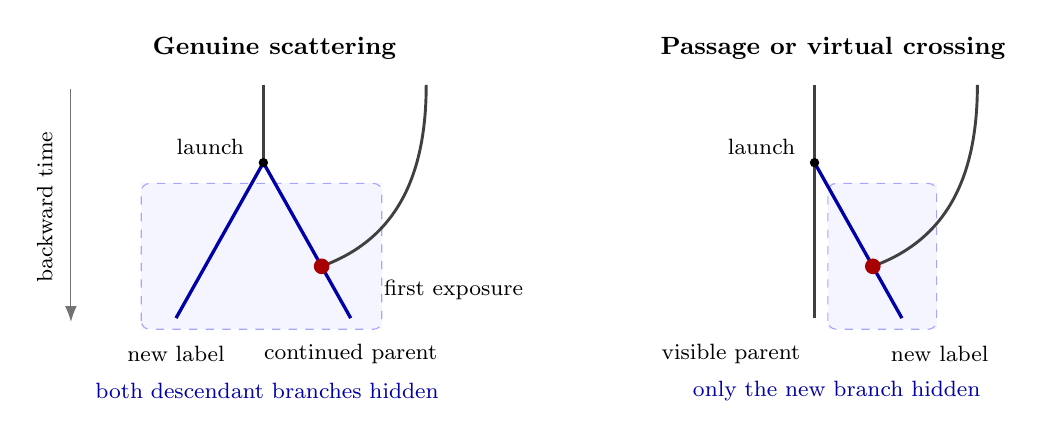
\begin{tikzpicture}[x=0.94cm,y=0.94cm,
 visible/.style={draw=black!75,line width=1.05pt},
 hidden/.style={draw=blue!65!black,line width=1.2pt},
 every node/.style={font=\small},
 exposure point/.style={circle,fill=red!65!black,inner sep=2pt}]
\draw[-{Latex[length=2mm]},black!55] (-2.6,3.1)--(-2.6,-.05);
\node[rotate=90,anchor=south,font=\footnotesize] at (-2.72,1.5)
 {backward time};
\begin{scope}
 \node[font=\small\bfseries] at (.15,3.65) {Genuine scattering};
 \fill[blue!4] (-1.65,-.15) rectangle (1.6,1.82);
 \draw[blue!35,dashed,rounded corners=3pt]
  (-1.65,-.15) rectangle (1.6,1.82);
 \draw[visible] (0,3.15)--(0,2.1);
 \draw[hidden] (0,2.1)--(-1.18,0);
 \draw[hidden] (0,2.1)--(1.18,0);
 \fill[black] (0,2.1) circle (1.7pt);
 \node[anchor=east,font=\footnotesize] at (-.13,2.32) {launch};
 \draw[visible] (2.2,3.15) .. controls (2.2,1.85) and (1.75,1.05)
  .. (.787,.7);
 \node[exposure point] at (.787,.7) {};
 \node[anchor=west,font=\footnotesize] at (1.5,.38) {first exposure};
 \node[align=center,font=\footnotesize] at (-1.18,-.48) {new label};
 \node[align=center,font=\footnotesize] at (1.18,-.48) {continued parent};
 \node[blue!65!black,font=\footnotesize] at (.05,-.98)
  {both descendant branches hidden};
\end{scope}
\begin{scope}[xshift=7cm]
 \node[font=\small\bfseries] at (.25,3.65) {Passage or virtual crossing};
 \fill[blue!4] (.18,-.15) rectangle (1.65,1.82);
 \draw[blue!35,dashed,rounded corners=3pt]
  (.18,-.15) rectangle (1.65,1.82);
 \draw[visible] (0,3.15)--(0,0);
 \draw[hidden] (0,2.1)--(1.18,0);
 \fill[black] (0,2.1) circle (1.7pt);
 \node[anchor=east,font=\footnotesize] at (-.13,2.32) {launch};
 \draw[visible] (2.2,3.15) .. controls (2.2,1.85) and (1.75,1.05)
  .. (.787,.7);
 \node[exposure point] at (.787,.7) {};
 \node[anchor=east,font=\footnotesize] at (-.06,-.48) {visible parent};
 \node[anchor=west,font=\footnotesize] at (.9,-.48) {new label};
 \node[blue!65!black,font=\footnotesize] at (.3,-.98)
  {only the new branch hidden};
\end{scope}
\end{tikzpicture}
\caption{The auxiliary exposure used to multiply contact savings.
Blue branches carry an unrevealed launch parameter. A genuine
scattering changes the continued parent's velocity, so both descendant
branches must be hidden. Passage leaves the parent unchanged.
Until first exposure, the black trajectories can be computed without
the hidden parameter. The construction is applied to exact signed
histories; no particles are deleted from the microscopic dynamics.
The drawing shows one selected tree. The full construction also omits
added groups whose positions have not yet been fixed relative to the
visible particles, including groups not selected for exposure;
Proposition~\ref{exp:exposure} gives the complete construction.}
\label{fig:exposure}
\end{figure}


Section~\ref{sec:preliminaries} establishes the flow, initial estimates,
scattering facts, and uniform smooth-input bounds.
Section~\ref{sec:cell-expansion} constructs the exact finite expansion.
Section~\ref{sec:centering} gives the centered identities and the
short-layer approximation to the kinetic solution.
Sections~\ref{sec:history-estimates} and~\ref{sec:exposure} prove the
finite-history measure estimates and the exposure bound.
Section~\ref{sec:closure} chooses the thresholds, removes every cutoff,
and proves Theorem~\ref{thm:main} and Corollary~\ref{cor:empirical}.

\clearpage
\section{Microscopic flow, scattering, and kinetic envelopes}
\label{sec:preliminaries}

The microscopic expansion uses globally defined finite-particle flows
and small initial centered correlations. We establish these facts,
identify the collision operator by two-body flux, and derive fixed
spatially summable Gaussian bounds for the assumed kinetic solution
and its spatial gradient. The scattering arguments require neither a
monotone potential nor a regular differential cross-section.

\subsection{Potential assumptions and finite-particle flow}

\begin{assumption}[Potential class]\label{pre:potential}
Write $\Phi(q)=\phi(|q|)$, with $\Phi(q)=0$ for $|q|\geq1$.
Assume either $\Phi\in C^2(\mathbb R^3;\mathbb R)$, or
$\Phi\in C^2(\mathbb R^3\setminus\{0\})$ with
$\Phi(q)\to+\infty$ as $q\to0$.
In the latter case set $\Phi(0)=+\infty$.
Assume thermodynamic stability: for some $B\geq0$,
\begin{equation}\label{eq:pre-stability}
 \sum_{\substack{i,j\in R\\i<j}}\Phi(q_i-q_j)\geq-B|R|
\end{equation}
for every finite configuration of distinct points.
The potential is fixed independently of $\varepsilon$.
\end{assumption}

These are the assumptions of Hypothesis $1'$ in
\cite[Section 8]{PSS14}. Set
\[
 \Phi_\varepsilon(x)=\Phi(x/\varepsilon),\qquad
 \mathscr H_R(Z_R)=\frac12\sum_{i\in R}|v_i|^2+
       \sum_{\substack{i,j\in R\\i<j}}\Phi_\varepsilon(x_i-x_j).
\]
The exact microscopic equations are
\begin{equation}\label{pre:dynamics}
 \dot x_i=v_i,\qquad
 \dot v_i=-\frac1\varepsilon\sum_{j\in R\setminus\{i\}}
             \nabla\Phi((x_i-x_j)/\varepsilon).
\end{equation}

\begin{proposition}[Global finite-particle flow]\label{pre:flow}
For each fixed $\varepsilon>0$ and finite label set $R$,
\eqref{pre:dynamics} has a unique global flow from every finite-energy
initial state in its domain. The flow preserves phase volume and
$\mathscr H_R$. In the singular case, every pair distance along a given
trajectory is bounded away from zero. In the nonsingular case coincident
positions are permitted.
\end{proposition}

\begin{proof}
Taking two particles in \eqref{eq:pre-stability} gives
$\phi(r)\geq-2B$ for $r>0$. In the nonsingular case, approximation by
distinct configurations extends stability to coincident positions.
The vector field is locally Lipschitz on its domain and hence has a
unique maximal local solution. Differentiation gives energy conservation
on its existence interval. For $n=|R|$,
\begin{equation}\label{eq:pre-speed}
 \frac12\sum_{i\in R}|v_i(t)|^2
       \leq\mathscr H_R(Z_R(0))+Bn.
\end{equation}
For $n\geq2$, bounding every pair except one below gives
\begin{equation}\label{eq:pre-pairupper}
 \Phi_\varepsilon(x_i(t)-x_j(t))
 \leq\mathscr H_R(Z_R(0))
             +2B\left(\binom n2-1\right).
\end{equation}
In the singular case this bounds every pair distance away from zero.
Equation \eqref{eq:pre-speed} prevents escape to spatial infinity in
finite time. Thus on each bounded time interval the solution remains in
a compact subset of the vector field's domain and extends beyond any
proposed finite endpoint, forward or backward. In the nonsingular case
one can also use the globally Lipschitz gradient of the compactly
supported $C^2$ potential directly. The cases $n=0,1$ are immediate.

The vector field has zero divergence in $(x_i,v_i)_{i\in R}$:
$\dot x_i$ is independent of $x_i$ and $\dot v_i$ is independent of
$v_i$. Its flow Jacobian therefore solves $\dot J=0$ with $J(0)=1$.
\end{proof}

\subsection{The ensemble and external isolation}

\begin{definition}[Exact initial ensemble]
Let $\mu=\varepsilon^{-2}$ and
\[
 {\cal D}_R^\varepsilon
 =\{Z_R:|x_i-x_j|>\varepsilon\text{ for all }i\ne j\in R\}.
\]
For the prescribed $C^1$ nonnegative probability density $f_0$, set
\begin{align}
 {\cal Z}_\varepsilon
 &=\sum_{n=0}^\infty\frac{\mu^n}{n!}
   \int f_0^{\otimes n}(Z_n)
             \mathbf1_{{\cal D}_{[n]}^\varepsilon}(Z_n)\,dZ_n,
       \label{eq:pre-partition}\\
 W_{0,n}(Z_n)
 &={\cal Z}_\varepsilon^{-1}\mu^n f_0^{\otimes n}(Z_n)
             \mathbf1_{{\cal D}_{[n]}^\varepsilon}(Z_n).
       \label{eq:pre-ensemble}
\end{align}
Here $[n]=\{1,\ldots,n\}$ and empty products equal one.
The probability law on ordered coordinates is
\begin{equation}\label{pre:model}
 \mathbb P(N=n,Z_n\in dZ_n)=\frac1{n!}W_{0,n}(Z_n)\,dZ_n.
\end{equation}
Thereafter the cloud evolves by \eqref{pre:dynamics}.
\end{definition}

Since $1\leq\mathcal Z_\varepsilon\leq e^\mu$, this is a probability law
with finite $N$ almost surely. Initial exclusion gives zero potential
energy and finite kinetic energy. Proposition~\ref{pre:flow} therefore
defines its exact evolution. Let $W_{t,n}$ be the transported density.

For $r=|R|$, the rescaled factorial density is
\begin{equation}\label{pre:factorial}
 F_R^\varepsilon(t,Z_R)=
 \mu^{-r}\sum_{n=0}^\infty\frac1{n!}
       \int W_{t,r+n}(Z_R,Z_{[n]}^{\rm ext})\,dZ_{[n]}^{\rm ext}.
\end{equation}
External labels are distinct from those in $R$.
Symmetry makes the formula independent of their temporary names.
It equals the density defined by the ordered distinct-label sum in the
statement: in a cloud of size $r+n$, there are $(r+n)!/n!$ such selections.

The externally isolated factorial density is
\begin{equation}\label{eq:pre-isolated}
 \widetilde F_R^\varepsilon(t,Z_R)=
 \mu^{-r}\sum_{n=0}^\infty\frac1{n!}
 \int W_{t,r+n}(Z_R,Z_{[n]}^{\rm ext})
 \prod_{\substack{i\in R\\j\in[n]^{\rm ext}}}
       \mathbf1_{\{|x_i-x_j|>\varepsilon\}}\,
             dZ_{[n]}^{\rm ext}.
\end{equation}
Set $F_\varnothing^\varepsilon=\widetilde F_\varnothing^\varepsilon=1$.
External isolation imposes no condition on distances within $R$.
In particular an interacting displayed component can be externally
isolated, and $0\leq\widetilde F_R^\varepsilon\leq F_R^\varepsilon$.
A polymer is a connected component of the instantaneous graph with
edges $|x_i-x_j|\leq\varepsilon$.
The condition in \eqref{eq:pre-isolated} says exactly that the displayed
labels form a union of entire polymers of the full cloud.

\begin{proposition}[Initial insertion and centering]\label{pre:initial}
Put $\rho_0(x)=\int f_0(x,v)\,dv$, and assume $\|\rho_0\|_\infty<\infty$.
At time zero,
\begin{equation}\label{eq:pre-insertion}
 \begin{split}
 \widetilde F_R^\varepsilon(0,Z_R)
 &=F_R^\varepsilon(0,Z_R)\\
 &=f_0^{\otimes R}(Z_R)\mathbf1_{{\cal D}_R^\varepsilon}(Z_R)
       \mathbb E\prod_{i\in R}\mathbf1_{\{N(B_i)=0\}},
 \qquad B_i=\overline B(x_i,\varepsilon).
 \end{split}
\end{equation}
The expectation is over an independent cloud with the original law,
and $N(B)$ counts its positions in $B$.
Consequently $0\leq F_R^\varepsilon(0)\leq f_0^{\otimes R}$.

For $Z_R\in{\cal D}_R^\varepsilon$, define
\begin{equation}\label{eq:pre-initialcenter}
 E_R^\varepsilon(0,Z_R)=
 \sum_{S\subset R}(-1)^{|R\setminus S|}
      f_0^{\otimes(R\setminus S)}(Z_{R\setminus S})
      \widetilde F_S^\varepsilon(0,Z_S).
\end{equation}
There are $c_0>0,C_0<\infty$, independent of $R,\varepsilon$, such that
for sufficiently small $\varepsilon$,
\begin{equation}\label{eq:pre-centersmall}
 |E_R^\varepsilon(0,Z_R)|
       \leq(C_0\varepsilon^{c_0})^{|R|}f_0^{\otimes R}(Z_R).
\end{equation}
One may take $c_0=1/125$.
For fixed $r$,
\begin{equation}\label{eq:pre-mass}
 0\leq1-\int F_R^\varepsilon(0,Z_R)\,dZ_R
       \leq Cr\varepsilon+Cr^2\varepsilon^3,
 \qquad \int F_R^\varepsilon(t)=\int F_R^\varepsilon(0).
\end{equation}
\end{proposition}

\begin{proof}
Insert $r$ particles into \eqref{pre:factorial} at time zero.
Their mutual exclusions give $\mathbf1_{{\cal D}_R^\varepsilon}$.
The remaining partition sum is $\mathcal Z_\varepsilon$ times the
probability that the original cloud misses $\bigcup_iB_i$.
This proves \eqref{eq:pre-insertion}. Initial exclusion already gives
external isolation.

On $\mathcal D_R^\varepsilon$ every subset is separated, so substitution
into \eqref{eq:pre-initialcenter} gives the exact identity
\begin{equation}\label{eq:pre-occupancy}
 E_R^\varepsilon(0,Z_R)
 =(-1)^{|R|}f_0^{\otimes R}(Z_R)
       \mathbb P\{N(B_i)\geq1\text{ for every }i\in R\}.
\end{equation}
Choose a maximal subcollection of centers with mutual distance greater
than $2\varepsilon$. Its balls $B_i$ are disjoint up to null boundaries.
A ball of radius $2\varepsilon$ contains at most $125$ original centers:
their disjoint balls of radius $\varepsilon/2$ fit inside a ball of
radius $5\varepsilon/2$. Hence the chosen subcollection has size
$m\geq |R|/125$. Disjointness ensures that occupants are distinct, and
the factorial upper bound gives
\begin{align*}
 \mathbb P\{N(B_i)\geq1\text{ for every chosen }i\}
 &\leq\mathbb E\prod_{\text{chosen }i}N(B_i)\\
 &=\mu^m\int_{\prod_i(B_i\times\mathbb R^3)}
                          F_m^\varepsilon(0)\,dZ_m\\
 &\leq\bigl(\mu\|\rho_0\|_\infty|B(0,\varepsilon)|\bigr)^m
 \leq(C\varepsilon)^m.
\end{align*}
For $C\varepsilon\leq1$ this proves \eqref{eq:pre-centersmall}.

The loss from mutual exclusion of $r$ independent inserted positions
is at most $Cr^2\varepsilon^3$, by a union bound and bounded $\rho_0$.
For each inserted position,
\[
 \mathbb P\{N(B_i)\geq1\}\leq\mathbb E N(B_i)
 =\mu\int_{B_i\times\mathbb R^3}F_1^\varepsilon(0,z)\,dz
 \leq C\varepsilon.
\]
A second union bound proves the first estimate in \eqref{eq:pre-mass}.
The integral of \eqref{pre:factorial} is
$\mu^{-r}\mathbb E(N)_r$, where
$(N)_r=N(N-1)\cdots(N-r+1)$.
It is finite by the initial factorial bound and conserved since $N$ is
conserved.
\end{proof}

\subsection{Scattering flux and the collision operator}

Use microscopic relative coordinates in this subsection.
For $g\ne0$ and $b\in g^\perp$, $|b|<1$, the incoming free trajectory
meets the interaction sphere at
\[
 n=b-\sqrt{1-|b|^2}\,\frac g{|g|},\qquad n\cdot g<0.
\]
Time translation identifies the asymptotic prescription
$q(\tau)-(b+\tau g)\to0$, $q'(\tau)\to g$ as $\tau\to-\infty$,
with $q(0)=n$, $q'(0)=g$ for $q''=-2\nabla\Phi(q)$.
Let $\tau_*(n,g)\in(0,\infty]$ be its first subsequent exit time from
the open unit ball.
Projection onto the impact disk has Jacobian
\begin{equation}\label{eq:pre-fluxdisk}
 |n\cdot g|\,d\sigma(n)=|g|\,d^2b.
\end{equation}

\begin{lemma}[Residence-time flux]\label{pre:duration}
For every $M<\infty$ there is $C_M<\infty$ such that
\begin{equation}\label{eq:pre-duration}
 \int_{\substack{|g|\leq M\\n\in S^2,\ n\cdot g<0}}
 \tau_*(n,g)|n\cdot g|\,d\sigma(n)\,dg\leq C_M.
\end{equation}
The incoming flux of $\{\tau_*>D,\ |g|\leq M\}$ is at most $C_M/D$.
In particular $\tau_*<\infty$ almost everywhere in incoming flux.
The entrance-to-exit scattering map preserves flux.
\end{lemma}

\begin{proof}
Relative energy is
\[
 \tfrac14|q'|^2+\phi(|q|)=\tfrac14|g|^2.
\]
Since $\phi\geq-2B$, we have $|q'|^2\leq M^2+8B$ throughout the
encounter. Consider
\[
 (n,g,s)\longmapsto(q(s),q'(s)),
 \quad n\cdot g<0,\quad |g|\leq M,\quad0<s<\tau_*(n,g).
\]
Its volume element is $|n\cdot g|\,d\sigma(n)\,dg\,ds$.
At $s=0$, append the velocity vector field to five tangent vectors of
the entrance section. Its normal component in position space is
$n\cdot g$. Phase-volume preservation propagates that determinant.

The map is injective. Two representations of an interior state lie on
the same orbit by uniqueness. A preceding outward crossing cannot be
followed by an inward crossing: outside the ball the path is a
straight line with increasing distance from the origin. If the orbit
repeated an interior state it would be periodic, so it could not have
a past entrance from outside. Hence there is at most one entrance and
elapsed time.

Apply change of variables on compact pieces of the entrance section
and bounded elapsed-time intervals, then exhaust the domain.
The image lies in $B(0,1)\times B(0,\sqrt{M^2+8B})$.
Its finite volume proves \eqref{eq:pre-duration}.
Markov's inequality gives the tail and excludes infinite duration
outside a null set. The same flow-box determinant on the transverse
exit section proves flux preservation. Tangential section data carry
zero flux.
\end{proof}

\begin{definition}[The scattering collision operator]
Write $c=(v+v_*)/2$, $g=v-v_*$, and, for almost every incoming datum,
let $g_{\rm out}$ be the velocity after exit. Set
\[
 v'=c+\tfrac12g_{\rm out},\qquad
 v_*'=c-\tfrac12g_{\rm out}.
\]
For $\psi\in C_c^\infty(\mathbb R^3)$, define $Q_\Phi$ at each $x$ by
\begin{equation}\label{pre:collision}
 \begin{split}
 \int Q_\Phi(f,f)(x,v)\psi(v)\,dv
 =\frac12\int_{\mathbb R^3\times\mathbb R^3}
 & f(x,v)f(x,v_*)|v-v_*|\\
 {}\times\int_{\substack{b\in(v-v_*)^\perp\\|b|<1}}
 &[\,\psi(v')+\psi(v_*')-\psi(v)-\psi(v_*)\,]\,
                         d^2b\,dv\,dv_* .
 \end{split}
\end{equation}
Here $d^2b$ is Euclidean area, and the $g=0$ contribution is zero.
Null exceptional scattering data are ignored.
\end{definition}

\begin{lemma}[Reversibility and normalization]\label{pre:operator}
The measure $d\Lambda=|v-v_*|\,dv\,dv_*\,d^2b$ is preserved by
exchanging incoming and outgoing velocity pairs with the corresponding
entrance parameter. The weak definition \eqref{pre:collision} equals
\begin{equation}\label{eq:pre-Qstrong}
 Q_\Phi(f,f)(x,v)=
 \int_{\mathbb R^3}|v-v_*|
 \int_{\substack{b\in(v-v_*)^\perp\\|b|<1}}
 [\,f(x,v')f(x,v_*')-f(x,v)f(x,v_*)\,]\,d^2b\,dv_* .
\end{equation}
These identities hold whenever the integrals are absolutely convergent,
in particular for Gaussian bounded functions. All scattering branches
are included, and the impact disk has area $\pi$.
\end{lemma}

\begin{proof}
Let $(n_+,g_{\rm out})$ be the exit state of the relative orbit with
entrance $(n,g)$. Since $\Phi$ is even, $-q(\tau_*-s)$ has entrance
$(-n_+,g_{\rm out})$ and exit $(-n,g)$.
Thus $(n,g)\mapsto(-n_+,g_{\rm out})$ is an involution of the incoming
section outside a null set. It preserves flux by
Lemma~\ref{pre:duration} and the reflection $n_+\mapsto-n_+$.
The center velocity is unchanged, and
$(v,v_*)\leftrightarrow(c,g)$ has absolute determinant one.
Equation \eqref{eq:pre-fluxdisk} proves invariance of $d\Lambda$.

Particle exchange also preserves $d\Lambda$, so the two test-function
terms in either pair of \eqref{pre:collision} give equal integrals.
This cancels the factor $1/2$. The scattering involution transfers
the remaining outgoing test to the incoming variable, giving
\eqref{eq:pre-Qstrong}.
Energy conservation gives
$|v'|^2+|v_*'|^2=|v|^2+|v_*|^2$.
The finite disk area and Gaussian integration justify absolute
convergence. No scattering-angle density or choice of one branch is
introduced.
\end{proof}

\subsection{Exceptional deflections and rotational parameters}

\begin{proposition}[Scattering nondegeneracy]\label{pre:scattering}
Outside a set of zero incoming flux, an encounter either is a straight
force-free passage or satisfies
\begin{equation}\label{eq:pre-increments}
 v'\ne v,\qquad v_*'\ne v .
\end{equation}
For $M<\infty$ and $\eta>0$, the non-free relative incoming data $(n,g)$
with $|g|\leq M$
can be restricted to a rotation-invariant compact set, losing at most
$\eta$ relative incoming flux, on which the duration is bounded and
$|g|$, $|v'-v|$, and $|v_*'-v|$ have positive lower bounds.
For fixed radial scattering parameters, each of these nonzero
increments has a uniform spherical directional marginal under common
rotation. The two increments need not be independent.
\end{proposition}

\begin{proof}
Put $G=|g|$, $\rho=|b|$, $J=G\rho$, and $E=G^2/4$.
The cases $G=0$, $J=0$, and $\rho=1$ are null in incoming flux.
For $J>0$, the effective radial potential is
\[
 W_J(r)=\phi(r)+\frac{J^2}{4r^2}.
\]
An incoming turning radius $y$ satisfies $E=W_J(y)$.
A nonsimple turning point also requires $W_J'(y)=0$.
At each fixed $J$, the critical values of the $C^2$ function $W_J$ on
$(0,1)$ are Lebesgue null, by the one-dimensional Sard theorem on a
countable compact exhaustion. The radial incoming flux is
\begin{equation}\label{eq:pre-Sardflux}
 G^3\rho\,dG\,d\rho=2J\,dE\,dJ.
\end{equation}
Fubini excludes nonsimple turning energies up to zero flux.
Lemma~\ref{pre:duration} has already excluded infinite duration.

At a simple incoming turning radius $y\in(0,1)$,
$W_J'(y)<0$ and $E>W_J(r)$ for all $r>y$.
Set $a=J^{-2}$ and
\[
 A_y(r)=y^{-2}-r^{-2},\qquad
 C_y(r)=4(\phi(y)-\phi(r)),\qquad
 H_{y,a}(r)=A_y(r)+aC_y(r).
\]
The half angular sweep is
\begin{equation}\label{eq:pre-halfangle}
 {\cal A}_y(a)=\int_y^\infty\frac{dr}{r^2\sqrt{H_{y,a}(r)}}.
\end{equation}
Indeed $\dot r^2=J^2H_{y,a}(r)$ and the angular speed is $J/r^2$.
For admissible $a$, one has $H_{y,a}(r)>0$ for $r>y$,
$\partial_rH_{y,a}(y)>0$, and
$\lim_{r\to\infty}H_{y,a}(r)>0$.
The ratios $C_y/A_y$ and $H_{y,a}/A_y$ extend continuously to
$[y,\infty]$. At $y$ use the ratios of first derivatives; at infinity
use finite range. The second ratio is strictly positive on this compact
interval, so it has a positive minimum, while $C_y/H_{y,a}$ is bounded.
These properties also show that the admissible set of $a$ is open.

For $a'$ near $a$, the binomial expansion in
\[
 H_{y,a'}^{-1/2}
 =H_{y,a}^{-1/2}
       \left(1+(a'-a)\frac{C_y}{H_{y,a}}\right)^{-1/2}
\]
converges uniformly after multiplication by the integrable majorant
$r^{-2}H_{y,a}^{-1/2}$. Thus $\mathcal A_y$ is real analytic in the
parameter $a$, although $\phi$ is only $C^2$.
Twice differentiating gives
\begin{equation}\label{eq:pre-convex}
 {\cal A}_y''(a)=\frac34
       \int_y^\infty\frac{C_y(r)^2\,dr}{r^2H_{y,a}(r)^{5/2}}.
\end{equation}
Near $y$ the integrand is $O((r-y)^{-1/2})$, since $C_y(r)=O(r-y)$
and $H_{y,a}$ has a simple root. It is also integrable at infinity.
It is strictly positive unless $\phi(r)=\phi(y)$ for every $r\geq y$.
Finite range makes this constant zero; the encountered orbit is then
a straight force-free passage.

For a non-free encounter $\mathcal A_y$ is strictly convex.
The deflection angle is $\pi-2\mathcal A_y$ modulo $2\pi$.
Therefore $g_{\rm out}=g$ or $g_{\rm out}=-g$ requires
$\mathcal A_y\in(\pi/2)\mathbb Z$.
Each such level has at most two preimages on an admissible interval.
There are countably many levels and countably many open intervals.
On a simple turning branch, $(y,J)\mapsto(E,J)$, $E=W_J(y)$,
is a local $C^1$ diffeomorphism.
A countable cover by these charts, Fubini in $(y,a)$, and
\eqref{eq:pre-Sardflux} prove flux nullness.
These exceptional equalities are exactly the two failures of
\eqref{eq:pre-increments}.

For the compact-set assertion, exhaust the simple-scattering non-free
radial parameter domain by compact subsets avoiding $G=0$, $J=0$,
$\rho=1$, and the zero-increment levels.
This covers all non-free data outside a null set.
On each such compact subset, continuous dependence for the $C^1$
ODE flow and transversality of the finite exit give a continuous
exit time and scattering map. Thus durations are bounded and all the
listed nonzero quantities have positive minima.
The relative flux measure on $G\leq M$ is finite, so an exhaustion
member loses at most $\eta$ flux. Lifting with all rotations makes
the set rotation-invariant.

Finally, write $(g,b)=(GRe_1,\rho Re_2)$, $R\in SO(3)$.
At fixed $(G,\rho)$ the orientation factor in incoming flux is a
constant multiple of Haar measure on $SO(3)$.
Central-force rotation equivariance maps each nonzero increment to
$R$ times a fixed vector. Its direction has uniform measure on $S^2$.
This is a marginal statement and leaves the joint pair correlated.
\end{proof}

\subsection{A fixed spatial Gaussian envelope on the kinetic interval}

Use the norm $\|\cdot\|_{\mathrm{Bol},\alpha}$ defined in
\eqref{intro:norm}, and put
\[
 \|h\|_{\infty,\alpha}
       =\sup_{x,v}e^{\alpha|v|^2}|h(x,v)|.
\]
For vector-valued functions use Euclidean norm.
The following proof adapts the weighted transport estimate in
\cite[Proposition A.1]{DHM25}. Only finite impact area and kinetic
energy conservation are needed, so the argument applies to $Q_\Phi$.

\begin{proposition}[Known-solution envelopes]\label{pre:envelopes}
Suppose $f$ is the classical nonnegative solution in the statement, and
\[
 A=\sup_{0\leq t\leq T}\|f(t)\|_{\infty,2\beta}<\infty,\qquad
 B_0=\|f_0\|_{\mathrm{Bol},2\beta}
               +\|\nabla_xf_0\|_{\mathrm{Bol},2\beta}<\infty.
\]
Then
\begin{equation}\label{eq:pre-envelope}
 \sup_{0\leq t\leq T}
 \left(\|f(t)\|_{\mathrm{Bol},\beta}
       +\|\nabla_xf(t)\|_{\mathrm{Bol},\beta}\right)
       \leq C(A,B_0,\beta,T)<\infty.
\end{equation}
Fix, once and for all,
\begin{equation}\label{eq:pre-beta0}
 \beta_0=\beta/2.
\end{equation}
Thus all independent inputs $f(t)$ and their spatial Lipschitz
envelopes have a common bound with the fixed margin
$\beta-\beta_0$. Constants in \eqref{eq:pre-envelope} are independent
of the subsequent time-layer subdivision.
\end{proposition}

\begin{proof}
Set
\[
 \gamma(t)=\frac{3\beta}{2}-\frac{\beta t}{2T},\qquad
 c=\frac{\beta}{2T},\qquad M(v)=e^{-2\beta|v|^2},
\]
and $(S(r)h)(x,v)=h(x-rv,v)$.
Notice $\beta\leq\gamma(t)\leq3\beta/2$.
Define a positive linear operator for $h\geq0$ by
\begin{equation}\label{eq:pre-positiveB}
 \begin{split}
 ({\cal B}h)(x,v)=\int_{\mathbb R^3}|v-v_*|\int_{|b|<1}
 \bigl[&M(v_*')h(x,v')+M(v')h(x,v_*')\\
       &+M(v_*)h(x,v)+M(v)h(x,v_*)\bigr]\,d^2b\,dv_* .
 \end{split}
\end{equation}
The disk is in $(v-v_*)^\perp$.

We first prove that for $0\leq s<t\leq T$, $r=t-s$,
\begin{align}
 \|S(r){\cal B}h\|_{\mathrm{Bol},\gamma(t)}
       &\leq Cr^{-1/2}\|h\|_{\mathrm{Bol},\gamma(s)},
                    \label{eq:pre-VolterraBol}\\
 \|S(r){\cal B}h\|_{\infty,\gamma(t)}
       &\leq Cr^{-1/2}\|h\|_{\infty,\gamma(s)}.
                    \label{eq:pre-Volterrainfty}
\end{align}
Let $H_s(y)=\sup_u e^{\gamma(s)|u|^2}h(y,u)$.
For each product in \eqref{eq:pre-positiveB}, energy conservation,
or its identity version for a loss product, gives
\[
 M(u_*)h(y,u)
       \leq H_s(y)e^{-\gamma(s)(|v|^2+|v_*|^2)}.
\]
After multiplication by $e^{\gamma(t)|v|^2}$ this is at most
\[
 H_s(y)e^{-\beta|v_*|^2}
                    e^{-cr(|v|^2+|v_*|^2)}.
\]
Since
\[
 |v-v_*|e^{-cr(|v|^2+|v_*|^2)/2}\leq C_c r^{-1/2},
\]
the disk area $\pi$ and the Gaussian integral in $v_*$ imply
\begin{equation}\label{eq:pre-spatialmajorant}
 e^{\gamma(t)|v|^2}(S(r){\cal B}h)(x,v)
       \leq Cr^{-1/2}e^{-cr|v|^2/2}H_s(x-rv).
\end{equation}
This proves \eqref{eq:pre-Volterrainfty}.

For the summed spatial estimate put
$a_k=\sup_{|y-k|\leq1}H_s(y)$.
If $m\leq r|v|<m+1$ and $|x-k|\leq1$, then
$|x-rv-k|\leq m+2$, whence
\[
 H_s(x-rv)\leq
       \sum_{\substack{\ell\in\mathbb Z^3\\|\ell-k|\leq m+3}}a_\ell.
\]
Indeed lattice-centered unit balls cover $\mathbb R^3$.
For $r\leq T$, the damping factor on that shell is at most
$e^{-cm^2/(2T)}$.
Bound the supremum over $v$ by summation over $m\geq0$ and then sum
over $k$. Each $a_\ell$ occurs at most $C(m+4)^3$ times.
Convergence of
$\sum_{m\geq0}e^{-cm^2/(2T)}(m+4)^3$ proves
\eqref{eq:pre-VolterraBol}.
The same shell argument, now using
\[
 e^{\gamma(t)|v|^2}|S(t)h_0(x,v)|
 \leq e^{-ct|v|^2}
       \sup_u e^{\gamma(0)|u|^2}|h_0(x-tv,u)|,
\]
gives
\begin{equation}\label{eq:pre-freebound}
 \sup_{0\leq t\leq T}\|S(t)h_0\|_{\mathrm{Bol},\gamma(t)}
       \leq C\|h_0\|_{\mathrm{Bol},\gamma(0)}.
\end{equation}
At $t=0$ this is immediate.

Define
\[
 ({\cal V}h)(t)=A\int_0^t S(t-s){\cal B}h(s)\,ds.
\]
The characteristic equation, $f\geq0$, and $f\leq AM$ imply
\begin{equation}\label{eq:pre-linearcomparison}
 0\leq f(t)\leq S(t)f_0+({\cal V}f)(t).
\end{equation}
Its $n$-fold iteration is the finite inequality
\[
 f\leq\sum_{j=0}^{n-1}{\cal V}^j(S(\cdot)f_0)+{\cal V}^n f.
\]
No finiteness of the unknown summed spatial norm has been assumed.
Using \eqref{eq:pre-Volterrainfty} and
$\|f(t)\|_{\infty,\gamma(t)}\leq A$ yields
\begin{equation}\label{eq:pre-remaindergamma}
 \|({\cal V}^n f)(t)\|_{\infty,\gamma(t)}
       \leq A\frac{(CA\Gamma(1/2))^nt^{n/2}}
                           {\Gamma(1+n/2)}.
\end{equation}
This tends to zero uniformly for $t\leq T$.
The time-convolution formula follows inductively from
\[
 \int_0^t(t-s)^{-1/2}s^{n/2}\,ds
 =t^{(n+1)/2}
       \frac{\Gamma(1/2)\Gamma(1+n/2)}
            {\Gamma(1+(n+1)/2)}.
\]
Equations \eqref{eq:pre-VolterraBol} and
\eqref{eq:pre-freebound} bound the summed spatial norm of the
$j$th series term by
\[
 C B_0\frac{(CA\Gamma(1/2))^jT^{j/2}}{\Gamma(1+j/2)}.
\]
The sum is finite. Letting $n\to\infty$ in the pointwise comparison
and then taking the summed spatial norm proves the required bound
for $f$ at exponent $\gamma(t)$.

To handle the derivative without assuming its envelope, fix a
coordinate unit vector $e$ and $0<|\delta|\leq1$, and put
\[
 d_\delta(t,x,v)
       =\frac{f(t,x+\delta e,v)-f(t,x,v)}{\delta}.
\]
Use $a'b'-ab=(a'-a)b'+a(b'-b)$ for both gain and loss products in
\eqref{eq:pre-Qstrong}. Each undifferenced factor is a spatial
translate of $f$, bounded by $AM$, so
\[
 |d_\delta(t)|
       \leq S(t)|d_\delta(0)|+{\cal V}|d_\delta|(t).
\]
For fixed $\delta$,
$\|d_\delta(t)\|_{\infty,\gamma(t)}\leq2A/|\delta|$.
The remainder argument \eqref{eq:pre-remaindergamma} therefore
applies and vanishes as $n\to\infty$, before taking $\delta\to0$.
The fundamental theorem of calculus gives
\[
 |d_\delta(0,x,v)|
       \leq\int_0^1|\partial_e f_0(x+\theta\delta e,v)|\,d\theta.
\]
Translations of length at most one change the summed spatial
supremum norm by at most an absolute factor, since each translated
unit ball is covered by a fixed number of lattice-centered unit
balls and each covering ball occurs a bounded number of times.
Hence
$\|d_\delta(0)\|_{\mathrm{Bol},\gamma(0)}\leq CB_0$,
uniformly in $\delta$.
The same series estimate bounds
$\|d_\delta(t)\|_{\mathrm{Bol},\gamma(t)}$ uniformly in $t,\delta$.
Pointwise convergence to $\partial_e f$, followed by Fatou's
inequality for the sum of local suprema, gives the derivative
bound. Sum over the three coordinate directions and use
$\gamma(t)\geq\beta$ to obtain \eqref{eq:pre-envelope}.
\end{proof}

\begin{remark}\label{pre:no-manybody-conclusion}
Lemma~\ref{pre:duration} concerns isolated two-body encounters, not
dynamically formed many-particle bound components.
Proposition~\ref{pre:scattering} supplies rotational marginals, not
independence from a trajectory that already depends on the same
parameters. The history estimates must establish the required
many-particle and conditional parameter statements separately.
\end{remark}

\section{An exact finite expansion on one cell}
\label{sec:cell}
\label{sec:cell-expansion}

The identities in this section concern a finite cloud.  In particular, they
do not assume that large components, recollisions, or long encounters are
unlikely.  Their signed auxiliary trajectories are distinguished throughout
from the trajectory of the full microscopic cloud. The use of autonomous
physical trajectory components and signed geometric overlap constraints
has its antecedent in~\cite{BGSSCluster2022}. For smooth potentials,
the identities below retain entire interacting components and their
potential energy.

\subsection{Contact components and kernels}

Fix a cell $I=[a,b]$, put $\delta=b-a$, and let $S$ be a finite label set.
For $A\subset S$ write
\[
 X_i^A(u;Z_A),\quad V_i^A(u;Z_A),\qquad i\in A,\quad 0\leq u\leq\delta,
\]
for the isolated Hamiltonian flow of precisely the labels in $A$, started
from $Z_A$ at $a$.  The empty flow has its evident meaning.  Statements about
these flows are made outside their null sets of undefined initial data.
The flow and its measurability are supplied by Proposition~\ref{pre:flow}.

Let $\pi_0(S)=\pi_0(Z_S)$ be the partition into connected components of
the graph with edges $|x_i-x_j|\leq\varepsilon$.  A subset is
\emph{initially admissible} if it is a union of blocks of $\pi_0(S)$.
Let $\Pi_I(A)$ be the connected-component partition of the graph on $A$
with an edge $ij$ whenever
\[
 \min_{0\leq u\leq\delta}|X_i^A(u)-X_j^A(u)|\leq\varepsilon.
\]
Thus a contact includes a force-free passage or a tangency.  Set
\[
 c_I(A)=\mathbf 1_{\{\Pi_I(A)=\{A\}\}}\quad(A\ne\varnothing),
 \qquad
 c_I^R(A)=\mathbf 1_{\{\text{every block of }\Pi_I(A)\text{ meets }R\}},
 \quad R\subset A.
\]
The latter indicator is one for $A=R=\varnothing$.  It is zero for
nonempty $A$ and empty $R$.

If $A$ and $B$ are disjoint, their two trajectories in the following
definition are computed \emph{separately}:
\[
 \tau_I(A,B)=\mathbf 1_{\{\exists u\in[0,\delta],\ i\in A,\ j\in B:
             |X_i^A(u)-X_j^B(u)|\leq\varepsilon\}},
 \qquad \alpha_I(A,B)=1-\tau_I(A,B).
\]
For a collection $\mathcal B$ of disjoint force groups, use
\[
 \tau_I(\mathcal B,C)=1-\prod_{B\in\mathcal B}\alpha_I(B,C).
\]
The union of groups in $\mathcal B$ is not assigned a new interacting
flow in this notation.  Its paths remain the indicated separate paths.
For a prescribed collection of paths $\mathcal X$ and a remaining cloud
$V$, define
\begin{equation}
 \Xi_I(\mathcal X;V)
 =\prod_{C\in\Pi_I(V)}\bigl(1-\tau_I(\mathcal X,C)\bigr).
 \label{eq:cell-Xi}
\end{equation}
The components on the right follow their isolated flows, which coincide
with their restrictions of the $V$-flow.  Empty products are one.

For $R\subset A$ the endpoint isolation indicator is
\[
 e_I^R(A)=\prod_{i\in R}\prod_{j\in A\setminus R}
       \mathbf 1_{\{|X_i^A(\delta)-X_j^A(\delta)|>\varepsilon\}}.
\]
It imposes no separation between two labels of $R$.  Introduce the
positive measure kernel
\begin{equation}
 \mathsf H^I_{R,A}(Z_A;\dd Y_R)
   =e_I^R(A)\,
     \delta_{(X_i^A(\delta),V_i^A(\delta))_{i\in R}}(\dd Y_R).
 \label{eq:cell-H}
\end{equation}
The Dirac measure notation avoids introducing a density for a
lower-dimensional transport kernel.

The only flow fact needed for the algebra is the following equivalence.
If separate groups avoid one another throughout $I$, their separate
flows are the restrictions of the flow of their union.  Conversely,
different blocks of $\Pi_I(S)$ avoid one another, and their restrictions
are isolated flows.  Indeed cross forces vanish in the first assertion,
so uniqueness proves it; the second follows from the definition of the
contact graph and the same uniqueness argument.

\begin{definition}[A cell diagram]
\label{def:cell-diagram}
For $R\subset S$, with $R\ne\varnothing$, a cell diagram on $(R,S)$ is
\[
 \gamma=(A;\Gamma_1,\ldots,\Gamma_\ell).
\]
Here $R\subset A\subset S$; the nonempty sets in all the $\Gamma_g$
together partition $S\setminus A$; and each $\Gamma_g$ is a nonempty
unordered collection of these sets.  Put $\Gamma_0=\{A\}$.
Different members of the diagram are different force groups.  Let
$\iota_0(\gamma)$ be the indicator that every force group in the diagram
is a union of blocks of $\pi_0(S)$.  Equivalently, all pairs in different
force groups have distance greater than $\varepsilon$ at $a$.
Define
\begin{align}
 w_I(\gamma;Z_S)
  ={}&\iota_0(\gamma)c_I^R(A)
       \prod_{g=1}^{\ell}
       \left[
        \prod_{B\in\Gamma_g}c_I(B)\tau_I(\Gamma_{g-1},B)
        \prod_{\{B,C\}\subset\Gamma_g}\alpha_I(B,C)
       \right],                                      \label{eq:cell-weight}\\
 \sigma(\gamma)={}&(-1)^{\sum_{g=1}^{\ell}|\Gamma_g|}.
                                                        \label{eq:cell-sign}
\end{align}
Only the root group $A$ uses a joint flow containing roots.  In
particular, a contact between different generations is a condition on
separate trajectories, not a force exerted between their groups.
The empty list of generations is allowed when $S=A$.
\end{definition}

Define the signed kernel
\begin{equation}
 \mathsf K^I_{R,S}(Z_S;\dd Y_R)
  =\sum_{\gamma\text{ on }(R,S)}
       \sigma(\gamma)w_I(\gamma;Z_S)
       \mathsf H^I_{R,A}(Z_A;\dd Y_R).
 \label{eq:cell-K}
\end{equation}
The sum is finite.  Set $\mathsf K^I_{\varnothing,\varnothing}=1$ and
$\mathsf K^I_{\varnothing,S}=0$ for $S\ne\varnothing$.
For a function or density $g$ on the input coordinates define
$\mathcal T^I_{R,S}g$ as a signed measure by
\begin{equation}
 \langle\psi,\mathcal T^I_{R,S}g\rangle
 =\int g(Z_S)\int\psi(Y_R)
                   \mathsf K^I_{R,S}(Z_S;\dd Y_R)\,\dd Z_S.
 \label{eq:cell-T}
\end{equation}

\begin{remark}[One additional label]
\label{rem:cell-single}
If an extra label $e$ is initially separate from all roots, its two
diagram terms are
\[
 c_I^R(R\cup\{e\})\mathsf H^I_{R,R\cup\{e\}}
 \; -\;
 \tau_I(R,\{e\})\mathsf H^I_{R,R}.
\]
The first follows the full force group and the second follows the
root group and a free extra particle separately.  If $e$ belongs to
an initial root polymer, it is mandatory and only the full-group term
is present.  No extra family-selection multiplicity is introduced
by this identity.
\end{remark}

\subsection{Boolean inversion and the generation identity}

\begin{proposition}[Exact cell expansion]
\label{cell:expansion}
Let $R\subset S$ and let $A_0$ be the union of the blocks of
$\pi_0(S)$ meeting $R$.  For $R\ne\varnothing$, let $\mathcal P$ be
the collection of the other blocks of $\pi_0(S)$.  Then
\begin{equation}
 \mathsf H^I_{R,S}
 =\sum_{\mathcal U\subset\mathcal P}
      \mathsf K^I_{R,A_0\cup\bigcup\mathcal U},
 \label{eq:cell-subset-sum}
\end{equation}
and, as an equality of signed measures,
\begin{equation}
 \mathsf K^I_{R,A_0\cup\bigcup\mathcal U}
  =\sum_{\mathcal V\subset\mathcal U}
       (-1)^{|\mathcal U|-|\mathcal V|}
       \mathsf H^I_{R,A_0\cup\bigcup\mathcal V}.
 \label{eq:cell-boolean}
\end{equation}
Every coefficient is evaluated on its displayed input coordinates.
If $m=|S\setminus R|$, the number of diagrams in
\eqref{eq:cell-K} is at most $(C(1+m))^{Cm}$, with a universal $C$.
There is no partition of the roots in this count.
\end{proposition}

\begin{proof}
First decompose the full flow according to its unique union of contact
components meeting $R$.  The flow observation preceding
Definition~\ref{def:cell-diagram} gives
\begin{equation}
 \mathsf H^I_{R,S}
 =\sum_{\substack{R\subset A\subset S\\
                   A\text{ union of blocks of }\pi_0(S)}}
       c_I^R(A)\mathsf H^I_{R,A}\Xi_I(\{A\};S\setminus A).
 \label{eq:cell-root-decomposition}
\end{equation}
Precisely one term has its two component indicators nonzero: the actual
union of rooted contact components.  Endpoint isolation of $R$ against
the rest of $S$ can then be checked inside $A$, because $A$ and its
complement avoid throughout the cell.

Here is the finite identity that expands the last factor.  Fix
$\mathcal X$, and consider a collection $\mathcal B$ of disjoint
nonempty subsets of $V$, each a union of the fixed initial polymers.
Put $U_{\mathcal B}=\bigcup\mathcal B$ and
\[
 d_I(\mathcal B)
   =\prod_{B\in\mathcal B}c_I(B)
      \prod_{\{B,C\}\subset\mathcal B}\alpha_I(B,C).
\]
Then
\begin{equation}
 \Xi_I(\mathcal X;V)
 =\sum_{\mathcal B}
       (-1)^{|\mathcal B|}d_I(\mathcal B)
       \prod_{B\in\mathcal B}\tau_I(\mathcal X,B)
       \Xi_I(\mathcal B;V\setminus U_{\mathcal B}).
 \label{eq:cell-generation-recursion}
\end{equation}
The term with $\mathcal B=\varnothing$ equals one.  To prove
\eqref{eq:cell-generation-recursion}, expand the product
\eqref{eq:cell-Xi} over subsets of its actual components.  A given
collection $\mathcal B$ consists of components of $V$ exactly when
its members are connected, mutually avoid, and avoid the remaining
$V\setminus U_{\mathcal B}$ flow.  These conditions are respectively
$\prod c_I(B)$, the pair product in $d_I$, and the last $\Xi_I$ in
\eqref{eq:cell-generation-recursion}.  On their support the required
flows agree.  This proves the formula, including all signs.

Apply \eqref{eq:cell-generation-recursion} repeatedly to
\eqref{eq:cell-root-decomposition}.  Every nonempty selection strictly
decreases the number of remaining labels, so the process terminates.
At termination its coefficient is exactly
\eqref{eq:cell-weight}--\eqref{eq:cell-sign}; the unselected labels
have no remaining restriction.  Grouping by the union of selected
initial polymers proves \eqref{eq:cell-subset-sum}.  The initial
partition of such a union is the restriction of $\pi_0(S)$, so its
coefficient is exactly the kernel defined in \eqref{eq:cell-K}, not a
kernel depending on unselected coordinates.  Finite Boolean inversion
proves \eqref{eq:cell-boolean}.

There are at most $2^m$ choices of $A\setminus R$, at most $m^m$
partitions of the remaining labels, and at most $m^m$ assignments of
their blocks to successive nonempty generations.  This proves the
count, with the cases $m=0,1$ understood separately.
\end{proof}

\subsection{Expectations and normalization}

For any finite random cloud let its scaled factorial measure with
external isolation be denoted by $\widetilde F_R$.  Its weak definition
is the usual factorial sum with the additional indicator that every
label outside the displayed set has distance greater than
$\varepsilon$ from it.  This definition permits internal contacts.
For the actual evolved initial ensemble, all exponential moments of
the total particle number are finite.  Indeed its initial probability
of $N=n$ is bounded by $\mu^n/n!$, and $N$ is conserved.

\begin{corollary}[Factorial normalization]
\label{cor:cell-factorial}
For the actual microscopic cloud and $r=|R|$, the cell identity is
written after relabelling the ordered roots as $R=\{1,\ldots,r\}$:
\begin{equation}
 \widetilde F_R(b)
  =\sum_{m\geq0}\frac{\mu^m}{m!}
       \mathcal T^I_{R,R\sqcup\{r+1,\ldots,r+m\}}
       \widetilde F_{r+m}(a).
 \label{eq:cell-factorial}
\end{equation}
The right side is interpreted with each finite Boolean coefficient
grouped before summing over $m$.  Equivalently, one may first restrict
the ensemble to $N\leq M$, apply the finite identity, and then let
$M\to\infty$.  No assertion of absolute summability of the
\emph{ungrouped} generation series is made here.
\end{corollary}

\begin{proof}
Apply \eqref{eq:cell-subset-sum} to each ordered tuple of roots in a
realization of the cloud at $a$.  A selected union of its initial
polymers is exactly an externally isolated displayed subset at $a$.
Consequently the expectation of each selected union uses
$\widetilde F_{r+m}(a)$.  Its $m$ extra labels were unordered, whereas
the factorial sum orders them, giving the divisor $m!$.  The scaling
of the original $r$ roots is $\mu^{-r}$, and that of the new factorial
measure is $\mu^{-(r+m)}$, giving $\mu^m$.

For a bounded test $\psi$, Boolean inversion bounds a coefficient
in total variation by $2^{|\mathcal U|}\|\psi\|_\infty$.  Summing this
over all selected polymer subsets in a fixed cloud costs at most
$3^N\|\psi\|_\infty$, and the root tuple count costs at most $N^r$.
The integrable bound $\mu^{-r}N^r3^N\|\psi\|_\infty$ justifies the
stated grouped limit.  Expanding every large-order coefficient into
all its diagrams before taking absolute values would give a different,
unproved convergence assertion and is unnecessary.
\end{proof}

\subsection{Factorization on all displayed trajectories}

\begin{proposition}[Diagramwise factorization]
\label{cell:factorization}
Split the labels into $S=S_1\sqcup S_2$ and the roots into
$R=R_1\sqcup R_2$, where $R_i\subset S_i$.  Let $\gamma_i$ be a
diagram on $(R_i,S_i)$.  Define $\eta_I(\gamma_1,\gamma_2)$ to be the
indicator that every displayed particle trajectory of $\gamma_1$
has distance greater than $\varepsilon$ throughout $I$ from every
displayed trajectory of $\gamma_2$.  This includes detached groups
and includes the initial and terminal times.
For a single global diagram $\gamma$, define
$\eta_I(\gamma;S_1,S_2)$ by the same condition between its labelled
paths in $S_1$ and $S_2$, using their prescribed force-group flows.

On this indicator, merge the two root groups, and take the union of
the two batches at each generation, padding a finished list by empty
batches.  This gives a diagram on $(R,S)$.  Conversely, every nonzero
diagram term satisfying $\eta_I(\gamma;S_1,S_2)=1$ splits uniquely in
this manner.  Its detached groups necessarily belong to one $S_i$,
and its root flow splits over its two intersections with $S_i$.
Under this bijection the signed transport measures, with this
indicator imposed, agree with the tensor product of the two
diagram transport measures:
\begin{equation}
 \sigma(\gamma)w_I(\gamma)\mathsf H^I_{R,A}\,\eta_I
  =\eta_I\bigl[
       \sigma(\gamma_1)w_I(\gamma_1)\mathsf H^I_{R_1,A_1}
       \otimes
       \sigma(\gamma_2)w_I(\gamma_2)\mathsf H^I_{R_2,A_2}
             \bigr].
 \label{eq:cell-factorization}
\end{equation}
Summation over the bijection preserves this equality.  Factorial
weights split as
\begin{equation}
 \binom{m_1+m_2}{m_1}
       \frac{\mu^{m_1+m_2}}{(m_1+m_2)!}
   =\frac{\mu^{m_1}}{m_1!}\frac{\mu^{m_2}}{m_2!}.
 \label{eq:cell-factorial-split}
\end{equation}
\end{proposition}

\begin{proof}
Cross avoidance makes the joint root flow equal to the two separate
root flows.  Its rooted-component and endpoint-isolation indicators
therefore split.  Initial-polymer admissibility also splits, since
all cross initial distances are greater than $\varepsilon$.
Within a merged generation, all additional cross avoidance factors
are one.  A detached component in $S_i$ can touch the preceding
generation only through that generation's $S_i$ part.  Hence its
touch indicator is exactly its original touch indicator.  The
number of detached groups is additive, so the signs multiply.
The output Dirac measures split with the root flow.  These facts
give \eqref{eq:cell-factorization}.

For the inverse map, a connected detached group cannot contain labels
from both families: a connected graph across that partition would
have a cross contact, contrary to $\eta_I=1$.  The same avoidance
splits the root group's flow by uniqueness.  A nonempty generation
in one family must have
a predecessor in that same family unless it is the first generation:
otherwise its required touch indicator vanishes.  There can therefore
be no gap followed by a later nonempty generation in one family.
Removing its terminal empty batches produces its unique local
generation list.  This proves the asserted bijection.  Formula
\eqref{eq:cell-factorial-split} is the ordinary ordered-label count.
\end{proof}

The avoidance condition in Proposition~\ref{cell:factorization} is
\emph{diagramwise}.  It is not a single condition on the flow of $S$.
For example, a third particle can deflect a prospective collision
partner away from a root in the full flow while a smaller subflow
still changes that root.  Such configurations are included in the
subset coefficient and cannot be removed using full-flow separation.
For more than two factors the proposition applies successively; its
indicator must include all displayed paths from all factors.  This
is the precise factorization used by the centered identities below.

\subsection{A deterministic stopped identity}

We give a stopped version before any probabilistic tail estimate.
Its stopping parameter $k$ counts all selected labels, including
the roots.  The threshold is allowed to include labels already
selected in later cells: in that case subtract that fixed offset
from the remaining threshold in the construction below.

Order components by the lexicographically least initial position in
each component; denote this position by $\kappa(C)\in\mathbb R^3$.
Different actual contact components have different such positions,
since particles with the same initial position belong to the same
initial polymer.  This is a measurable, label-equivariant deterministic
order.  The following elementary weighted product
identity is useful.  For $I_1,\ldots,I_n\in\{0,1\}$, positive integer
weights $w_1,\ldots,w_n$, and an integer $d>0$, let
$w(J)=\sum_{j\in J}w_j$.  Then
\begin{align}
 \prod_{j=1}^n(1-I_j)
 ={}&\sum_{\substack{J\subset\{1,\ldots,n\}\\w(J)<d}}
             (-1)^{|J|}\prod_{j\in J}I_j \nonumber\\
   &+\sum_{\substack{\varnothing\ne J\subset\{1,\ldots,n\}\\
                w(J\setminus\{\max J\})<d\leq w(J)}}
       (-1)^{|J|}\prod_{j\in J}I_j
                \prod_{j>\max J}(1-I_j).
 \label{eq:cell-stopped-product}
\end{align}
To verify it, expand the factors in their prescribed order, stopping
a branch at its first selected factor whose accumulated weight is
at least $d$.  Branches that finish without stopping are the first
sum, and stopped branches are the second.  The factors remaining
on a stopped branch lie in $[0,1]$.

Apply \eqref{eq:cell-stopped-product} to
$\Xi_I(\mathcal X;V)$, with the actual components of $V$ as its
ordered indices, $I_j=\tau_I(\mathcal X,C_j)$ and $w_j=|C_j|$.
For a selected collection $\mathcal B$, denote its last component
in this order by $B_*$ and set $V'=V\setminus U_{\mathcal B}$.
After extracting the selected components, the extra factor on
a stopped branch is
\begin{equation}
 \vartheta_I(\mathcal X,\mathcal B;V')
   =\Xi_I(\mathcal B;V')
      \prod_{\substack{C\in\Pi_I(V')\\
                   \kappa(C)>_{\mathrm{lex}}\kappa(B_*)}}
                  \bigl(1-\tau_I(\mathcal X,C)\bigr).
 \label{eq:cell-stop-theta}
\end{equation}
It belongs to $[0,1]$.  The condition that the selected components
are actual components of $V$ is represented, exactly as in
\eqref{eq:cell-generation-recursion}, by $d_I(\mathcal B)$ and the
first factor in \eqref{eq:cell-stop-theta}.  On that condition the
order of the components of $V$ is the merged order of
$\mathcal B$ and $\Pi_I(V')$, which proves
\eqref{eq:cell-stop-theta}.  Completed branches with
$|U_{\mathcal B}|<d$ use the full extraction identity and continue
with $\Xi_I(\mathcal B;V')$.  A nonempty continued batch strictly
decreases the number of remaining labels.

\begin{proposition}[Stopped cell expansion and positive domination]
\label{cell:stopping}
For $k>|R|$, the finite-cloud expansion equals its complete diagrams
with fewer than $k$ selected labels plus a finite signed remainder.
Each remainder term is of one of the following types.
\begin{enumerate}
 \item Its root group $A$ already has $|A|\geq k$.  Its transport is
 $c_I^R(A)\mathsf H^I_{R,A}$ times the factor
 $\Xi_I(\{A\};S\setminus A)\in[0,1]$.
 \item Its completed generations and its final partial generation
 select a union $U$ with $|U|\geq k$.  Immediately before the last
 selected component $B_*$, the number of selected labels is less
 than $k$.  All displayed groups satisfy the connectivity,
 initial-polymer, same-generation avoidance, and preceding-generation
 touch conditions of Definition~\ref{def:cell-diagram}.  Its weight
 is the corresponding sign and indicators times a factor
 $\vartheta_I$ of the form \eqref{eq:cell-stop-theta}, lying in $[0,1]$.
\end{enumerate}
In the second case the overshoot is by at most one additional
component.  In particular, if every component of every trial
subsystem formed from initial polymers has size at most $D$, then
$|A|\leq |R|D$, and a stopped union has size at most
$\max\{|R|D,k-1+D\}$.

Replacing the sign by $+1$ and dropping the last factor gives a
pointwise positive domination of the total variation of the
remainder.  Its expected version is a sum of these positive
contact expressions integrated against the initial isolated
factorial measures of the selected unions, with the factors
$\mu^m/m!$ of \eqref{eq:cell-factorial}.  This is an identity and
a domination statement, not a claim that this sum tends to zero.
\end{proposition}

\begin{proof}
Use \eqref{eq:cell-root-decomposition}.  Stop a summand immediately
if its root group reaches the threshold.  Otherwise apply the
weighted product expansion with $d=k-|A|$, extract its selected
components, and continue its nonempty completed selections by the
same rule with the updated remaining threshold.  Empty selections
terminate a complete diagram.  The explicit finite identities
\eqref{eq:cell-stopped-product} and
\eqref{eq:cell-stop-theta} prove the resulting equality at every
stage.  A diagram of total size less than $k$ never triggers the
stopping rule and appears with exactly its original coefficient.
Every other branch stops in one of the two stated ways.

Weights are positive before their displayed inclusion-exclusion
sign, and the unexpanded factors are in $[0,1]$, proving the
variation bound.  All selected groups are unions of the original
initial polymers.  Their union is consequently externally isolated
in the original cloud at the initial cut; removing the last factor
does not remove this initial-polymer selection condition.  Taking
factorial expectations therefore gives the asserted input measures
and normalization.  On the stated trial-component bound each
component of the root group contains a root and has at most $D$
labels, proving $|A|\leq |R|D$; the other size bound follows from
the one-component overshoot.

These expected finite stopped identities are well defined for
the grand ensemble without a tail theorem.  Prior to the last
selected component there are fewer than $k$ selected labels, and
therefore at most $k$ selected groups.  The root-large branch has
one group.  At fixed $k$ the number of stopped descriptions in
an $N$-particle cloud is bounded by $C_k^{N+1}$: assign each label
to one of at most $k+2$ group or remainder slots, and then order
the bounded number of selected groups and generations.  The
exponential moments of $N$, with its root-tuple polynomial factor,
justify expectation and the finite-$N$ limit.  This argument
establishes finiteness only; it supplies no useful uniform bound
as $\varepsilon\to0$.
\end{proof}

\subsection{Whole-cell histories}

\begin{definition}[A prescribed whole-cell history]
\label{cell:histories}
A finite whole-cell history is a composition of the diagram kernels
above on successive cells, together with any tensor products and
singleton-slot deletions or independent insertions specified by
the exact centered identities at layer cuts.  Its discrete
prescription records the following data:
\begin{enumerate}
 \item every formal label and its lifetime, with a fresh label
 for each independent input and no reuse of an independent source;
 \item on each occupied cell, the required root labels $R$, the
 full set $S$, its root force group, and its detached groups and
 generations;
 \item all the indicators in \eqref{eq:cell-weight} and the
 endpoint isolation indicators, including the initial polymer
 restrictions restored at every deleted singleton slot;
 \item the signs, factorial weights, and any deterministic
 stopping marks and unexpanded factors.
\end{enumerate}
On an ordinary hierarchy cell, labels in $R$ persist through its upper endpoint;
labels in $S\setminus R$ end their cell lifetime there.  In the
forward direction they were present throughout the cell, not
created at a first-contact time.  The root group is isolated from
its departing members at the upper endpoint by $e_I^R(A)$.
Detached groups have separate force systems; their geometric
contacts with other generations at that endpoint are unrestricted.
At the lower endpoint all force groups are unions of initial
polymers.  At a layer cut a nonsingleton polymer remains intact;
independent singleton inputs are inserted only with the full
polymer-pattern restrictions of the centered identity.

The size $p$ is the number of distinct formal label lifetimes, not
the number of their repeated appearances at cuts.  All transport
maps and indicators are defined on the full coordinates of these
lifetimes.  A history with a stopped factor can still depend on
the unexpanded microscopic cloud through its last factor in
$[0,1]$; its positive majorant drops that factor.
\end{definition}

There is also a positive version needed before a stopped cell.  If a
nonnegative observable of displayed labels, carrying their external
isolation indicator at the top of a cell, is evaluated along the
actual cloud, extract its actual union of
whole-cell components containing those labels, as in
\eqref{eq:cell-root-decomposition}.  Retain its root endpoint
isolation requirement and drop external avoidance against the
remaining cloud for an upper bound.  Repeat backwards over earlier
cells.  This produces only positive root-group histories, each
connected by contacts to the preceding required set, with whole
initial polymers at each cut.  The construction is an exact
decomposition followed by inequalities between nonnegative
functions.  Polynomial caps or probabilities for such histories
are not presumed in this definition; they are proved in
\Cref{close:witnesses}.

\subsection{The terminal boundary of a positive witness}

The positive histories just described retain the usual endpoint
isolation at every cut.  To detect a large component in the actual
cloud, we will also use a final block whose distinguished label may
still be interacting at the observation endpoint.  The next variant
keeps that entire final force group in the integral.  This boundary
condition is needed for the energy estimate as well as for the
witness construction in Section~\ref{sec:closure}.

\begin{definition}[An unisolated terminal witness block]
\label{def:cell-terminal-witness}
A terminal witness is permitted a different upper boundary condition
from an ordinary hierarchy cell.  For $R\subset A$ put
\begin{equation}
 \mathsf J^I_{R,A}(Z_A;\dd Y_R)
   =\delta_{(X_i^A(\delta),V_i^A(\delta))_{i\in R}}(\dd Y_R),
 \label{eq:cell-J}
\end{equation}
with no endpoint isolation factor.  Its exact positive root-component
decomposition is
\begin{equation}
 \mathsf J^I_{R,S}
  =\sum_{\substack{R\subset A\subset S\\
                   A\text{ union of blocks of }\pi_0(S)}}
      c_I^R(A)\mathsf J^I_{R,A}\Xi_I(\{A\};S\setminus A).
 \label{eq:cell-unisolated-root-decomposition}
\end{equation}
Indeed the unique actual union of rooted contact components is still
the unique nonzero summand, and its root trajectories agree with the
full ones.  This proves the identity without asserting endpoint
isolation.  Integrating a nonnegative test and dropping its last
avoidance factor gives the corresponding positive bound.

For a terminal witness block, all selected force groups end their
formal lifetimes together at the fixed upper endpoint $b$.  The
distinguished labels $R$---usually a single label---serve only for
factorial normalization and spatial integration anchors.  They do
not persist as a force subsystem after that endpoint.  All terminal
coordinates of every selected group are retained in the integration
and energy bookkeeping before any projection in
\eqref{eq:cell-J}.  In particular one keeps the full terminal group
Hamiltonians; one does not split $R$ away from close companions.
Geometric isolation of $R$ from $A\setminus R$ at $b$ is neither
required nor inferred.

A selected block may also carry a measurable nonnegative trajectory
indicator $W_I(A;Z_A)\leq1$ specifying the witness.  Such an indicator
is evaluated on its isolated group flow.  If the witness was
identified at an earlier time inside the cell, keep that prefix
condition and continue the isolated group to the fixed endpoint
$b$ before using whole-cell coordinates.  This is a finite
prescription with an extra indicator, not a stopping-time change
of phase-volume variables.  Establishing that an actual bad event
admits a selected witness of this form belongs to
\Cref{close:witnesses}.

At every earlier cut the ordinary rules of
Definition~\ref{cell:histories} remain in force.  In particular, a
selected union is initially externally isolated and its backward
continuation across the preceding cell retains the usual endpoint
isolation indicator.  Only the final witness boundary uses
\eqref{eq:cell-J}.  These are formal operations in the witness
integral; the microscopic evolution is not stopped or modified.
\end{definition}

\subsection{Contact records and coordinate refinements}
\label{cell:contact-records}

The ownership rule at a centered cut needs a record of which contacts
connect new labels to the old array.  We specify the data here;
Lemma~\ref{hist:pinning} constructs the corresponding integration
charts and proves their Jacobian and counting bounds.

For each occupied cell and each original tensor factor, an
\emph{original contact record} is an ordered list of edges between
displayed labels.  An edge records its two labels and either their
relative displacement at an endpoint overlap or their contact time
and sphere normal.  Starting at the late endpoint, with all old
labels in one anchored coordinate group and the new labels in
separate groups, each edge joins two groups not previously joined.
The edge list connects every new label to the old array.
Endpoint overlaps are processed first; subsequent edges are ordered
by successive first backward contacts, with the prescribed
deterministic tie rule.  All edges stay within the original tensor
factor.  When there is exactly one added label across the cell and
it is separated from its own roots at the late endpoint, the record
retains its first backward contact with that factor and the old label
met there as its original parent.  These groupings record contact coordinates;
they do not replace any prescribed force group.

The algebraic generations and the geometric pinning forest
need not coincide.  A diagram can be partitioned measurably according
to the first contact of a floating group with \emph{any} already
displayed path, including a path from another tensor factor.  Such
a partition inserts indicators whose sum is one on the original
term, and leaves its force systems, signs, and original required
contact indicators unchanged.  A cross-factor geometric pin is
therefore permitted even if it is not an edge of its algebraic
generation.  All equalities above survive any such measurable
refinement.  The Jacobians and causal properties of the refinements
used for estimates are proved separately in
\Cref{hist:pinning}; they are not consequences of
Boolean inversion alone.

\section{Centering at the layer cuts}\label{sec:centering}

We subtract independent kinetic factors while keeping each nonsingleton
interaction component intact. Correlation errors obtained by removing
independent factors were developed in~\cite{PulvirentiSimonella2017};
their propagation across time layers with the earlier histories retained
is central to~\cite{DHM25}. This section proves the componentwise
centering identities needed for the present potential class. We obtain
an exact recurrence across the layers, then show that each surviving
centered root must lead to a small input or to a contact that prevents
its family from evolving independently.

\subsection{The patternwise transform}
For a partition $\pi$ of a finite label set $R$, write
$\chi_\pi^\eps(Z_R)$ for the indicator that the connected components of
$\{\{i,j\}:|x_i-x_j|\leq\eps\}$ are exactly the blocks of $\pi$.
Let $S(\pi)$ be the set of labels in singleton blocks and let
$B(\pi)=R\setminus S(\pi)$. For $A\subset S(\pi)$, the partition
$\pi_A$ consists of the nonsingleton blocks of $\pi$ and the singletons
in $A$; its label set is $B(\pi)\cup A$. We use
$f_D(t,Z_D)=\prod_{i\in D}f(t,z_i)$, with $f_\varnothing=1$.

\begin{definition}[Patternwise centered marginal]\label{cent:definition}
The centered marginal on pattern $\pi$ is
\begin{equation}\label{cent:definition-eq}
 E_\pi^\eps(t,Z_R)=\chi_\pi^\eps(Z_R)
 \sum_{A\subset S(\pi)}(-1)^{|S(\pi)\setminus A|}
 f_{S(\pi)\setminus A}(t,Z_{S(\pi)\setminus A})
 \widetilde F_{B(\pi)\cup A}^\eps(t,Z_{B(\pi)\cup A}).
\end{equation}
We set $E_\varnothing^\eps=1$. A nonsingleton block is always retained
as a whole; its individual labels are not centered.
\end{definition}

The indicator in \eqref{cent:definition-eq} belongs to the full array.
For example, deleting a singleton $i$ from a lower marginal does not
remove the conditions $|x_i-x_j|>\eps$ for the other displayed labels.
These conditions multiply the lower marginal and the independent
factor $f(t,z_i)$.

\begin{proposition}[Centering and inversion]\label{cent:identity}
For every $\pi$ and almost every $Z_R$,
\begin{equation}\label{cent:inverse}
 \chi_\pi^\eps\widetilde F_R^\eps(t)
 =\chi_\pi^\eps
 \sum_{A\subset S(\pi)}f_{S(\pi)\setminus A}(t)
 E_{\pi_A}^\eps(t).
\end{equation}
Both formulas hold for arbitrary factorial densities, without a
smallness or factorization assumption.
\end{proposition}
\begin{proof}
On $\{\chi_\pi^\eps=1\}$ every restricted pattern $\pi_A$ has indicator
one. Substitute \eqref{cent:definition-eq} on the right of
\eqref{cent:inverse}. For $D\subset S(\pi)$, the coefficient of
$f_{S(\pi)\setminus D}\widetilde F_{B(\pi)\cup D}^\eps$ is
\[
 \sum_{D\subset A\subset S(\pi)}(-1)^{|A\setminus D|}
 =(1-1)^{|S(\pi)\setminus D|}.
\]
Only $D=S(\pi)$ survives. Off that pattern both sides vanish.
\end{proof}

\begin{corollary}[Collapsing the pattern sum]\label{cent:pattern-collapse}
For $D\subset R$ let
\begin{equation}\label{cent:singleton-deletion}
 \iota_D^R(Z_R)
 =\prod_{i\in D}\prod_{j\in R\setminus\{i\}}
       \1_{\{|x_i-x_j|>\eps\}},\qquad
 \mathcal E_R=\sum_{\pi\in\mathcal P(R)}E_\pi,
\end{equation}
where $\mathcal P(R)$ is the set of partitions of $R$. Then
\begin{align}
 \mathcal E_R
 &=\sum_{D\subset R}(-1)^{|D|}\iota_D^R f_D
                       \widetilde F_{R\setminus D},
       \label{cent:collapsed-centering}\\
 \widetilde F_R
 &=\sum_{D\subset R}\iota_D^R f_D
                       \mathcal E_{R\setminus D}.
       \label{cent:collapsed-inverse}
\end{align}
Thus a cut carries subset choices, but no additional factor equal to
the number of partitions. For arbitrary signed families $G$ and $e$
with each $e_\pi$ supported on its pattern, write
\[
 \|G\|_{1,\leq U}=\max_{0\leq r\leq U}\|G_{[r]}\|_1,
 \qquad
 \|e\|_{\pi,1,\leq U}
   =\max_{0\leq r\leq U}\sum_{\pi\in\mathcal P([r])}\|e_\pi\|_1.
\]
Let $\mathsf M_t$ be the transform \eqref{cent:definition-eq} and
$\mathsf I_t$ its inverse \eqref{cent:inverse}, summed over full
patterns. They satisfy
\begin{equation}\label{cent:centering-norm}
 \|\mathsf M_tG\|_{\pi,1,\leq U}\leq2^U\|G\|_{1,\leq U},
 \qquad
 \|\mathsf I_te\|_{1,\leq U}\leq2^U\|e\|_{\pi,1,\leq U}.
\end{equation}
\end{corollary}
\begin{proof}
At a fixed array exactly one full pattern occurs. Its singleton
labels are exactly the labels which may belong to a set $D$ with
$\iota_D^R=1$. Deleting these labels leaves the unique restricted
pattern. Summing \eqref{cent:definition-eq} and
\eqref{cent:inverse} therefore gives
\eqref{cent:collapsed-centering}--\eqref{cent:collapsed-inverse}.
For disjoint $D,A$ one can also check inversion directly from
\[
 \iota_D^R\,\iota_A^{R\setminus D}=\iota_{D\cup A}^R
\]
and the binomial cancellation in Proposition~\ref{cent:identity}.
Because pattern supports are disjoint, the sum of the patternwise
absolute values is the absolute value of their assembled density.
Taking absolute values in the collapsed formulas, dropping
$\iota_D^R\leq1$, and integrating each deleted factor using
$\int f(t)=1$ proves \eqref{cent:centering-norm}.
\end{proof}

At time zero, the insertion formula of Proposition~\ref{pre:initial}
gives $E_\pi^\eps(0)=0$ if $B(\pi)\ne\varnothing$: every term in
\eqref{cent:definition-eq} retains all nonsingleton blocks, hence
contains a close pair on the full pattern and has zero initial
factorial density. The full-array indicator remains in place when
singleton labels are deleted. For a singleton pattern with $k$ labels,
the separated-array estimate of that proposition gives
\begin{equation}\label{cent:initial-use}
 |E_\pi^\eps(0,Z_R)|\leq(C\eps^c)^k f_{0,R}(Z_R).
\end{equation}
In particular, this small initial factor is attached to each retained
singleton slot, rather than to each layer through which it is carried.

\subsection{An explicit one-root reference sum}

We next construct the signed binary histories against which an
independently evolving singleton family will cancel. Their construction
determines the exact pairing in Proposition~\ref{cent:cancellation}.
The separate comparison with $f(t)$ bounds the residual left by this
replacement at one fixed Gaussian exponent.

Fix $u<t$ with $t-u\leq b$. Use the cells of this layer, of length at
most $b/J$. In the following construction $z_1(t)=z$ is fixed. A tree
with $n$ births has chronological backward labels $2,\ldots,n+1$,
ordered times
\[
 t>s_1>\cdots>s_n>u,
 \qquad a_i\in\{1,\ldots,i\},\quad \sigma_i\in\{+,-\}.
\]
At $s_i$ label $i+1$ is placed at
$x_{a_i}(s_i)+\eps\omega_i$, with velocity $w_i$; write
$g_i=w_i-v_{a_i}(s_i+)$. Here $\omega_i\in\mathbb S^2$ and
$g_i\cdot\omega_i>0$. The plus choice follows the isolated two-body
flow backward from this outgoing sphere crossing until the incoming
sphere crossing, then continues the two lines freely. The minus choice
continues both lines freely through the ball. Its sign is $-1$.
All other lines move freely while this pair is being resolved.
The contact time is an integration parameter, not a force-system cut:
the new label also has its outgoing free segment from $s_i$ to the
\emph{upper boundary of its insertion cell}. Its formal lifetime ends
at that cell boundary, where it is separated from the other labels.
That outgoing segment is a displayed trajectory in every avoidance
test, for both signs. The free passage has duration
$2\eps(g_i\cdot\omega_i)/|g_i|^2$; the true passage has the duration
controlled by Lemma~\ref{pre:duration}.

Keep only parameters for which each scheduled pair passage finishes
before the earlier boundary of its insertion cell, no two births of
this tree occupy one cell, and there are no other contacts between any
of its displayed lines. At every cut at which a line starts or stops,
require separation from the other displayed lines. In particular the
array at $u$ consists of singleton blocks. Denote this indicator by
$\mathscr S_{n}^{\eps,J}$. It is zero if any scheduled passage fails to
exit. The resulting bottom array is $Z_{n+1}^{\eps}(u)$.
These are \emph{reference histories}: the free negative passage is a
term of a signed identity, not a modification of the particle process.
A one-root displayed family satisfying these conditions is called
\emph{simple}.

The measure in this representation is
\begin{equation}\label{cent:tree-measure}
 d\lambda_n
 =\prod_{i=1}^n ds_i\,dw_i\,d\omega_i\,
             (g_i\cdot\omega_i)_+ .
\end{equation}
Surface measure is the ordinary area measure on $\mathbb S^2$.
To see the Jacobian directly, let $c_i$ be the upper boundary of the
insertion cell. On its outgoing segment the new label's relative
position at $c_i$ is
\[
 x_{i+1}(c_i)-x_{a_i}(c_i)
   =\eps\omega_i+(c_i-s_i)(w_i-v_{a_i}(s_i+)).
\]
The normal component of the derivative with respect to $s_i$ is
$-g_i\cdot\omega_i$, and the two tangential derivatives have area
factor $\eps^2$. Thus the spatial Jacobian is
$\eps^2(g_i\cdot\omega_i)_+$. Restricting to the first backward
crossing makes this parametrization one-to-one, up to the null
set of tangencies. Hamiltonian volume preservation supplies the
remaining phase coordinates for the plus sign; the minus sign uses
free transport. The factor $\eps^2$ is canceled by
$\mu=\eps^{-2}$. Birth labels are in chronological order, so there is
no additional $1/n!$ in \eqref{cent:tree-measure}; the ordered time
domain supplies the factorial in estimates. Define
\begin{equation}\label{cent:simple-sum}
 \mathscr G_{u,t}^{\eps,J,K}(z)
 =\sum_{0\leq n<K-1}\ \sum_{a_1,\ldots,a_n}\
   \sum_{\sigma_1,\ldots,\sigma_n}
 \left(\prod_{i=1}^n\sigma_i\right)
 \int\mathscr S_n^{\eps,J}
       f_{n+1}(u,Z_{n+1}^{\eps}(u))\,d\lambda_n .
\end{equation}
Here $\sigma_i$ in the product means $1$ or $-1$; the $n=0$ term is
$f(u,x-(t-u)v,v)$. The number of particles is strictly less than $K$.

\begin{proposition}[Short-layer residual]\label{cent:residual}
Set $\beta_0=\beta/2$. There is $b_*>0$, depending only on the fixed
bounds in Proposition~\ref{pre:envelopes}, for which the following
holds. Suppose $b\leq b_*$, $K(\eps)\to\infty$, and
$J(\eps)\to\infty$ is a fixed power of $1+|\log\eps|$.
Then
\begin{equation}\label{cent:residual-def}
 r_{u,t}^{\eps}=f(t)-\mathscr G_{u,t}^{\eps,J,K},\qquad
 \sup_{\substack{0\leq u\leq t\leq T\\t-u\leq b}}
 \|r_{u,t}^{\eps}\|_{\mathrm{Bol},\beta_0}
 =:\eta_\eps\longrightarrow0.
\end{equation}
All the reference sums and residuals have uniformly bounded norms at
this one fixed exponent. The proof uses only short-layer tree
summability and two-body scattering.
\end{proposition}
\begin{proof}
We give the majorant and the limiting argument separately. Put
$p=n+1$ and
$\mathcal E=|v|^2+\sum_{i=1}^n|w_i|^2$. At every insertion sphere the
pair potential is zero. Elasticity consequently gives
\begin{equation}\label{cent:tree-energy}
 \sum_{k=1}^p|v_k(u)|^2=\mathcal E.
\end{equation}
Intermediate pair speeds are bounded by $C(\mathcal E+p)^{1/2}$ by
stability. These bounds hold for both signs. At a birth, summing the
flux over possible parents, with unused parent choices assigned zero,
gives
\begin{equation}\label{cent:parent-sum}
 \sum_{a\ \mathrm{available}}\int_{\mathbb S^2}
       ((w-v_a)\cdot\omega)_+\,d\omega
 \leq Cp\bigl(1+|w|^2+\mathcal E/p\bigr)^{1/2}.
\end{equation}
The inequality follows from
$\sum_a|v_a|\leq\sqrt{p\sum_a|v_a|^2}$.
It may be used successively, since its right side no longer depends
on the chosen parents or the angular variables. The product satisfies
\begin{equation}\label{cent:velocity-product}
 \prod_{i=1}^n\bigl(1+|w_i|^2+\mathcal E/p\bigr)^{1/2}
 \leq C^p(1+\mathcal E/p)^{p/2}.
\end{equation}
Indeed the arithmetic--geometric mean inequality bounds the product
by the $n$th power of its arithmetic mean, and
$\sum_i|w_i|^2\leq\mathcal E$.

Let $M$ bound both the uniform Gaussian norm and the summed spatial
Gaussian norm of $f(u)$ at exponent $\beta$. Use the spatial envelope
on the continued label $1$ and the uniform bound on all other bottom
labels. Every displacement of that label has length at most
$Cb(\mathcal E+p)^{1/2}$. Translation of its summability boxes therefore
costs at most $C(1+b\sqrt{\mathcal E+p})^3$: any unit box enlarged by
that radius is covered by this number of unit boxes. To handle the velocity supremum without interchanging it with the
spatial sum, first split the root velocities into shells
$m\leq|v|<m+1$. On each shell the displacement radius is at most
$Cb\sqrt{(m+1)^2+|W|^2+p}$, independently of the root velocity.
Sum the spatial boxes with this enlarged radius and then sum over
$m$, reserving a Gaussian factor $e^{-c m^2}$. This proves the same
bound with a convergent Gaussian shell sum in place of a root
supremum. Reserve the fixed Gaussian margin $\beta-\beta_0$. For a fixed
$\delta>0$ smaller than that margin,
\begin{equation}\label{cent:moment-bound}
 \sup_v e^{-\delta|v|^2}
 \int_{\R^{3n}} e^{-\delta\sum_i|w_i|^2}
 (1+\mathcal E/p)^{p/2}(1+b\sqrt{\mathcal E+p})^3\,dW
 \leq C^p.
\end{equation}
To verify this, use
$1+y\leq C_\delta e^{\delta y}$ with $y=\mathcal E/p$,
choose its exponent smaller than the remaining Gaussian exponent,
and absorb the fixed cubic polynomial with another fixed part of
that exponent. The resulting Gaussian integral is $C^n$; its root
supremum is finite. Its Gaussian velocity-shell version, needed in
the preceding spatial estimate, has the same $C^p$ bound. Adjusting
$C$ includes the finitely many cases $p\leq3$.

The ordered simplex has volume $(t-u)^n/n!$, and
$p^n/n!\leq e^{2p}$. Equations
\eqref{cent:tree-energy}--\eqref{cent:moment-bound}, including the
$2^n$ sign choices, prove the absolute estimate
\begin{equation}\label{cent:geometric-tail}
 \left\|\sum_{a,\sigma}\int
       \mathscr S_n^{\eps,J}
       f_p(u,Z_p^\eps(u))\,d\lambda_n\right\|_{\mathrm{Bol},\beta_0}
 \leq C_0(C_1b)^n,
\end{equation}
where the sum inside the norm is understood with absolute integrands.
Choose $b_*$ so that $C_1b_*<1/2$. The identical estimate holds for
instantaneous scattering trees.

Fix now $n$ and truncate the velocity and relative insertion parameters
to a compact set. The Gaussian majorant just proved makes the omitted
part arbitrarily small, uniformly in $u,t$ and $\eps$. Remove incoming
parameters whose unscaled residence time exceeds $D$, whose relative
speed is too small, or which belong to the null exceptional sets of
Proposition~\ref{pre:scattering}. Lemma~\ref{pre:duration} controls the
residence-time cutoff. The omitted flux tends to zero as
$D\to\infty$ and the other cutoffs are removed. On the retained set a
true or free passage has length $O(\eps D)$ and displacement
$O(\eps D)$. The set of insertion times lying within $C\eps D$ of a
cell boundary has measure at most $C_nJ\eps D$; two insertion times
in one cell cost $C_n/J$. Both quantities vanish, taking $D$ fixed
first. Shortened endpoint cells obey the same estimates.

Here is the needed null-set assertion for other meetings. Parameterize
each later birth by its velocity relative to its current parent in
laboratory axes. This is a triangular translation of the $w_i$
variables with Jacobian one. By Galilean invariance, later relative
increments do not depend on an earlier common velocity boost.
At the first divergence of two distinct rays, keep the relative
speed and the scalar scattering parameters fixed, and rotate the
relative incident velocity and impact configuration together.
The separating relative velocity has nonzero length and a spherical
direction with absolutely continuous area measure. On any subsequent
interval between scheduled births, the relative position of the two
rays has the form
\begin{equation}\label{cent:meeting-null}
 (s-s_*)\,\xi+\Gamma(s),
\end{equation}
where $s_*$ is their divergence time, $\xi$ is that relative velocity,
and $\Gamma$ is a fixed affine function after the later relative
increments and times have been fixed. There are finitely many such
intervals. For $s\ne s_*$, equality to zero confines the direction of
$\xi$ to a finite union of curves on a sphere, which has area zero.
The interval immediately after divergence is free of other scheduled
births and its nonzero relative speed separates the two rays.
For a true scattering both outgoing rays must be included when
identifying this divergence; their directions are not asserted to be
independent. This argument also covers the free sign. Fubini's theorem
therefore excludes every unprescribed meeting for fixed $n$. Relative
positions and this exceptional set are independent of the root
position and root velocity, by translation and Galilean invariance.
Thus the compact exceptional estimates are uniform for the root
supremum in the spatial norm.

Away from these exceptions, the microscopic paths converge to the
instantaneous paths, with the same velocities outside the short pair
arcs. All input positions differ by $O_n(\eps D)$, while their input
velocities agree exactly. The outgoing segments between a contact
and its upper cell boundary have length $O(b/J)$ and are also checked
for unwanted contacts. Their length tends to zero, so the same
null-set argument covers their avoidance indicators. Proposition~\ref{pre:envelopes} and the
spatial mean-value inequality give convergence of the products of
input densities in the summed spatial norm, uniformly in $u,t$.
Dominated convergence in the compact parameters, followed by removal
of the compact cutoffs, proves convergence of every fixed term.
For uniformity in the layer length, use backward elapsed times in the
fixed simplex $0<\tau_1<\cdots<\tau_n<b$ and restrict by
$\tau_n<t-u$. Extend the bottom rays freely to elapsed time $b$ in
the null-set test. This tests a larger finite time interval and still
has zero exceptional measure. The estimates for short arcs and
endpoint cells are uniform in $t-u$. If $t-u\to0$, the terms with
$n\geq1$ are directly bounded by $C_n(t-u)^n$. These observations
justify the asserted supremum over all shortened layers.

Finally the limiting insertion integrates over the outgoing
hemisphere with weight $(g\cdot\omega)_+$. For the plus sign its bottom
velocities are the inverse scattering velocities; for the minus sign
they are the unaltered velocities. The flux-preserving scattering
change of variables in Lemma~\ref{pre:operator} and the sphere-to-disk
identity \eqref{eq:pre-fluxdisk} identify their difference with precisely
$Q_\Phi$, with ordinary disk area. Iterating the mild kinetic equation
on $[u,t]$ gives the instantaneous tree sum. Its remainder tends to
zero by \eqref{cent:geometric-tail}, using the same Gaussian bound for
the terminal $f$; this also proves uniqueness on this short interval
in the class at issue. First make the common geometric tail small,
then use fixed-term convergence. This proves
\eqref{cent:residual-def} without any statement about a microscopic
large-history remainder.
\end{proof}

\subsection{Finite layer identities and cancellation}

Let $\mathsf M_t$ denote \eqref{cent:definition-eq}, acting on a family
of marginals of all orders and all patterns, and let $\mathsf I_t$
denote \eqref{cent:inverse}, summed over the full-array patterns.
They are inverse triangular transforms. Every occurrence of either
transform includes its full-array pattern indicator.
Fix a cap $U_j$ on the number of upper root labels and an integer
$K_j\geq2$. For a layer $[t_{j-1},t_j]$, compose the cell kernels
$\mathcal T^I_{R,S}$ of Proposition~\ref{cell:expansion} in backward
order and stop by the \emph{physical} total size $K_j$, as in
Proposition~\ref{cell:stopping}. Denote its completed operator by
$\mathsf C_j^{\mathrm{phys},<K_j}$ and its exact physical remainder
by $\mathsf R_j^{\mathrm{phys}}$. Before any reference-tree
replacement, the exact identity is
\begin{equation}\label{cent:physical-layer}
 \widetilde F(t_j)
 =\mathsf C_j^{\mathrm{phys},<K_j}\widetilde F(t_{j-1})
   +\mathsf R_j^{\mathrm{phys}}.
\end{equation}
Only this physical remainder is associated with the stopped-cloud
functional of Proposition~\ref{cell:stopping}.
For clarity, a completed physical term with successive arrays
$R_0,\ldots,R_J$ has pairing against an endpoint test $\psi$ equal to
\begin{equation}\label{cent:layer-kernel}
 \prod_{c=1}^J\frac{\mu^{|R_c\setminus R_{c-1}|}}
                         {|R_c\setminus R_{c-1}|!}
 \int \psi(Z_{R_0})
 \prod_{c=1}^J
 \mathsf K^{I_c}_{R_{c-1},R_c}
          (Z_{R_c};dZ_{R_{c-1}})\,G_{R_J}(Z_{R_J})\,dZ_{R_J}.
\end{equation}
The cell order is backward from the observation cut; intermediate
integrations are kernel composition. Every factor $\mathsf K$ is
its finite signed generation sum with all indicators retained.

Apply the exact transforms to \eqref{cent:physical-layer}. In the
resulting finite expression
\[
 \widehat{\mathsf A}_j
   =\mathsf M_{t_j}\mathsf C_j^{\mathrm{phys},<K_j}
                               \mathsf I_{t_{j-1}},
\]
replace each upper $f(t_j)$ factor by
$\mathscr G_{t_{j-1},t_j}^{\eps,J,K_j}+r_{t_{j-1},t_j}^{\eps}$.
Use fresh labels for the nonroot labels of each reference tree; its
root \emph{reuses the deleted upper label}. A residual is a one-body
factor on that upper label and has no trajectory inside the layer.
The lower inverse transform merely assigns existing lower labels to
independent $f(t_{j-1})$ factors or to retained centered slots.

For each term of this expansion let $p$ count all distinct formal
label lifetimes in the upper block: physical labels, reference-tree
labels, and residual upper labels, counting a reused root once.
Let $\mathsf P_{<K_j}$ and $\mathsf P_{\geq K_j}$ denote the
projections that retain the terms with the indicated value of $p$.
These are projections on the finite expanded list, not on the
microscopic configuration. Define
\begin{equation}\label{cent:reference-mismatch}
 \mathsf A_j:=\mathsf P_{<K_j}\widehat{\mathsf A}_j,
 \qquad
 B_j:=\mathsf P_{\geq K_j}\widehat{\mathsf A}_j,
 \qquad \widehat{\mathsf A}_j=\mathsf A_j+B_j.
\end{equation}
Here $B_j$ is a finite signed linear operator on the lower centered
family, with fixed independent reference and residual factors.
It is the \emph{reference cutoff mismatch}, and is distinct from
$\mathsf R_j^{\mathrm{phys}}$.

To record a uniform size bound, let $r\leq U_j$ be the full upper
order and let $d\leq r$ upper singleton slots be deleted by
$\mathsf M_{t_j}$. The physical block has $q<K_j$ labels. Each of
the $d$ deleted slots contributes either a reference tree with fewer
than $K_j$ labels, including its reused root, or one residual label.
Consequently every term in $B_j$ has
\begin{equation}\label{cent:mismatch-size}
 K_j\leq p\leq (K_j-1)+d(K_j-1)
             \leq(U_j+1)(K_j-1)<(U_j+1)K_j,
 \qquad h_0=r\leq U_j.
\end{equation}
The case of no physical root uses $q=0$ and satisfies the same bound.
No reference root creates an additional restarting top.

The exact centered recurrence is now
\begin{equation}\label{cent:layer-identity}
 E(t_j)=\mathsf A_jE(t_{j-1})
       +\mathsf M_{t_j}\mathsf R_j^{\mathrm{phys}}
       +B_j[E(t_{j-1})].
\end{equation}
Its finite iteration gives
\begin{align}\label{cent:finite-layers}
 E(t_L)={}&\mathsf A_L\cdots\mathsf A_1E(0)\nonumber\\
 &+\sum_{j=1}^L\mathsf A_L\cdots\mathsf A_{j+1}
 \left\{\mathsf M_{t_j}\mathsf R_j^{\mathrm{phys}}
                     +B_j[E(t_{j-1})]\right\}.
\end{align}
Both remainder types remain in this identity. In particular the
input of $B_j$ is the true lower centered family. Its estimate in
Section~\ref{sec:closure} expands that input only in layers strictly
earlier than $j$, treating this finite mixed upper block as
uncentered. It does not use positive stopped-cloud domination for
$B_j$, or assume an estimate of its own layer's remainder.
All these identities can first be read with the finite
particle-number restriction of Corollary~\ref{cor:cell-factorial}.

\begin{proposition}[Exact simple-family cancellation]\label{cent:cancellation}
In the retained operator $\mathsf A_j$ of
\eqref{cent:reference-mismatch}, a singleton root
whose displayed family satisfies the reference-history conditions
$\mathscr S_n^{\eps,J}$ above, ends entirely on independent
$f(t_{j-1})$, and avoids every displayed trajectory of every other
family throughout the layer cancels with its tensor-subtraction
term. The avoidance requirement includes all detached generation
groups and all reference trees coming from tensor subtraction.
It also includes the full-array pattern restrictions at cuts.
A residual factor is treated as a stopped slot, not as an unexamined
trajectory. The pairing is exact coefficientwise for total formal
size $p<K_j$. The finite complementary operator $B_j$ stays in
\eqref{cent:layer-identity}; no cancellation or positive physical
remainder bound is asserted for it.
\end{proposition}
\begin{proof}
Retain a tag saying whether each centered singleton root belongs to
the microscopic marginal in $\mathsf M_{t_j}$ or to its negative
$f(t_j)$ factor. In either case expand a simple candidate family all
the way to the lower cut and label every line it displays. Split the
domain of every diagram into the event of no cross contact with this
family and its complement.

On the no-cross-contact event, Proposition~\ref{cell:factorization}
splits the cell generation diagram into its restriction to that
family and its restriction to the other families. Explicitly, the
root subsystem flow splits; a detached connected group cannot meet
two families; each generation is the disjoint union of its family
generations. Deleting empty terminal generations in each restriction
and padding them when merging are inverse operations. The signs are
the products of the signs of the two restrictions, and the
within-generation avoidance tests split. This statement uses the
trajectories in the displayed signed diagram, including the detached
ones. Avoidance merely in the full interacting system would not
justify any of these operations.

The one-label rule in each occupied cell is exactly the plus/minus
insertion used in \eqref{cent:tree-measure}. Empty cells propagate
freely. Thus the family restriction is one of the terms of
\eqref{cent:simple-sum}, with identical times, sphere normals,
velocities, indicators, and input factors on the two tagged sides.
The inverse transform at the lower cut supplies exactly the
independent $f$ factors on its leaves. Restoring the full pattern
indicators makes the deletion and reinsertion operations inverse
also at the cuts. In particular, a nonsingleton polymer cannot enter
this pairing.

If $m$ extra labels split into $r$ in this family and $m-r$ in the
rest, the label choice contributes $\binom mr$ and
\[
 \frac{\mu^m}{m!}\binom mr
 =\frac{\mu^r}{r!}\frac{\mu^{m-r}}{(m-r)!}.
\]
Applying this in the occupied cells proves equality of the measures
and all factorial coefficients. Change only the root tag. The
centering sign reverses and every other factor stays the same.
The first eligible root in a fixed order defines an involution:
eligibility depends on the displayed paths and lower retained slots,
which the tag change preserves. The paired contributions sum to zero.

Perform the pairing coefficient by coefficient for $p<K_j$, counting
all formal lifetimes and reusing the upper root label when its tag
changes. Both the resulting physical block and each individual
reference tree then have size less than $K_j$. Hence both tagged
terms occur in the separately truncated expansion, and both belong
to $\mathsf A_j$. The pairing preserves $p$ and is an exact
involution on this retained part. The complementary terms are
precisely the already defined finite operator $B_j$, with the size
bound \eqref{cent:mismatch-size}; they are not identified with the
physical stopped remainder.
\end{proof}

\subsection{Counting the reasons a root can survive}

The genealogy in this subsection is the \emph{algebraic} root-family
forest. The original contact record in
Section~\ref{cell:contact-records} supplies its ordered edges. The
ownership rule below uses only that record; it does not partition a
physical force group or presume that its contact components have one
root. The coordinate Jacobians are proved later in
Lemma~\ref{hist:pinning}.

\begin{definition}[Disjoint ownership]\label{cent:ownership}
Fix the labels, their order, and an original contact record for each occupied
cell. At the top of a layer give each root label its own owner. Carry
these owners backward through the cells. In a cell form the finite
graph of physical and required virtual contacts of each original
factor's displayed generation diagram, including initial-polymer
edges. Take the disjoint union over tensor factors; contacts with
other factors remain tests and marks below, and are not used to
assign original parents. The selected
original pin edges, together with internal contact trees of its
pinned groups, connect every new label to the old array. For an
internal tree choose the lexicographically first spanning tree of
the finite contact graph. Root the resulting forest at the old
array, retaining the prescribed original parent in the singleton case
of Section~\ref{cell:contact-records}. More explicitly, process the selected edges in
their record order, with the internal-tree and label orders resolving
ties: keep an edge joining two distinct components when at least one
is rootless, and omit an edge within one component or between two
components that already contain old
labels. Orient the retained trees toward their old-label endpoints.
If needed, process the remaining required contact edges in the same
fixed order to finish this rooted forest. Connectivity guarantees
that no new label remains rootless.

Every new label inherits the owner of its old-label endpoint; an old
label never changes owner. An omitted edge between two already
owned components is still a displayed contact. If its endpoint
owners differ, mark both endpoint lives. Likewise mark both
endpoints of every other contact between different owners, whether
or not the record selected that contact as a pin. A multiple addition
marks every new label and each old label participating in its pins
or contacts. The \emph{family} of a root is the set of labels with
that root as owner. This definition changes neither a force group
nor a trajectory, and its families are disjoint by construction.
\end{definition}

If a joint root force group contains several roots, they therefore
keep different owners. A root--root encounter marks both participants;
a new connected group touching several such roots is assigned by its
chosen parent edges, while every contact to another owner marks both
sides. Thus the construction introduces no partition sum over roots
and does not silently replace a joint force group by separate flows.
Only an unmarked family will subsequently be separated, using the
absence of cross contacts and uniqueness of the prescribed flow.

For an expanded layer, also mark a displayed particle life whenever it
participates in a contact outside its scheduled isolated pair
passage, in a cross-family contact of displayed trajectories, in a
nonsingleton cut, or in a passage that crosses a required cut or fails
to finish before an interfering birth. Mark participants of a
multiple addition or endpoint-overlap insertion as well. Additional
parameter restrictions used later may mark further lives. The
\emph{participants} of a binary event are its two labels; for a
multiple event they are the added labels and every existing label
whose contact or required constraint prevents its family from being
simple. An unrelated root in the same cell is not a participant.
A particle life here is a formal label with its prescribed lifetime;
revisiting that life in another layer does not create a new life.

\begin{proposition}[Cross-layer charge count]\label{cent:charges}
Consider a term remaining after Proposition~\ref{cent:cancellation},
with no unresolved cutoff interruption. Let $H$ count the root slots
entering each expanded layer at its upper cut, including the starting
roots and residual slots, summed over those layers.
Retained inputs at time zero are terminal charges,
not additional root occurrences in $H$. Let $h_0$ count uncentered
restarting top roots, let $d$ be the number of distinct marked lives,
let $r$ be the number of residual factors, and let $i$ be the number
of retained singleton factors at time zero. With at most $L$ expanded
layers,
\begin{equation}\label{cent:charge-bound}
 H\leq Lh_0+L^2d+Lr+Li.
\end{equation}
In particular, if $H\geq\delta p$ and $h_0\leq\delta p/(2L)$, then
\begin{equation}\label{cent:extensive-charges}
 d+r+i\geq\frac{\delta}{2L^2}p.
\end{equation}
The statement is purely combinatorial and imposes no smallness on an
uncentered restarting top.
\end{proposition}
\begin{proof}
Use the disjoint ownership of Definition~\ref{cent:ownership} in each
layer. Every original singleton birth has its parent's owner. If a
family has no marked member, its births are single and every passage
is isolated, complete, and separated at its required cuts. Every
cross-owner contact would mark its endpoint in that family, so none
exists. In a joint root force group the cross potentials therefore
vanish along these trajectories, and uniqueness splits off this
family's flow. A connected detached group cannot straddle this family
and another one without a cross-owner contact. Its generation diagram
consequently splits by Proposition~\ref{cell:factorization}. This
proves that an unmarked family is precisely eligible for the simple
reference construction; it is not an assumption about the components
of the joint root group. A centered
singleton root of this family must therefore either have a residual
factor, or have a retained lower singleton descendant: otherwise its
family would cancel by Proposition~\ref{cent:cancellation}. A root
in a nonsingleton block is already marked.

For each uncharged centered root choose one retained lower descendant,
using the first one in a fixed order. Different unmarked families
have disjoint labels, so these choices are distinct. Draw an arrow
from that root occurrence to the chosen root entering the next lower
expanded layer, or end its path at the chosen initial factor if the
lower cut is time zero. The counted vertices are precisely the
entering-layer root occurrences in $H$. Root
occurrences charged to marked families have no arrow; assign each
such root one marked member of its family. This assignment is
injective within a layer because the families are disjoint.
Residual roots and uncentered restarting roots also terminate paths.
Every other vertex has one downward continuation, and every vertex
receives at most one arrow. Hence the graph is a disjoint union of
downward paths. Every path has at most $L$ counted root occurrences
and ends at one of the specified charges.

At most $h_0$ ends are restarting roots, at most $r$ are residual
roots, and at most $i$ are initial roots. At any layer the marked
family ends inject into the marked lives. One life occurs in at most
$L$ layers, so there are at most $Ld$ such ends. Multiplying the
number of ends by the maximal path length proves
\eqref{cent:charge-bound}. The last inequality follows immediately.
\end{proof}

\begin{remark}[Changing the pin forest]\label{cent:pin-forest}
Ordinary parent counting, compact-parameter estimates, and the
terminal-subtree selection use the original forest just defined.
Only the final extensive-defect estimate changes to global earliest
contact coordinates; its full $p^{Cp}$ multiplicity is then paid by
an extensive geometric gain. No gain is assigned to an arbitrary
irregular rerouting. Lemma~\ref{exp:rerouting} first controls premature
contacts outside the original parameter exceptions, and the few
remaining affected births are marked irregular.

For a singleton whose global pin is rerouted to an earlier contact
with another factor, mark its new child and its old and new parent
lives, at most three labels. That earlier contact was already a
cross-family contact in the algebraic diagram, and its later
required original-factor encounter remains a geometric defect.
For a multiple insertion retain all participant marks. This
finite-participant transfer, detailed in Proposition~\ref{exp:defects},
permits a fixed-factor adjustment of \eqref{cent:extensive-charges}.
It neither changes family ownership in the toggle nor asserts an
additional small factor for every irregular pin.
\end{remark}

For a fixed total number of labels, a surviving centered root has,
by the same path argument, an initial factor, a residual, or a marked
history. The first two contributions vanish by
\eqref{cent:initial-use} and \eqref{cent:residual-def}. Fixed-size
marked-history contributions vanish by Corollary~\ref{exp:finite},
with all independent top phase points integrated. That corollary
also supplies the finite-size majorant for the small initial and
residual factors. This uses only finite-history estimates and does
not presume that an actual-process large history is already rare.

\section{Finite history integrals}
\label{sec:histories}
\label{sec:history-estimates}

All estimates in this section concern a finite prescribed term of
Section~\ref{sec:cell}.  Its inputs have independent envelopes.  They do
not concern the probability of a good event for the interacting particle
process.  In particular, no estimate on an evolved factorial marginal is
used here.

\subsection{Sources, lifetimes, and a common energy weight}

Fix the discrete choices in a history: its labels, cell diagrams, tensor
factors, and retained slots at layer cuts.  Write $\Gamma$ for this
prescription and $\mathcal D_\Gamma$ for the domain of all its indicators.
The number of labels is $p$ and the number of final, or restarting, roots
is $h_0\geq1$.  Empty scalar terms have their usual separate interpretation.
Throughout this section $P=1+|\log\varepsilon|$.
Every label has one source time and one departure time.  A label at a
source is supplied by one independent factor; a label which survives to
the top departs at the observation time.  These times are fixed mesh
times.  The extra labels in a cell depart at its later endpoint in
forward time.  A contact time used below is an integration coordinate,
not a time at which the prescribed force system is changed.

We also include the positive terminal witness of
Definition~\ref{def:cell-terminal-witness}.  At its last cell the
distinguished roots are spatial anchors and normalization labels only.
There is no endpoint isolation requirement between those anchors and
the other final participants.  All labels of each final force group
depart together, and the whole terminal Hamiltonian and all of its
velocity coordinates are retained until integration.  Earlier cuts
obey the usual isolation rule.  Thus this variant does not cut a
persisting cluster into an anchor and its companions.  The number
$h_0$ still counts distinguished anchors; all $p-h_0$ other terminal
positions are integrated by the pins below.

Let the absolute value of the source for label $i$ be bounded by
\begin{equation}
 |u_i(x,v)|\leq \eta_i g_i(x)e^{-\beta_0|v|^2},\qquad
 \sum_{k\in\mathbb Z^3}\sup_{|x-k|\leq1}g_i(x)\leq M,
 \qquad 0\leq\eta_i\leq1 .
 \label{eq:hist-source-envelope}
\end{equation}
The constants $\beta_0>0$ and $M$ are fixed independently of the number
of layers.  The factors $\eta_i$ record small initial or residual
inputs.  Put $\eta_\Gamma=\prod_i\eta_i$.
One can take $g_i$ to be the Gaussian-weighted velocity supremum of
$u_i/\eta_i$ when $\eta_i>0$; if $\eta_i=0$, the term is zero. Thus
\eqref{eq:hist-source-envelope} follows from the norm used in
Propositions~\ref{pre:envelopes} and~\ref{cent:residual}.

Before the contact changes of variables, the absolute integral for
$\Gamma$ is the integral of the product of its absolute source factors over
$\mathcal D_\Gamma$ in the $p$ source phase coordinates, multiplied by
the inherited factorial coefficients and the activity factor
$\mu^{p-h_0}$. A test of the top phase points with absolute value at most
one may be included; those phase points are integrated as well.
An initial centered input is first replaced by its pointwise product
bound. We never divide this integral by the mass of $\mathcal D_\Gamma$.

For each label retain a position and a velocity coordinate at all times
in $[0,T]$.  Before its source and after its departure freeze both
coordinates.  On its lifetime evolve it with its prescribed force group.
At a fixed time this gives $p$ phase coordinates, including the frozen
ones.  Denote them by $\widehat Z(t)$, and write
\begin{equation}
 S=\sum_{i=1}^p|v_i^{\rm source}|^2,
 \qquad \mathcal E=S+2Bp.
 \label{eq:hist-source-energy}
\end{equation}
The quantity $S$ is a function of the whole history coordinates.  It is
not, in general, a quadratic function of the departure velocities.

\begin{lemma}[Augmented volume and the once-counted Gaussian]
\label{hist:gaussian}
For every fixed prescription $\Gamma$, the map from its $p$ source
coordinates to $\widehat Z(t)$ is one-to-one and volume preserving
outside null sets.  On $\mathcal D_\Gamma$,
\begin{equation}
 \sum_{i=1}^p|\widehat v_i(t)|^2\leq S+2Bp,
 \qquad
 \sup_{0\leq t\leq T}\sum_{\substack{i:\,i\text{ active at }t}}|v_i(t)|^2
       \leq S+2Bp.
 \label{eq:hist-mixed-energy}
\end{equation}
In particular, with $V(t)=(\widehat v_i(t))_{i=1}^p$,
\begin{equation}
 e^{-\beta_0 S}
 \leq e^{\beta_0Bp}
       e^{-\beta_0|V(t)|^2/2}e^{-\beta_0 S/2}.
 \label{eq:hist-split-gaussian}
\end{equation}
The same assertions hold at the last time, when the mixed coordinates
consist of the top coordinates and the departure coordinates of every
other label.  The exponent in \eqref{eq:hist-split-gaussian} is not
changed at a layer cut.
\end{lemma}

\begin{proof}
Between two consecutive mesh times the augmented map is a product of
Hamiltonian maps and identity maps.  Each factor is invertible and
volume preserving by Proposition~\ref{pre:flow}.  Injection merely changes
which of the already present coordinates is active; departure changes
which coordinate is frozen.  Both operations are identity maps on the
augmented space.  A fixed prescription therefore gives a finite
composition of volume preserving maps.  Coincident singular positions
at a switch form a null set; apply the argument first on compact sets
avoiding them and then exhaust the domain.

For the energy identity, keep the Hamiltonian of every force group.
At the earlier endpoint of a cell its distinct force groups are unions
of distinct whole initial polymers.  Their cross potentials are zero.
Thus passing from the preceding force partition to this partition
changes no interaction energy.  At the later endpoint the root group
$A$ splits into its surviving labels $R$ and $A\setminus R$.
The indicator $e_I^R(A)$ makes their cross potentials zero.  The other
force groups depart in their entirety.  Store the Hamiltonian of each
departing group at that time.  At a layer cut the singleton sources
are inserted on the restored polymer pattern, so their cross
potentials with each other and with all existing groups in the new
force system are zero.  A nonsingleton polymer is never split by this
operation.

At the top of a terminal witness all final groups are stored intact,
including their distinguished anchors.  No split into $R$ and
$A\setminus R$ is made there, and no endpoint isolation is used.
The mixed tuple still has one terminal velocity for every label.
This proves the same identity for the positive witness variant.

There is a relevant distinction at a late cell endpoint.  A detached
group may geometrically overlap a different-generation group or the
root group.  Those groups had separate Hamiltonians throughout the
cell.  Their geometric overlap introduces no term into either
Hamiltonian, and they are not merged when the detached group departs.
Consequently it causes no missing cross-energy term in this calculation.

Starting with the empty active system, conservation on open cells and
the preceding switch identities give, at every time $t$,
\begin{equation}
 \frac12\sum_{i:\,\text{source}_i\leq t}|v_i^{\rm source}|^2
   =\sum_{\substack{A:\,A\text{ current at }t}}\mathscr H_A(t)
       +\sum_{\substack{D:\,D\text{ departed by }t}}\mathscr H_D(\text{departure}_D).
 \label{eq:hist-energy-ledger}
\end{equation}
The current and departed groups partition the injected labels.  Stability
on each group therefore subtracts at most $B$ times the number of those
labels, not $B$ times that number at every cell.  Adding the kinetic
energy of future sources to both sides proves
\eqref{eq:hist-mixed-energy}.  Splitting the source exponential into
two equal factors and using the first inequality gives
\eqref{eq:hist-split-gaussian}.
\end{proof}

\begin{remark}[Positive potential energy is retained]
\label{hist:positive-potential}
The reverse inequality $S\leq |V(T)|^2+Cp$ is not asserted.  An
interacting group can depart with large positive potential energy and
small kinetic energy.  Bounds on intermediate speeds consequently
use $\mathcal E=S+2Bp$.  The last factor in
\eqref{eq:hist-split-gaussian} pays for functions of this source energy.
This distinction is necessary for singular repulsive cores and is
also useful for bounded potentials.
\end{remark}

Here is a convenient precise way of using that last factor.  Divide
the domain into the shells
\begin{equation}
 rp\leq S<(r+1)p,\qquad r=0,1,\ldots,\qquad
 E_r=(r+1+2B)p.
 \label{eq:hist-shells}
\end{equation}
On such a shell every active or mixed squared-velocity sum is at most
$E_r$.  After reserving any fixed positive part of the last exponential
in \eqref{eq:hist-split-gaussian}, the shell has an extra factor
$e^{-c rp}$.  Parent choices may now be summed using the same scalar
$E_r$ on every branch.  This is also a rigorous implementation of
expressions of the form
\begin{equation}
 C^p\sup_{s\geq0}\{W(s)e^{-cs}\}.
 \label{eq:hist-energy-payment}
\end{equation}
One must not first replace $S$ by a terminal kinetic energy, or pull its
branch-dependent value through a parent sum.

\subsection{Translation charts on a cell}

The following construction is used in two versions.  The fine version
preserves the original tensor-factor parent of a singleton addition;
it is used for exponential counting.  The coarse version is permitted
to record every geometric contact and is used when an extensive power
of $\varepsilon$ pays its larger combinatorial cost.  Neither version
alters a force in the prescribed history.

\begin{lemma}[First-contact translation charts]
\label{hist:pinning}
Consider one cell of length $\Delta$ with $q$ prescribed terminal root
labels and $m$ extra labels.  Products of simultaneous cell diagrams
are allowed.  Keep all root coordinates and all terminal velocities
fixed.  On the domain where every extra label is linked by the
prescribed cell contacts to a root, the extra terminal positions are
covered by finitely many charts with the following properties.

\begin{enumerate}
\item Each extra label costs one three-dimensional pin.  A pin is
either a relative endpoint displacement in $B(0,\varepsilon)$, with
Jacobian one, or a contact time $t$, a normal $\omega\in\mathbb S^2$,
and the Jacobian
\begin{equation}
 \varepsilon^2
 \bigl|(v_i(t)-v_j(t))\cdot\omega\bigr|\,dt\,d\omega.
 \label{eq:hist-contact-jacobian}
\end{equation}
The velocities in this formula are those of the separately computed
translation components immediately before their merger.
\item The number of discrete pin charts, including a cell's generation
choices, is at most $(C(p+1))^{Cm}$.  No partition of the roots is
introduced.  The full spatial Jacobian is the product of the pin
Jacobians.  No norm of a derivative of a many-particle flow occurs.
\item If $m=1$ globally in that cell and the extra label is separated
from its own roots at the late endpoint, its first backward contact
with its own tensor factor gives the exact chart
\begin{equation}
 y=x_a(t)+\varepsilon\omega+(b_I-t)w,
 \qquad
 dy\,dw=\varepsilon^2|(w-v_a(t))\cdot\omega|
          \dd t\,\dd\omega\,\dd w .
 \label{eq:hist-single-chart}
\end{equation}
Here $b_I$ is the late endpoint, $y,w$ are the extra terminal position
and velocity, and the root trajectory is computed without that extra
label.  Apart from the full or virtual choice in
Remark~\ref{rem:cell-single}, there is no multiplicity independent of
the choice of $a$.
\end{enumerate}
On the energy shell \eqref{eq:hist-shells}, multiplication by
$\mu^m$ and integration over the $m$ pin coordinates gives the coarse
bound
\begin{equation}
 (Cp)^{Cm}(1+E_r)^{m/2}(\Delta+\varepsilon)^m.
 \label{eq:hist-multi-cell}
\end{equation}
The convention $p+1$ can replace $p$ in this and subsequent bounds at
zero size.
\end{lemma}

\begin{proof}
At the late endpoint initially tie all root labels into one anchored
translation component.  This is a convention about fixed coordinates,
not an assertion that the roots interact.  Process cross-component
endpoint overlaps, choosing a pair by a fixed label order.  An overlap
fixes the relative translation by an offset of length at most
$\varepsilon$.  Ties between two already anchored pieces fix no new
coordinate and are ignored.  Repeat until every remaining floating
component is separated from all other components at that endpoint.

Every component carries the original force partition restricted to its
labels.  Translate the component as a whole.  Its restricted dynamics
commutes with that translation.  Starting at the late endpoint, evolve
all these components backward.  Until their first intercomponent
geometric contact, they exert no cross force and these restricted
motions equal the original prescribed motions.  At that contact fix
one relative component translation, merge the two translation
components, and continue with the restricted original force partition
on their union.  Physical interactions are included when the original
partition includes them; a virtual contact only merges translation
coordinates.  Interactions already internal to a component need not
be enumerated.  Because the prescribed contact graph links every
extra label to roots, the algorithm eventually anchors every extra
coordinate.

For two floating components write their paths as
$a_A+q_i^A(t)$ and $a_B+q_j^B(t)$, where all internal coordinates are
fixed.  At the selected contact,
\[
 a_B-a_A=\varepsilon\omega+q_i^A(t)-q_j^B(t).
\]
The derivative in time is the relative velocity; the other two
derivatives span the tangent plane of the sphere of radius
$\varepsilon$.  Their determinant is
\eqref{eq:hist-contact-jacobian}.  A contact with the anchored component
uses the same formula with its position already fixed.  Endpoint pins
are linear changes from a relative translation to an offset and have
determinant one.

At each stage keep the previously chosen internal and pin coordinates
unchanged.  The next change acts only on one still free relative
translation.  Thus the changes are triangular in merger order.  Large
derivatives with respect to earlier pin coordinates enter only
off-diagonal blocks.  This proves the product assertion, including
for singular potentials by compact exhaustion of the regular flow
domains.

There are at most $m$ mergers that remove an extra translation degree
of freedom.  Choosing their pairs, representatives, orders, and
endpoint/contact types costs at most $(Cp)^{Cm}$.  The extra-label
partitions and generations have the same type of bound by
Proposition~\ref{cell:expansion}.  Roots have already been anchored
together and require no partition sum.  On each original first-contact
domain the construction recovers the starting configuration.  For an
upper bound the area formula permits summing the images of all these
charts.  It does not require a uniform bound on repeated physical
contacts.  Tangencies lie in zero-Jacobian portions of the contact
maps, and deterministic tie rules suffice at multiple choices.

When there is one extra label, before its first contact with its own
factor that label is free and the old roots follow their isolated
root flow.  This proves \eqref{eq:hist-single-chart}.  An earlier
contact with a different tensor factor exerts no force and hence does
not invalidate this original-factor chart.  Its indicators remain
part of the term.  The force group and original factor are determined
by the chosen original parent and the full/virtual choice.

Finally, on the valid energy shell every velocity at a selected contact
has magnitude at most $E_r^{1/2}$.  A contact pin therefore integrates
to at most $C\varepsilon^2 E_r^{1/2}\Delta$, whereas an endpoint pin
costs $C\varepsilon^3$.  After $\mu^m=\varepsilon^{-2m}$,
\eqref{eq:hist-multi-cell} follows.  The energy bound is used on the
original chart domain before other restrictions are dropped; no
energy bound on an artificially reconstructed off-domain trajectory
is presumed.
\end{proof}

\begin{remark}[Coarse global pins and relative variables]
\label{hist:coarse-chart}
For a geometric estimate one may run the same algorithm with all
currently displayed root paths, across tensor factors, in the anchored
component.  A singleton then has its primary pin at its earliest
backward contact with any displayed path.  If this is in a different
factor, the primary contact is virtual and its later required
original-factor contact is still an indicator.  This is only a new
coordinate chart for the same force prescription.

At a singleton pin put $g=w-v_a(t)$.  All root trajectories at $t$
are determined before this new block is introduced.  The map
$w\mapsto g$ has determinant one.  Combining it with the normal-to-disk
map gives
\begin{equation}
 \mu\,dy\,dw=|g|\,dt\,dg\,d^2\zeta,
 \qquad \zeta\in g^\perp,\quad |\zeta|<1,
 \label{eq:hist-disk-chart}
\end{equation}
on the incoming hemisphere.  This identity is a contact-flux identity,
not an inverse differential cross-section.  A measurable orthonormal
frame identifies each disk with a fixed unit disk and preserves area.

These substitutions are triangular in backward cell order.  A whole
multiple-addition cell is one coordinate block; all its variables are
introduced before any earlier cell is computed.  Consequently an
ordinary parent state is determined by preceding blocks, never by
the fresh velocity or impact variable at that pin.  This remains true
with arbitrarily complicated old-root dynamics.

On $S\leq Rp$, after fixing source summability boxes, all velocity,
root-position, and remaining relative-coordinate ranges have
polynomial size in $p$.  Rescale endpoint offsets by $\varepsilon$.
The preceding determinant calculation then bounds the activity-normalized
chart density, in the product of contact blocks and remaining auxiliary
variables, by $(Cp)^{Cp}$ for a fixed cell prescription.  Summing
discrete cell prescriptions replaces this by $P^{C_{A,Q,L}p}$ when
$p\leq P^A$ and $J=\lceil P^Q\rceil$.  This coarse bound is used only
with an extensive geometric gain.  Reassigning a primary pin across
factors can lose the original factor choice; it is not used in the
exponential parent count below.  Section~\ref{sec:exposure} records the
additional exclusions that make the coarse charts causal for selected
terminal trees.
\end{remark}

\subsection{Spatial anchors and the finite exponential bound}

There is one independent three-dimensional velocity coordinate for
each formal label: the terminal velocity of a top or the departure
velocity of an extra.  Lemma~\ref{hist:pinning} changes position
coordinates only, before the optional relative substitution.  Thus
these $3p$ velocity coordinates, denoted by $V$, have a common Gaussian
majorant in all the original-factor charts.

For spatial integration use the cubes
$Q_k=k+[-1/2,1/2)^3$ and numbers
$a_{i,k}=\sup_{|x-k|\leq1}g_i(x)$.  Expand each spatial source envelope
over these cubes.  Their coefficients sum to at most $M$ per label.
For a fixed list of boxes, a top label and its unique source position
satisfy
\begin{equation}
 \sum_{\substack{i:\,i\text{ a top}}}|x_i^{\rm top}-x_i^{\rm source}|^2
 \leq T\int_0^T\sum_{\substack{i:\,i\text{ a top, active at }t}}|v_i(t)|^2dt
 \leq T^2E_r.
 \label{eq:hist-top-displacement}
\end{equation}
There is no positional jump at a change of force group.  After all
extra positions have been pinned, the remaining top positions
therefore range in a ball in $\mathbb R^{3h_0}$ of squared radius at
most $C_T(E_r+h_0)$ about their source boxes.  Its volume is bounded by
\begin{equation}
 \mathsf S(h_0,E_r)
   =\left[C_T\left(1+\frac{E_r}{h_0}\right)^{3/2}\right]^{h_0}.
 \label{eq:hist-spatial-factor}
\end{equation}
The other spatial box indicators may be discarded.  Summing all box
coefficients costs $M^p$.  In particular, for $h_0=o(p)$ and
$E_r=O(p)$ the logarithm of \eqref{eq:hist-spatial-factor} is $o(p)$.

Here and below cell occupancy means the total occupancy across all
simultaneous tensor factors.  Let $m_*$ count labels in cells with at
least two additions, and let $o_*$ count singleton endpoint pins.
The remaining $n_*=p-h_0-m_*-o_*$ additions are called ordinary pins.
The interlayer retained-slot choices are either fixed, or retained
explicitly as their binomial selection factors.  They are never
replaced by $2^{CH}$.

\begin{proposition}[Finite-term bound with its time factors]
\label{hist:basic}
Fix $A<\infty$ and the finite number $L$ of layers.  There is a
numerical exponent $d$ in the cell estimates such that, if
$J=\lceil P^Q\rceil$ with $Q>2dA$, all the following bounds hold
uniformly for $1\leq p\leq P^A$, for sufficiently small $\varepsilon$.
Put $n_j$ for the total additions in layer $j$, $h_j$ for its incoming
roots, and $q_j=h_j+n_j$.  After summing cell choices, cell diagrams,
and original parents, the absolute integral on the shell
\eqref{eq:hist-shells} is bounded by
\begin{align}
 &\eta_\Gamma C^p e^{-c rp}\mathsf S(h_0,E_r)
       \chi_\varepsilon^{m_*+o_*}(r+2)^{(m_*+o_*)/2}
       \prod_{j=1}^L\frac{b^{n_j}q_j^{n_j}}{n_j!}
 \nonumber\\[-2pt]
 &\hspace{22mm}\times
  \int_{\mathbb R^{3p}}
       \prod_{\substack{i:\,i\text{ an ordinary pin}}}
          \left(1+|w_i|^2+\frac{E_r}{q_{j(i)}}\right)^{1/2}
       d\gamma(V),
 \label{eq:hist-finite-bound}
\end{align}
where $d\gamma$ is a normalized product Gaussian of one fixed exponent,
the integral may retain the common indicator $|V|^2\leq E_r$,
and one may take
\begin{equation}
 \chi_\varepsilon
   = C P^{dA}\left(J^{-1/2}+\frac{\varepsilon J}{b}\right).
 \label{eq:hist-mesh-gain}
\end{equation}
Harmless increases of $d$ absorb the fixed extra powers occurring in
the finite diagrams.  Constants $C,c$ in
\eqref{eq:hist-finite-bound} do not depend on $L$ or on later rarity
cutoffs.  The threshold of sufficiently small $\varepsilon$ may
depend on the fixed $b=T/L$.

In particular, after summing layer occupancies and retained slots the
total finite integral of order $p$ is at most
\begin{equation}
 \eta_\Gamma C_L^p.
 \label{eq:hist-coarse-exponential}
\end{equation}
Its portion with $S>Rp$ is at most
\begin{equation}
 \eta_\Gamma C_L^p e^{-cRp},
 \label{eq:hist-source-tail}
\end{equation}
after changing $c>0$ and taking $R$ above a fixed constant.
These are estimates of finite independently enveloped terms, not
assertions about the actual process.
\end{proposition}

\begin{proof}
For a set of at most $q$ old labels with squared-velocity sum at most
$E$, direct Cauchy--Schwarz gives
\begin{equation}
 \sum_a|v_a-w|^2\leq2q|w|^2+2E,\qquad
 \sum_a|v_a-w|
       \leq Cq\left(1+|w|^2+\frac E q\right)^{1/2}.
 \label{eq:hist-parent-sums}
\end{equation}
The root state at an ordinary pin is determined before its parent and
new velocity are chosen.  On a fixed source-energy shell, retain the
adapted gate that this root state has squared-velocity sum at most
$E_r$.  Every original term in the shell satisfies that gate.  Sum
the last parent first using \eqref{eq:hist-parent-sums}, then the
preceding one, and continue.  The resulting factors are independent
of the parent states.  This proves the ordinary-pin product in
\eqref{eq:hist-finite-bound}.  Remaining future admissibility indicators
can now be dropped.  The majorant in $V$ is the fixed Gaussian of
Lemma~\ref{hist:gaussian}, so these integrations introduce no additional
per-layer exponent loss.

For globally ordinary cells the first contact times are chronologically
ordered.  Summing their disjoint cell boxes is an integral over a
subset of the corresponding ordered simplex.  Hence it supplies
$b^{n}/n!$, not $J^n$ times this quantity.  A maximal stretch of empty
cells simply composes the same prescribed root flows.  It has one
deterministic map and no independent empty-cell choice.

If a cell has $m\geq2$ additions, use
\eqref{eq:hist-multi-cell}, without a factorial improvement in its
internal contact times.  For a total of $m_*$ such participants there
are at most $m_*/2$ occupied cells.  Their location choices cost at
most $J^{m_*/2}$ in a layer.  The time factors supply
$(b/J)^{m_*}$, since $\varepsilon J\leq b$ eventually.  Distributing
the participants among those cells and choosing their pin/generation
data costs $p^{C m_*}$.  A missing ordered-time factorial for these
participants is restored with
$n_j!/(n_j-m_j)!\leq p^{m_j}$.  On the energy shell, their speed
factors cost at most $p^{m_*/2}(r+2)^{m_*/2}$ times a fixed exponential.
All these polynomial powers are absorbed in $d$ in
\eqref{eq:hist-mesh-gain}.

A singleton endpoint pin has factor $C\varepsilon$ after its activity
normalization, instead of a contact-time integral.  Its cell choice
costs at most $J$.  Restoring the time simplex and any parent factor
loses at most a further fixed power of $p$ per such pin.  This gives
the second term in \eqref{eq:hist-mesh-gain}.  The unordered-extra
factorials of Corollary~\ref{cor:cell-factorial} cancel permutations of
new names; at a singleton no independent factor assignment remains
after choosing its original parent.  At multiple cells all remaining
assignments are among the polynomial costs just counted.

The energy and spatial bounds were proved in
\eqref{eq:hist-split-gaussian}--\eqref{eq:hist-spatial-factor}.
Combining them with these changes of variables proves
\eqref{eq:hist-finite-bound}.  Notice that $\chi_\varepsilon\to0$
uniformly for $p\leq P^A$.  No rarity cutoff has entered its exponent.

For the coarse consequence replace every parent capacity by $p$ and
use the global ordered simplex.  For $n=p-h_0\leq p$,
\[
 p^n\frac{T^n}{n!}\leq e^p\max(1,T)^p.
\]
The source shell gives $\sum_i|w_i|^2\leq E_r$ on its original
domain.  Alternatively integrating the product Gaussian moments gives
the same bound $C^p(r+2)^{Cp}$ for the speed product and the spatial
factor, since $h_0\leq p$ and
$h_0\log(1+p/h_0)\leq Cp$.  Thus the shell sum is bounded by
\[
 C^p\sum_{r\geq0}e^{-c rp}(r+2)^{Cp}\leq C^p.
\]
All retained-slot binomials are at most
$2^{\sum_jq_j}\leq2^{(L+1)p}$, and all other fixed layer choices
cost a further $C_L^p$.  This proves
\eqref{eq:hist-coarse-exponential}.  Starting the shell sum at
$r\geq R-1$ proves \eqref{eq:hist-source-tail}.  Polynomial costs of
special cells have already been paid by their mesh factors before
this shell sum or a later constant-cutoff estimate is used.
\end{proof}

\subsection{Compact parameters and adapted parent counting}

For this subsection work on $S\leq Rp$ and put $R_1=R+2B$.
The original-factor charts have an explicit auxiliary product measure.
Normalize their Gaussian velocities and disk areas, choose every
ordinary parent uniformly from a fixed list of $p$ slots, and kill
inactive or otherwise illegal choices by indicators.  Root coordinates
and all auxiliary multiple-cell blocks are integrated against the
majorants already used above.  A whole such block is revealed before
proceeding to an earlier ordinary cell.  Fix the ordered contact times
when discussing a conditional mark.  The past of pin $i$ contains all
preceding blocks, its time, and its old-root state, but not its parent
choice or its new $w_i,\zeta_i$.

Let $G_i$ be the adapted gate that the old-root squared-velocity sum is
at most $R_1p$, together with any other adapted restrictions explicitly
retained.  Write $F_i=|v_{i,I_i}-w_i|$, where $I_i$ is the uniform
parent slot.  From \eqref{eq:hist-parent-sums},
\begin{equation}
 \mathbb E_{\rm ref}(G_iF_i^2\mid\text{past of }i)
       \leq C(1+R_1).
 \label{eq:hist-reference-square}
\end{equation}
For any prescribed set of $k$ pins whose marks have conditional
reference probability at most $\eta$, repeated conditional integration
gives a probability at most $\eta^k$.  Applying one Cauchy--Schwarz
inequality to the whole product of fluxes, and integrating the last
fresh block first in each factor, proves
\begin{equation}
 \mathbb E_{\rm ref}\!\left[
       \prod_iG_iF_i\,\mathbf1_{\{N_{\rm mark}\geq k\}}\right]
 \leq [C(1+R_1)]^{n_*/2}
             \binom{n_*}{k}^{1/2}\eta^{k/2}.
 \label{eq:hist-reference-discard}
\end{equation}
Physical parent velocities need not be independent.  What is used is
that they are measurable before their own new block is introduced.
Later admissibility restrictions may be dropped; this does not allow
one to drop a future dependence of a parent state.

\begin{proposition}[Finite parameter discards]
\label{hist:irregular}
Fix $L$, $A$, $\delta>0$, and $M_0<\infty$.  The source-energy cutoff
$R$ and fixed numbers
\[
 U,W<\infty,\qquad \gamma,\kappa>0
\]
can be chosen so that, for all sufficiently small $\varepsilon$,
the total finite history integral with at least $\delta p$ marked
additions is at most $\eta_\Gamma e^{-M_0p}$.  An addition is marked
if it is in a multiple-addition cell, is an endpoint pin, or is an
ordinary pin satisfying any of the following conditions:
\begin{enumerate}
\item its original parent speed exceeds $U$, its added absolute
velocity exceeds $W$, or its relative speed is below $\gamma$;
\item for a genuine non-force-free isolated continuation, either
output increment relative to the incoming parent has magnitude below
$\kappa$;
\item its isolated two-body duration in physical time exceeds
$\varepsilon^{.96}$;
\item its contact time is within $\varepsilon^{.95}$ of a cell
boundary, or it belongs to a pair of birth times separated by less
than $2\varepsilon^{.9}$.
\end{enumerate}
The contribution of $S>Rp$ has the same bound.  The constants in this
proposition may depend on $L$; they do not enter the $C$ in
\eqref{eq:hist-finite-bound}.
\end{proposition}

\begin{proof}
Choose $R$ using \eqref{eq:hist-source-tail}.  Given an old-root state
with squared-velocity sum at most $R_1p$, at most $R_1p/U^2$ of its
parent slots have speed above $U$.  The conditional reference
probability of choosing one is therefore at most $R_1/U^2$.  A large
added absolute velocity has Gaussian probability at most
$Ce^{-cW^2}$.  The ball $|w-v|<\gamma$ has reference probability at
most $C\gamma^3$, uniformly in $v$.

On the remaining compact set let $G_*=U+W$.  In the incoming disk
variables, relative velocities and impact parameters have reference
density bounded by a constant with respect to $dg\,d^2\zeta$.
On $\gamma\leq|g|\leq G_*$ this measure is equivalent to incoming
flux.  Proposition~\ref{pre:scattering} therefore gives a function
$\omega_\Phi(\kappa;\gamma,G_*)\to0$ as $\kappa\downarrow0$ such
that the second mark has conditional probability at most
$C\omega_\Phi$.  The bound is uniform over $|v|\leq U$: translate
$w$ to $g=w-v$, bound its Gaussian density above, and enlarge to the
fixed relative-velocity annulus.  Force-free passages are crossings
and are not marked for their zero parent increment.

Lemma~\ref{pre:duration} gives
\[
 \int_{|g|\leq G_*}\int_{|\zeta|<1}
       |g|\,\mathbf1_{\{\tau(g,\zeta)>D\}}\,d^2\zeta\,dg
       \leq C_{\Phi,G_*}/D.
\]
Dividing by $|g|\geq\gamma$ shows that the duration mark has
conditional probability at most
$C_{\Phi,G_*}\gamma^{-1}\varepsilon^{.04}$.
This is the duration of the isolated continuation, not an assumption
that an actual many-particle encounter is isolated.  An interruption
will be an encounter defect in Section~\ref{sec:exposure}.

Take $U,W$ large and then $\gamma,\kappa$ small to make the sum of
the first two reference-mark probabilities as small as needed.
Equation~\eqref{eq:hist-reference-discard},
$\binom{n_*}{k}\leq2^p$, and the finite exponential normalization
give the required bound for an extensive number of these marks.
For fixed $\delta$ any prescribed exponential is obtained by making
their one-step probability sufficiently small.  Multiple cells and
endpoint pins have instead the factor
$\chi_\varepsilon^{m_*+o_*}$ from
Proposition~\ref{hist:basic}, which proves their assertion.

For the time marks use unordered uniform times before sorting in
each layer.  A fixed time lies within $\varepsilon^{.95}$ of a cell
boundary with probability at most
$CJ\varepsilon^{.95}/b$.  If $k$ birth times have a neighbor at
distance below $2\varepsilon^{.9}$, their closeness graph on the
line has a matching or a disjoint consecutive-pair selection of
size at least a fixed multiple of $k$.  For a prescribed disjoint
pair selection the probability is at most
$(C_L\varepsilon^{.9})^{ck}$.  There are at most $p^{Ck}$ selections.
Times in distinct layers which are this close lie near their common
boundary and can be charged there.  Since $p\leq P^A$ and $J$ is
a power of $P$, these bounds tend to zero with a positive power of
$\varepsilon$ per fixed fraction of marked times.  Apply the same
global Cauchy--Schwarz estimate to the fluxes.  A finite union bound,
with thresholds reduced by the number of categories, completes the
proof.
\end{proof}

\subsection{A two-sided volume estimate for crowding}

Crowding here concerns the displayed paths of a finite term.  In
particular, they may belong to different prescribed force groups.
The frozen extension is useful: its positions are continuous at every
fixed lifetime and force-partition switch, and on $S\leq Rp$ their
speeds are bounded by $C_R\sqrt p$.

\begin{lemma}[A fixed-pivot forest]
\label{hist:pivot}
Fix a time $t_*$, a forest of $r$ edges on the $p$ labels, and
$\rho\geq\varepsilon$.  For one fixed force/lifetime prescription
whose required contacts connect every label to a top, the source integral
before multiplication by $\mu^{p-h_0}$, on $S\leq Rp$ with
$|x_i(t_*)-x_j(t_*)|\leq\rho$ on every forest edge is at most
\begin{equation}
 \eta_\Gamma C^p p^{Cp}\rho^{3r}
       \varepsilon^{2(p-r-h_0)_+}.
 \label{eq:hist-pivot-bound}
\end{equation}
More precisely, a stratum with $k$ final translation components has
the factor $\rho^{3r}\varepsilon^{2(p-r-k)}$, with $k\leq h_0$.
There is no factor equal to the number of cells in this geometric
bound.
\end{lemma}

\begin{proof}
Use the augmented phase coordinates at $t_*$ from
Lemma~\ref{hist:gaussian} and first fix their velocities.  Root each
component of the forest at its least label.  Replace its positions
by one common translation and the edge differences along that rooted
tree.  The linear map has determinant one.  The $r$ relative vectors
range in balls of radius $\rho$, at cost $(C\rho^3)^r$.

Each current translation component carries the original time-dependent
force partitions restricted to its labels, as well as the frozen
coordinates outside their lifetimes.  Begin by merging any remaining
cross-component overlaps at the pivot, using endpoint offsets in
$B(0,\varepsilon)$.  Next scan \emph{all} geometric contacts of the
extended paths, both forward and backward from $t_*$.  This includes
contacts between different physical force systems and contacts of
inactive frozen coordinates.  Choose the first remaining contact in
increasing distance $|t-t_*|$, with a deterministic rule for ties,
fix its relative translation, and merge the two translation components.
Recompute the merged component's restricted prescribed motion from
the pivot in both directions.  Continue until no cross-component
contact remains anywhere in $[0,T]$.

The reconstruction has a useful induction.  Inside the already
explored two-sided time window, distinct translation components have
had no geometric contact.  Hence they exert no physical force, and
their separately computed motions agree with the full prescribed
motion.  A newly chosen earliest contact lies on the boundary of an
extension of that window.  Merging its two components changes no
motion inside the old window.  This statement holds even when
successive mergers occur on opposite sides of the pivot.  Interactions
beyond the known window are recomputed with the original force
partitions after the merger.  A virtual merger never adds a force.

The contact Jacobian is again
\eqref{eq:hist-contact-jacobian}; for a frozen coordinate its position
derivative is zero.  Its integral over all possible times is bounded
by $C_T\varepsilon^2\sqrt{R_1p}$.  Piecewise smooth time intervals
are summed as one time integral.  There is no independent endpoint
choice at each mesh time: extended positions are continuous, so an
overlap which becomes physically relevant at a switch was either
already a pivot overlap or was preceded by a geometric sphere
contact.  This is why all extended geometric contacts, rather than
only currently interacting pairs, were included in the scan.

The triangular determinant and area-formula argument of
Lemma~\ref{hist:pinning} applies verbatim.  At a fixed-time kink use
the adjacent smooth time intervals; the endpoint itself has zero
three-dimensional contact-parameter measure unless it is covered by
an already counted overlap.  Tangent and repeated contacts need no
separate counting.  Compact exhaustion avoids singular physical
configurations.  There are at most $p-1$ mergers, with at most
$p^{Cp}$ choices of pairs, directions, orders, and contact/overlap
types.

After the first $r$ forest links, if the final number of components
is $k$, there have been exactly $p-r-k$ further pins.  At termination
there are no remaining geometric contacts between these components.
Every required contact belongs to the scanned set, so each final
component contains a top and $k\leq h_0$.  Every extra pivot overlap
costs $\varepsilon^3\leq\varepsilon^2$; every other pin has the
$C_T\sqrt{R_1p}\varepsilon^2$ bound just proved.

It remains to integrate the $k$ free translations.  In a final
component all of its source positions have the form $a+d_i$ and
its source velocities are independent of $a$.  Choose one source
label in that component.  Integrate its $g_i(a+d_i)$ using its
$L^1$ norm and bound the other spatial envelopes by their $L^\infty$
norms.  Both norms are at most $C M$ by
\eqref{eq:hist-source-envelope}.  On the original stratum the
restricted component flows equal the full flows; extending these
restricted functions after discarding the stratum indicators
preserves their translation property.  Thus all free translations
cost $C^p$.  The mixed Gaussian integrates to $C^p$, and the speed
powers cost $p^{Cp}$.  This proves the sharper stratum bound and hence
\eqref{eq:hist-pivot-bound}.
\end{proof}

\begin{proposition}[Extensive simultaneous crowding]
\label{hist:crowding}
Fix $A,Q,L,R$ and $\delta>0$.  Among independently enveloped finite
histories with $p\leq P^A$ and $S\leq Rp$, the activity-normalized integral
for which at some time at least $\delta p$ displayed labels have a
companion within $\rho=\varepsilon^{.85}$ is bounded by
\begin{equation}
 \eta_\Gamma P^{C_{A,Q,L,R}p}
       \varepsilon^{.275\delta p-1}.
 \label{eq:hist-crowding-explicit}
\end{equation}
For $\delta p\geq8$ this is at most
$\eta_\Gamma\varepsilon^{.1\delta p}$ for sufficiently small
$\varepsilon$, uniformly in the stated range of $p$.
\end{proposition}

\begin{proof}
The proximity graph of $m$ crowded labels has a forest of at least
$m/2$ edges: each nontrivial connected component with $s$ vertices
contributes $s-1\geq s/2$.  Summing possible forests costs at most
$p^{Cp}$.  Take a grid of spacing at most $\varepsilon$ in $[0,T]$.
On $S\leq Rp$, the displacement of an extended path to its closest
grid point is at most $C_R\sqrt p\,\varepsilon\leq\rho/2$ for
small $\varepsilon$.  Thus an active-path crowding event gives the
same forest with radius $2\rho$ at a grid point, even across a
lifetime boundary.  The grid costs at most $C_T\varepsilon^{-1}$.

Use the sharper form of Lemma~\ref{hist:pivot}.  On a stratum with
$k\leq h_0$, multiplying by
$\mu^{p-h_0}=\varepsilon^{-2(p-h_0)}$ leaves the exponent
\[
 3(.85)r+2(p-r-k)-2(p-h_0)
       =.55r+2(h_0-k)\geq .55r.
\]
Since $r\geq\delta p/2$, this gives
\eqref{eq:hist-crowding-explicit} for a fixed prescription up to a
$p^{Cp}$ factor.  There are only $O_L(p)$ nontrivial cell and
retained-slot choices: empty stretches introduce no new prescription.
Even the crude count $(LJ)^{Cp}p^{C_Lp}$ of all their locations and
finite partitions is $P^{C_{A,Q,L}p}$.  This proves the asserted
summed estimate.  When $\delta p\geq8$, the grid loss leaves an
exponent at least $.15\delta p$; the remaining logarithmic powers
are absorbed by $.05\delta p$ for small $\varepsilon$.
\end{proof}

\begin{corollary}[Separated original parents]
\label{hist:separated}
Given $L,A,\delta>0$ and $M_0<\infty$, one can discard finite terms
of total integral at most $\eta_\Gamma e^{-M_0p}$ so that, except at
fewer than $\delta p$ ordinary pins, the original parent is at
distance greater than $\varepsilon^{.85}$ from every other already
displayed path immediately before the insertion.  This assertion is
used for large histories; fixed bounded orders are treated by their
direct geometric estimates.
\end{corollary}

\begin{proof}
First remove $S>Rp$ with Proposition~\ref{hist:basic}.  Apply
Proposition~\ref{hist:crowding} with a sufficiently small fixed
crowding fraction $\theta$, to be chosen below.  On its complement,
at every ordinary pin at most $\theta p$ of the known old paths
have another known path within $\varepsilon^{.85}$.  Their known
states at the original first-contact time equal the corresponding
states of the prescribed term before the insertion.  Exclude the
new label itself in this count.

In the reference measure retain the adapted gate that the known
old-path crowding count is at most $\theta p$.  It contains every
term under consideration.  Uniform parent selection now gives
conditional probability at most $\theta$ of choosing a crowded old
parent.  Equation~\eqref{eq:hist-reference-discard} bounds the
integral with at least $\delta p$ such choices by
$C_{L,R}^p2^{p/2}\theta^{\delta p/2}$.  Choose $\theta$ small enough
to make this $e^{-(M_0+1)p}$.  The extensive crowding estimate with
this fixed $\theta$ is smaller than the same quantity once the
history size and $P$ are sufficiently large.  This proves the
claim.  Neither step presupposes a good event for the exact cloud.
\end{proof}

All constants used for the last two propositions are chosen after
$L$ and the requested discard exponent.  In contrast, the source
exponent, the parent inequalities, and the constants in
\eqref{eq:hist-finite-bound} were fixed before those choices.  This
separation is what permits the few-crossing estimate in
Section~\ref{sec:closure} to retain its base $Cb\sqrt L$.

\section{Terminal trees and exposure of first defects}
\label{exp:section}
\label{sec:exposure}

The signed terms of Definition~\ref{cell:histories} are deterministic
whole-cell transports.  Randomness in this section means integration against
coordinates for such a term.  In particular, none of the auxiliary omissions
below is an operation on the microscopic process.  We use the fixed Gaussian
bound of Lemma~\ref{hist:gaussian}, the contact charts of
Lemma~\ref{hist:pinning}, and the exceptional-parameter and crowding estimates
of Propositions~\ref{hist:irregular} and~\ref{hist:crowding}.
Throughout the geometric applications use
\begin{equation}
\label{exp:time-scale}
 \tau_\varepsilon=\frac14\varepsilon^{.95}.
\end{equation}
The existing boundary exclusion of width $\varepsilon^{.95}$ leaves no
cell or layer cut in an initial interval of length $2\tau_\varepsilon$.
The retained birth spacing $2\varepsilon^{.9}$ is stronger than needed
on this shorter interval.  With arc error $C_M\varepsilon^{.96}$ the tube
ratio is $O(\varepsilon^{.01})$, and every fixed polynomial in $p$ times
$\tau_\varepsilon$ is $o(\varepsilon^{.85})$.

\subsection{Two coordinate systems, used at different stages}

The \emph{original forest} uses the first pin required by the factor in the
exact expansion: for a singleton addition, this is its first backward
contact with any root of that factor.  All ordinary parent counts,
compact-parameter exclusions, and increasing-tree estimates below use
these original coordinates.  A parent's identity determines its factor;
there is no additional choice of a factor after the parent is chosen.

The final exposure estimate uses a second, \emph{global forest}.  Its
anchored pool includes every displayed path, including paths from other
tensor factors.  A floating translation is pinned at its first backward
contact with this entire pool.  With several floating groups, their first
mutual contacts are used as well.  Coordinate groups merge at these pins,
but forces remain those of the original whole-cell prescription.  Thus a
new contact used only for this coordinate construction is virtual.  All
original required-contact, isolation, and first-contact tests remain
indicators.  This change of coordinates is used only after an extensive
number of fresh terminal trees has been selected, when its full
$p^{Cp}$ multiplicity is affordable.

A singleton global pin still produces exactly one new label.  A genuine
isolated scattering has both the continuing parent and the new child as
outputs.  A virtual contact or force-free passage changes only the new
branch.  A formerly prescribed genuine encounter following an earlier
virtual global pin remains an actual encounter, but is an additional
contact in the global forest.

Call a contact of the free added ray with another factor \emph{premature}
if it occurs before its original pin in backward time.  In the presence of
such a contact the global pin may be \emph{rerouted}.  The next lemma is
proved in the original coordinates, so it incurs no extra factor choice.
Bad original pins are handled by the original exceptional-parameter
bounds, rather than being assigned an unjustified small angular measure.

\begin{lemma}[Premature contacts in original coordinates]
\label{exp:rerouting}
Outside the original compact-parameter, crowded-parent, and multi-addition
exceptions, the contribution with a specified set of $k$ singleton cells
having a premature contact has bound
\begin{equation}
\label{exp:reroute-bound}
 C_L^p\bigl(p^C\varepsilon^c\bigr)^k.
\end{equation}
Consequently an extensive number of premature contacts has arbitrarily
strong exponential suppression.  The remaining premature births may be
marked irregular before selecting terminal subtrees.  No global
reparenting multiplicity is included or needed in this estimate.
\end{lemma}

\begin{proof}
There is exactly one added label across all expansions in the cell under
consideration.  Let $\sigma$ be its original backward pin time, and $a$ its
original parent.  The original first-pin condition says that on its
prelaunch interval the new label is free and has no contact with any root
of its own factor.  The current-cell root paths of all other factors are
also independent of its free velocity $w$ and position.  These paths are
known after the root states at the later cell endpoint are fixed.

Write $v=v_a(\sigma)$ and $g=w-v$.  With $u>0$ denoting elapsed time from
$\sigma$ in the prelaunch direction, the new ray is
\[
 x_a(\sigma)+\varepsilon n+u(v+g).
\]
The original parent is separated by $\varepsilon^{.85}$ from every other
already anchored path at time $\sigma$, outside the original crowding
exception.  Hence, with polynomial speed bounds, a premature contact is
impossible for $u<\tau_\varepsilon$.  For fixed $\sigma,n,|g|$, the remaining
angular measure is bounded by a constant times spherical area.  Indeed,
$w\mapsto g$ is a translation, the Gaussian density in $w$ is bounded
above on the retained compact range, and the incoming-hemisphere
restriction and bounded flux weight preserve this upper bound.
Uniformity of the original angular law is not needed.  The proof
of Lemma~\ref{exp:tube}, with time run in this prelaunch direction, bounds
the contact measure against each fixed other-factor root curve by
$p^C\varepsilon^{.01}$.  The union over target lives costs only a polynomial
factor.  An endpoint contact is included in the same estimate.

Use the product Gaussian/normal reference measure in the
Cauchy--Schwarz parent comparison of Proposition~\ref{hist:basic}, retaining all
first-pin tests as indicators.  Fix the entire ordered time vector and
the discrete original parent choices before this argument.  Index the
remaining coordinate blocks in backward cell order, including an entire
multi-addition block whenever necessary, and let $\mathcal F_i$ contain
all fixed times and choices, the top coordinates, and the first $i$ blocks.
A complete path or prelaunch segment from a previously processed block is
then fixed.  The current cell's roots and the other factors' current-cell
root paths are $\mathcal F_{i-1}$-measurable.  There is no other new label
in a designated singleton cell.  Its absolute velocity and normal are
fresh coordinates of block $i$.

Define $A_i$ using only these paths and block $i$: its original parent is
separated at the pin, the paths on the tested prelaunch interval have the
required polynomial speed bound, the relative velocity has the retained
compact bounds, and the free new ray meets an already anchored path of
another factor before its original pin.  In particular we do not include
any test against a future pin or condition on the eventual set of marks.
The separation and exterior-speed requirements are
$\mathcal F_{i-1}$-measurable.  On an original good history the global
energy bound implies these local speed requirements; outside that domain
we may simply omit the history.  The angular calculation gives, uniformly
in all past values,
\[
 A_i\in\mathcal F_i,\qquad
 \mathbb E_{\mathrm{ref}}[\mathbf1_{A_i}\mid\mathcal F_{i-1}]
 \le\rho_p:=p^C\varepsilon^{.01}.
\]
This is an adapted assertion, not a separate conditional bound with every
other block held fixed.  For any fixed set $S$ of $k$ designated indices,
let $i$ be its largest element.  The product of all other designated
indicators is $\mathcal F_{i-1}$-measurable.  Conditional expectation removes
$\mathbf1_{A_i}$ at cost $\rho_p$.  Iterating gives
\[
 \mathbb E_{\mathrm{ref}}\prod_{i\in S}\mathbf1_{A_i}\le\rho_p^k.
\]
All original-domain indicators not used in $A_i$ can be dropped for this
upper bound, without changing the normalized reference kernels.  Finally
sum over possible fixed sets $S$; this is a union bound, not conditioning
on which indices turn out to be marked.
The square-flux comparison contributes $C_L^p$ and at worst halves the
positive exponent.  Choices of target lives cost $p^{Ck}$; choices of the
$k$ cells cost at most $2^p$ when summed.  This proves
\eqref{exp:reroute-bound}.  Since $p$ is a fixed power of $P$, an extensive
$k$ supplies the claimed suppression.
\end{proof}

\subsection{Increasing trees and a terminal antichain}

Endpoint-overlap pins, including compulsory labels in a top endpoint
polymer of a positive component witness, are included among irregular
vertices.  Such witnesses need only $h_0$ distinguished spatial anchors;
no isolation of those anchors at the final endpoint is used here.  A
large endpoint polymer is paid for by its endpoint-volume pins before the
regular-tree count.  If only a small number of endpoint participants remain,
they create only that many irregular vertices and additional roots when
cut out.  Thus a witness with one distinguished anchor does not quietly
assume that its entire final component is a singleton.

For a rooted plane binary forest $\mathcal T$, let $s(v)$ be the number of
internal vertices in the subtree rooted at an internal vertex $v$.  A
continuing-parent edge is an ordinary child edge in this definition.

\begin{lemma}[Terminal subtree selection]
\label{exp:terminal}
Fix $0<\alpha\le1$ and an exponential accuracy $A>0$, with the layer
count and polynomial size exponent $a>0$ fixed.  There are constants
$\theta=\theta(\alpha,A)>0$, $M<\infty$, $p_0<\infty$, and
$\varepsilon_0>0$, independent of $\varepsilon$, such that the following
statement holds uniformly for
\[
 0<\varepsilon<\varepsilon_0,\qquad p_0\le p\le P^a,\qquad h_0\le\theta p.
\]
In the absolute history integrals with $p$ labels and $h_0$ tops, the
following exclusions have total cost at most $e^{-Ap}$ times the
unrestricted exponential majorant, after choosing the compact and
irregularity cutoffs sufficiently strongly:
there are more than $\alpha p/8$ insertion vertices whose original descendant
subtree has more than $M$ vertices, or too many vertices influenced by an
irregular insertion.  Here $M$ is a fixed constant, chosen before
$\varepsilon\downarrow0$.

After these exclusions, if at least $\alpha p$ distinct new-particle lives
have an extra contact or an uncharged defect, there are at least $c_{\alpha,M}p$ pairwise disjoint
regular terminal trees, of size at most $M$, each containing a defect.  For a
genuine launch its selected tree contains both output branches; for a
passage launch it need contain only the new branch.  The selection can
additionally ensure that no outside primary pin in the global coordinates
attaches to a selected tree, and that the original and global genealogies
agree on every selected tree.
\end{lemma}

\begin{proof}
For a fixed forest shape with $n$ internal vertices, the number of increasing
numberings is
\begin{equation}
\label{exp:hook}
 \frac{n!}{\prod_{v\in\mathcal T}s(v)}.
\end{equation}
Indeed, assign the smallest available number to each tree root, distribute
the remaining numbers between its two child subtrees with the appropriate
binomial coefficient, and repeat.  The resulting factorials cancel at
every internal edge and give \eqref{exp:hook}; the same multinomial
calculation distributes numbers between forest components.  A plane binary
forest with $h_0$ roots has at most $C^{n+h_0}$ shapes.  Ordered times in an
interval of length $T$ have volume $T^n/n!$.  Dropping the layer and lifetime
restrictions only increases this volume.  Consequently, if $\alpha n/8$
vertices have $s(v)>M$, summation over their shapes and numberings has bound
\begin{equation}
\label{exp:large-subtrees}
 C_T^{n+h_0} M^{-\alpha n/8}.
\end{equation}
The Cauchy--Schwarz comparison with uniform parent counting in
Proposition~\ref{hist:basic} can replace the last exponent by a fixed positive
fraction of it, which still allows arbitrary exponential suppression by
increasing $M$.  Quantitatively, choose
$\theta\le\min\{1/4,\alpha/8\}$, so that $n=p-h_0\ge p/2$.
Let $\zeta>0$ be the fixed exponent left by the parent comparison.
Choose $M$ so large that
\[
 \frac{\zeta\alpha}{16}\log M
 \ge A+\log C_*+2,
\]
where $C_*^p$ bounds the shape and fixed-layer constants in the comparison.
Then the large-subtree exclusion is exponentially small uniformly for
every admissible $p$, without requiring $h_0/p$ to tend to zero.

By Lemma~\ref{exp:rerouting}, include the few remaining premature births
among the irregular vertices.  This count still uses the original forest;
no global-parent multiplicity has been introduced.  Irregular vertices can
be cut out before this count.  Alternatively order
the pins inside an irregular cell consistently with attachment to the
anchored pool and refine them to binary vertices.  The additional orderings
are bounded by the factorial in that cell's number of labels.  The
multi-addition estimates in Proposition~\ref{hist:irregular} absorb these factors.
Cutting $r$ vertices creates at most $2r$ extra roots, so the shape count
remains exponential.
Here the irregular count concerns added insertion vertices and the old
lives targeted by their primary pins, not all old lives that the added
group may subsequently meet.  A cell with $m$ added labels has at most
$m$ primary attachment edges, even if its motion later touches many more
old labels.  Those secondary contacts remain defects on the corresponding
regular candidate trees; they are not removed as $O(m)$ contaminated
participants.  Choose the allowed irregular fraction only after $M$
is fixed.

A vertex of a subtree with at most $M$ internal vertices has at most $M$
ancestors whose subtrees also have at most $M$ vertices.  Thus $r$ irregular
vertices contaminate at most $Mr$ candidate launch vertices.  Distinct
new-particle lives have distinct birth vertices.  Excluding the $h_0$ top
lives and the contaminated candidates leaves a fixed fraction of the
$\alpha p$ affected lives.  Their candidate subtrees are nested or disjoint;
each contains at most $M$ candidate birth vertices.  Choose an inclusion
maximal candidate, discard its at most $M$ nested candidates, and repeat.
This produces a disjoint family with at least a $1/M$ fraction of the
remaining candidates.  There is one additional mark needed before this greedy selection.  Form
the global pins only as combinatorial data on the current configuration.
For each rerouted singleton birth mark its new global parent life, and for
each irregular multi-pin mark the lives to which its pins attach.  There
are at most a constant times the number of irregular participants such
marks.  Count a target at its actual attachment segment; a life persists
through a cut along the same continuation path, so no new mark is created
merely by crossing a layer.  An original bounded subtree containing a marked life is among at
most $M$ candidate ancestors of that life, with another constant to include
the life itself.  Remove these candidates also.  For example, take $h_0\le\alpha p/8$
and choose the irregular participant bound so that all child and target
marks together eliminate at most $\alpha p/8$ bounded candidates; a bound
$r\le c\alpha p/(M+1)$ with a sufficiently small absolute $c$ suffices.
Together with the $\alpha p/8$ large candidates, this leaves at least
$\alpha p/2$ affected candidates.  Greedy selection therefore retains at
least $\alpha p/(2(M+1))$ disjoint trees, up to integer rounding.  Now an outside global pin cannot attach to a
selected tree: an unchanged singleton attachment would already be its
original descendant, a rerouted attachment has a marked target, and a
multi-pin has a marked target.  No vertex within a selected tree is
rerouted.  Thus both genealogies agree there.  This target marking is
necessary; marking only the rerouted child's original ancestors would not
exclude attachment to an unrelated hidden parent.

The marks and the selected antichain can depend on the phase coordinates.
No probability estimate is obtained by conditioning on this selection.
In the later exposure bound we sum over its possible labels and choices at
cost $p^{Cp}$, paid by an extensive geometric gain.  Replacing a selected
passage subtree by its new-child part preserves disjointness and its
designated affected life.  Choose the irregular fraction after $M$, as
specified above, and increase the requested accuracy of its finitely many
exclusions by a fixed constant to sum them.  Finally take
$p_0\ge 8(M+1)/\alpha$ to absorb integer rounding; for example the number
of selected trees is then at least $\alpha p/(4(M+1))$.
All these choices are fixed before $\varepsilon\downarrow0$.
\end{proof}

\subsection{Launch coordinates and a tube estimate}

Histories are ordered backward, but $t$ in the geometric formulas denotes
physical time and velocities are physical velocities.  At a regular singleton pin,
write $v$ for the already known parent velocity and $w$ for the free added
velocity.  The change
\begin{equation}
\label{exp:relative-chart}
 g=w-v
\end{equation}
has Jacobian one: before the first pin the parent trajectory is independent
of the new label.  In insertion order these changes form a triangular
transformation, including when the parent velocity has been changed by
previous genuine scatterings.  Later relative parameters on a selected tree
will always be fixed in laboratory axes.

The measure on an entering sphere, or on its time reverse, is
$|g\cdot n|\,d\sigma(n)\,dg$.  Equivalently, with $s=|g|$, impact radius
$\rho\in(0,1)$, and normalized Haar measure $dR$ on $SO(3)$, it is
\begin{equation}
\label{exp:rotation-measure}
 8\pi^2s^3\rho\,ds\,d\rho\,dR.
\end{equation}
This follows by writing $dg=s^2ds\,d\omega$ and the impact area as
$\rho\,d\rho\,d\varphi$.  It uses no inverse of the scattering angle.  On
the retained compact parameter sets, $s$ and both genuine output increments
relative to the original parent are bounded above and away from zero.
Their body-frame vectors depend on $(s,\rho)$; common rotation multiplies
both by $R$.  Each nonzero vector separately has a uniform spherical
marginal.  The two output vectors need not be independent.

Galilean covariance gives a useful affine representation.  Fix all relative
parameters after a launch, its launch time $t_0$, and all its radial
parameters.  Up to the first defect, every descendant of output $i$ has
position
\begin{equation}
\label{exp:affine}
 x_a(t)=x_0+(t-t_0)v+(t-t_0)R a_i+G_a(t)+e_a(t),
 \qquad |e_a(t)|\le C_M\varepsilon^{.96}.
\end{equation}
Here $G_a$ is independent of $R$ and is Lipschitz with the retained speed
bound.  At a later birth the two velocities equal the current parent
velocity plus increments depending only on that birth's relative data.
Induction proves \eqref{exp:affine} for the broken rays.  Each exact
scattering arc has duration at most $\varepsilon^{.96}$ and bounded speed;
its replacement by an instantaneous broken ray changes positions by at
most a constant times that duration.  There are at most $M$ such arcs.
The displacement $\varepsilon n$ at an insertion is absorbed in the same
error.  This also proves the estimate during a later arc.

For two descendants diverging at a genuine vertex, subtract their
representations at that vertex.  The relevant coefficient is the nonzero
outgoing relative velocity, whose direction is again spherical under the
common rotation.  If they diverge at a passage, use the nonzero incoming
relative velocity.  Fixing parameters strictly below the divergence leaves
these directions available for integration.

\begin{lemma}[A ray with an independent exterior]
\label{exp:tube}
Let $\omega$ have normalized surface measure on $\mathbb S^2$, let
$0<r_0\le r\le r_1$, and let $H:[\tau,T]\to\mathbb R^3$ be independent of
$\omega$ and Lipschitz with constant at most $V$.  If $0<\delta\le\tau r_0/10$,
then
\begin{equation}
\label{exp:tube-bound}
 \int_{\mathbb S^2}\mathbf1_{\{\exists t\in[\tau,T]:
 |tr\omega-H(t)|\le\delta\}}\,d\omega
 \le C\frac{(V+r_1)\delta}{r_0^2\tau}.
\end{equation}
For the tree consequence, fix $M\in\N$ and $a>0$, let $p\le P^a$,
and retain the compact scattering, duration, birth-spacing, and boundary
gates of Proposition~\ref{hist:irregular}. Test at most polynomially many
exterior lifetime segments, independent of the tested launch rotation and
with polynomial Lipschitz speed. Each such segment must either be tested
only at elapsed times at least $\tau_\varepsilon$, or admit such an
independent extension back to the launch whose point there is at distance
greater than $\varepsilon^{.85}$ from the launch parent. The unchanged
parent of a passage is also allowed if it is free during the initial
$2\tau_\varepsilon$ interval. Prescribed scattering and passage encounters
are exempt. Under these hypotheses, a regular tree of at most $M$ vertices
has a first unprescribed internal or tested exterior contact with parameter
measure at most $p^C\varepsilon^c$, for some $c>0$, in the unconditioned
bounded-density reference measures described above.
\end{lemma}

\begin{proof}
On $[a,2a]\cap[\tau,T]$, take a mesh of spacing
$\delta/(2(V+r_1))$.  A hit implies that a mesh point satisfies the same
inequality with $2\delta$ in place of $\delta$.  There are at most
$C(1+a(V+r_1)/\delta)$ points.  At a fixed time the allowed directions are
empty or contained in a spherical cap with area at most
$C\delta^2/(r_0^2a^2)$.  The mesh union therefore has measure at most
$C(V+r_1)\delta/(r_0^2a)$.  Sum this geometric bound over
$a=2^k\tau$ to obtain \eqref{exp:tube-bound}.

Apply the estimate to \eqref{exp:affine}, with
$\delta=C_M\varepsilon^{.96}$ enlarged to include the interaction radius,
and $\tau=\tau_\varepsilon=\varepsilon^{.95}/4$.  On the earlier side of a physical
launch time use elapsed time $a=t_0-t$ and replace the spherical direction
by its negative; on the prelaunch side use $a=t-t_0$.  The quotient $\delta/\tau$ is
$O(\varepsilon^{.01})$.  Polynomial speed and finite choices of descendant
rays cost a factor $p^C$.
A lifetime segment tested only after $\tau_\varepsilon$ needs no
launch-separation condition: extend its independent comparison curve to
$[\tau_\varepsilon,T]$ without increasing its Lipschitz constant and apply
\eqref{exp:tube-bound}. The following initial-interval argument concerns
only segments that are tested before $\tau_\varepsilon$.
The launch parent is separated from all other
anchored paths by $\varepsilon^{.85}$, except for the already excluded
crowded-parent choices.  Since $\tau p^C=o(\varepsilon^{.85})$, no hit with these other exterior
paths occurs at smaller elapsed time.  For a passage tree the unchanged
launch parent remains visible and is not separated from the new child at
launch.  Their prescribed passage is exempt.  Separation from all other
paths and the absence of another birth or a cut in the initial
$2\tau_\varepsilon$ interval leave that parent free there.  The no-cut
assertion follows from \eqref{exp:time-scale} and the original boundary
gate; consequently no component from another cell can be installed during
this interval.  The nonzero relative straight ray cannot return after its
prescribed passage.  For later times that parent
is included among the exterior curves in \eqref{exp:tube-bound}.
For internal contacts, use the last
common divergence and use the retained exclusion of other births within
$2\varepsilon^{.9}>2\tau_\varepsilon$ of it.  The initial scattering itself is prescribed and finishes before this
interval ends.  The next free outgoing relative ray cannot return to its
partner without a later change of velocity.  A union over the at most
$M^2$ relevant divergence/ray pairs completes the proof.
\end{proof}

\subsection{The joint measure and chronological exposure}

We state the measure argument explicitly because a Gaussian upper bound
alone does not imply independence after conditioning.

For a product of independent input functions $u_1,\ldots,u_p$, set
\begin{equation}
\label{exp:source-factor}
 a_{i,k}=\sup_{|x-k|\le1,\,v}e^{\beta_0|v|^2}|u_i(x,v)|,
 \qquad
 \mathcal A_p=\prod_{i=1}^p\sum_{k\in\mathbb Z^3}a_{i,k}
 =\prod_{i=1}^p\|u_i\|_{\mathrm{Bol},\beta_0}.
\end{equation}
Any scalar small factor multiplying these inputs is left outside the
estimate.  Write $V_i^{\rm in}$ for the velocity at label $i$'s unique
independent source and define the input kinetic budget
\[
 \mathcal K=\frac12\sum_{i=1}^p|V_i^{\rm in}|^2=S/2.
\]
The once-counted energy inequality of Lemma~\ref{hist:gaussian} implies
polynomial speed bounds on the shell $\mathcal K\le Rp$, including the
current, departed, and not-yet-injected coordinate states.  In the next
proposition the phrase ``source factor'' always means the explicit number
$\mathcal A_p$ in \eqref{exp:source-factor}.

\begin{proposition}[Causal exposure for mixed prescriptions]
\label{exp:exposure}
Fix an admissible mixed whole-cell prescription with $p\le P^a$ labels and
a total energy budget $\mathcal K\le Rp$.  Fix a collection of $k$ disjoint
regular terminal trees as in Lemma~\ref{exp:terminal}.  Sum the absolute
activity-normalized chart integrals over the event that every selected tree has a
first defect.  The result is bounded by
\begin{equation}
\label{exp:exposure-bound}
 \mathcal A_p\,(pJ)^{C p}\bigl(p^C\varepsilon^c\bigr)^{k/2},
\end{equation}
The factor $(pJ)^{Cp}$ includes cell-segment choices.  Constants may
depend on the fixed layer count, compact cutoffs, $M$, and $R$.
\end{proposition}

\begin{proof}
\emph{The unconditioned charts.}
Fix the cells, force partitions, lifetimes, and labels of the translation
pins.  Inactive labels may be extended freely.  The augmented map from
independent input coordinates to the current/departed coordinates preserves
volume by Lemma~\ref{hist:gaussian}.  At a cell, keep the end coordinates of
all its roots anchored and decompose the added coordinates into velocities,
internal relative positions, and one common translation for each floating
group.  Grow the groups backward using the common first-contact convention.
Until a merger, each group's motion is independent of the other group's
common translation.  If the contact is at $t$ between labels $i$ and $j$,
its relative translation is
\begin{equation}
\label{exp:pin-jacobian}
 r=\varepsilon n+X_i(t)-X_j(t),\qquad
 |\det D_{(t,n)}r|
 =\varepsilon^2|n\cdot(V_i(t)-V_j(t))|.
\end{equation}
Internal coordinates in this formula are held fixed.  Once a relative
translation is fixed, regard its groups as a single coordinate group,
retaining the prescribed forces, including absence of force across a
virtual contact.  Ordering the internal merger edges before their enclosing
edges makes the full change of variables triangular.  Its Jacobian is the
product of \eqref{exp:pin-jacobian} and the endpoint-overlap volume factors.
No derivative of a many-particle scattering map is introduced.

Earliest-contact and no-prior-hit tests are kept as indicators.  Fix a
deterministic ordering of candidate contact pairs and resolve simultaneous
first contacts by that ordering; retain the resulting strata rather than
asserting that all ties are null.  The area formula applied to the
translation map in \eqref{exp:pin-jacobian} gives zero spatial-translation
measure to its nontransverse images.  Endpoint overlaps are represented
separately by their volume pins.  For each discrete merger forest and tie
stratum the inverse reconstruction is unique outside the nontransverse
images: the pin data recover its relative translations, and the prescribed
flows recover the coordinates.  There are at most $(pJ)^{Cp}$
merger/partner choices.  Singleton cells have one ordinary parent choice,
in the original coordinates.  In the global coordinates there can be
additional choices even for an irregular reroute; they are included in
the present $(pJ)^{Cp}$ bound.  This coarse multiplicity is used only in the present
geometric-gain estimate.  The factors $\varepsilon^2$ cancel the activity
normalization.  Multi-pin internal volumes and endpoint factors retain the
bounds of Lemma~\ref{hist:pinning}.

For regular singleton vertices belonging to the selected trees make
\eqref{exp:relative-chart}, followed by \eqref{exp:rotation-measure}.
Keep the absolute terminal velocities of every other floating component
among the known coordinates $\xi$; do not replace them by relative
velocities depending on a future anchor.  The parent state is known before that vertex,
so these substitutions remain triangular across cells.  Partition the
source positions into summability boxes.  The energy bound restricts all
velocities and displacements to polynomial ranges; source boxes contribute the weights $\prod_i a_{i,k_i}$ of
\eqref{exp:source-factor}.  Every integrated top position is within a
polynomial displacement of its own source box, giving a polynomial volume
per top.  The sum of the source-box weights is exactly $\mathcal A_p$.  On each box
choice, bound every remaining flux and compact radial density by a
polynomial in $p$, and enlarge coordinate domains to product ranges.
Let $d|\mathfrak I_{\boldsymbol k}|$ be the absolute chart measure of
the activity-normalized integral of Section~\ref{sec:history-estimates},
restricted to these source boxes.
It has the domination
\begin{equation}
\label{exp:product-domination}
 d|\mathfrak I_{\boldsymbol k}|\le
 \Bigl(\prod_i a_{i,k_i}\Bigr)(pJ)^{Cp}\,d\nu_0(\xi)
                    \prod_{\ell=1}^k d\nu_\ell(\theta_\ell).
\end{equation}
The reference measures are finite product measures.  Put the entire
ordered \emph{global-chart} time vector in $\xi$, including all selected launch times, internal
birth times, removals, and lifetime cuts.  It is fixed before exposure:
a visible parent must be removed at a known time, even while the output
velocities of its genuine launch remain hidden.  The block $\theta_\ell$
contains the relative velocities, radial impact parameters, and rotations
in tree $\ell$.  The variable $\xi$ contains all other chart coordinates
and the fixed genuine/passage types.  At a rerouted vertex, the original
required contact time is derived from the reconstructed flow and retained
only through its indicator; it is not an additional independent time.
Original and global pin times coincide on the selected trees.  The tube estimate is uniform in the
fixed time vector, including all retained spacing restrictions.  Normalize their
polynomially bounded total masses and absorb them in $(pJ)^{Cp}$.
Equation~\eqref{exp:product-domination} is applied to the entire joint
integral.  We never divide by a conditional mass of an admissible sector.
In particular, a rare sector is not asserted to have bounded normalized
conditional density.

\emph{Visible, dormant, and private states.}
Fix a list specifying the order of exposures, the one or two selected trees
revealed at each exposure, and the partner lives or internal divergences
and cell/ray segments involved.  There are at most $(pJ)^{Cp}$ such
discrete choices.  Each selected tree is revealed once.  The list does not fix
the exposure times; these will be recovered successively from the blocks
it reveals.  We first describe the state and its updates between exposures.

Within a cell the state has three parts:
anchored visible labels with known phase points; selected trees that have
already launched and remain hidden; and components of added labels that
have not yet merged with any rooted component.  Call the last components
\emph{dormant}.  Every dormant component is omitted from the bath, whether
or not it contains a selected label.  In particular, a nonselected
singleton or a multi-label addition is not represented in the bath by an
absolute prelaunch path whose later anchor has yet to be determined.

For a dormant component $C$ with known parameters, choose one terminal
position as origin.  Its terminal velocities, internal endpoint offsets,
and already specified internal merger pins determine relative paths
$q_i^C(t)$ and velocities $v_i^C(t)$, up to one common translation.  Use the
original force partition restricted to $C$ to compute these paths; a
virtual internal merger changes the coordinate component, not the force
partition.  These are functions of $\xi$ and already revealed blocks only.
A selected regular addition is a singleton in its cell.  Its as yet
unknown relative velocity is kept in its hidden block and is used only
when its known parent state is available at launch.  Internal additions
on an already hidden selected tree are handled privately in that tree,
using its block.  They are not part of the visible bath.  Its private paths
follow the scheduled isolated binary scatterings and free passages, with
all later relative parameters fixed in laboratory axes.  On the enlarged
product domain these paths continue through unlisted hypothetical contacts
without adding forces.  They therefore retain the affine representation
\eqref{exp:affine}.  Agreement with the prescribed whole-cell dynamics is
required only up to the tree's first defect on the retained domain.

Read the fixed global merger times in backward order.  If two dormant
components merge, the contact normal and time fix their relative
translation by \eqref{exp:pin-jacobian}.  Install that relative translation
inside their union and continue the restricted dynamics of the union,
retaining one free common translation.  It remains dormant.  No absolute
position or force from it is used in the visible evolution.  Its internal
mergers precede its first rooted merger in this construction.

Suppose next that $C$ first merges with the rooted pool at fixed time $t$,
through its label $i$ and a visible label $j$.  With the normal oriented
from $j$ to $i$, set
\begin{equation}
\label{exp:dormant-install}
 a_C=x_j(t)+\varepsilon n-q_i^C(t).
\end{equation}
Install every label $\ell\in C$ at
$(a_C+q_\ell^C(t),v_\ell^C(t))$ and thereafter evolve the enlarged rooted
system with its original prescribed forces.  The common translation uses
only the visible anchor and the known relative state.  Endpoint rooting
uses the corresponding overlap displacement in place of $\varepsilon n$.
For a selected launch this rule first computes its parent point and
velocity independently of its hidden block.  A genuine launch then hides
both outputs, including the continuing parent; a passage launch hides only
the new child.  No velocity of an unrevealed selected output is needed to
continue the remaining visible system.

The selection in Lemma~\ref{exp:terminal} rules out an outside primary pin
whose first rooted target belongs to a selected hidden tree.  This includes
rerouted singleton targets, multi-pin targets, and endpoint targets.  An
unchanged singleton pin into a hidden branch is its original descendant
and uses that tree's private block.  The launch antichain therefore ensures
that the parent of a different selected tree is visible when that tree
launches.

At a listed exposure, reveal the indicated block or pair of blocks,
install the current private states, and resume the original prescribed
force systems.  A virtual contact reveals the block without changing a
force.  An internal defect reveals its tree and resumes its prescribed
internal system.  Future additions whose data have just been revealed remain
dormant until their own merger times; revealing a block does not insert
all its future labels immediately.  No coordinate change at the random
exposure time is made.  The independent variables remain the global
whole-cell coordinates in \eqref{exp:product-domination}.

At a cell boundary carry
the visible root states to the next cell, retain the private states of
continuing hidden lines, and initialize that cell's new additions as
dormant.  A line that terminates is removed according to its prescribed
lifetime.  These updates use the global time vector already fixed in
$\xi$, including the removal time of a parent hidden by a genuine launch.

\emph{Recovering the listed exposure times.}
Suppose the first $m-1$ entries have been replayed.  The visible evolution
now uses only $\xi$ and those revealed blocks.  To replay entry $m$, supply
the one or two blocks named in that entry and construct their private
paths from their launch states.  Starting after the preceding replayed
exposure, find the first eligible contact of the listed type on its listed
segments, in backward chronological order with a fixed order for ties.
At that time make the revelation
update just described.  If there is no such contact, the list contributes
zero.  The same tie order permits successive entries at the same physical
time.  In this search we neither compare with a contact involving another
still-hidden block nor test that such a block has had no earlier hit.
These restrictions from the original first-exposure event are dropped.

The replay retains a revealed tree's private path before revelation and
its resumed path afterward.  They join at the installed phase point.
Thus a later test may use the whole past of a previously revealed life,
even when that life was hidden at the later-tested tree's launch.  Both
this past and the replayed revelation time depend only on the previously
revealed blocks.  In particular, revelation is not a new spatial placement.

\emph{Definition on the product domain and agreement.}
The enlarged product ranges need not satisfy the original energy and
isolation tests.  Choose a polynomial speed limit $V_p$ strictly larger
than the actual speed bound on $\mathcal K\le Rp$.  Stop each visible
simulation at its first violation of that limit or at failure of a validity
condition for its known finite flow.  Apply the same known-data rule to a
dormant relative flow needed for an installation.  Keep stopped positions
constant afterward, with zero velocity for any subsequent launch.  If a
prescribed visible anchor is unavailable, the list contributes zero and
its replay ends.  These rules use only visible
and already revealed data.  In particular, neither future contact
compatibility nor a dormant or hidden no-prior-hit test is used to continue
the simulation.  Its visible portions are $V_p$-Lipschitz for every value
of the product coordinates.

This exterior stopping rule is not a bound obtained by inspecting a hidden
tree.  Its private scheduled paths instead inherit the known launch-parent
velocity and add at most $M$ compactly bounded relative increments and
isolated scattering arcs.  Their speeds therefore have a polynomial bound,
uniform in the hidden rotations.  The common Galilean drift cancels in the
arc-to-ray error, leaving the bound $C_M\varepsilon^{.96}$ in
\eqref{exp:affine}.  Unlisted contacts do not alter those paths.  Their
private pasts and the resumed visible portions thus give polynomially
Lipschitz exterior curves.  The affine representation and tube estimate remain
available on the enlarged domain, without asserting an energy inequality
for its artificial trajectories.

We verify agreement on the retained chart stratum with the specified
actual exposure list.  Before a component's first rooted merger it has
no contact with an anchored path.  An earlier contact with a selected
hidden path would itself be an earlier rooted merger, and its outside
hidden target would have been excluded.  Omitting a dormant component
therefore changes no rooted motion before its scheduled installation.
This remains true within an original force group, since finite range
makes the cross force zero before contact.  A dormant--dormant merger
recovers the relative states up to one common translation, and
\eqref{exp:dormant-install} recovers that translation at a rooted merger.

Before the next actual first defect, the hidden private continuations
are their original isolated binary paths.  Thus the next listed contact
found by the replay occurs at its actual time and installs its actual
phase points.  Uniqueness then gives agreement of the resumed visible
flow.  Induction over the list proves agreement at every revelation;
the energy bound ensures that the visible stop is not reached before
any tested exposure.  No bound on the number of internal bath collisions
is used.  Connectivity roots every added component by the earlier cell
boundary on this stratum.  A hidden--visible contact at a cut is an exposure
or an excluded cut irregularity, and the intact-polymer condition prevents
a hidden force from being transferred silently through a cut.  Hence the
same induction passes through all cells and macro cuts.

We have defined curves on the entire product domain and proved that they
contain every hit event from the retained stratum.  Outside that stratum
they need only have the stated dependence on revealed blocks and the
uniform speed bounds.  No hidden coordinate has been conditioned on or
renormalized in this construction.

\emph{First-hit blocks.}
A hit of two hidden trees reveals them both and uses one estimate;
every other exposure reveals one tree.  Thus the fixed list has at least
$k/2$ entries.  Before its next test the bath and launch anchors depend
only on $\xi$ and previously revealed blocks.  Fixing the nonangular
parameters of the next block gives \eqref{exp:affine} against an
independent exterior.

For a one-tree test of $B$, the initial-interval hypothesis of
Lemma~\ref{exp:tube} also needs verification after earlier exposures.
Fix $\xi$ and the previously revealed blocks.  Their replayed paths,
including the private pasts retained at their revelations, use no parameter
of $B$.  Before its own launch the continuing parent of $B$ remains
visible.  On the retained domain these curves agree with the original
paths; on the enlarged domain their speed bounds were supplied above.

The launch cell of $B$ has exactly one addition across all factors,
and its boundary gate excludes a cut in the initial
$2\tau_\varepsilon$ interval.  Thus every exterior life tested before
elapsed time $\tau_\varepsilon$ was already displayed at $B$'s launch;
an earlier tree's revelation during this interval merely makes its
independent private past available.  Extend the tested life back to
that launch using the paths just constructed.  Except for the unchanged
parent of a passage, retain the gate that this extension starts farther
than $\varepsilon^{.85}$ from $B$'s launch parent, and declare the
enlarged early test empty if the gate fails.  The gate depends only on
$\xi$ and previously revealed blocks, and it holds on the selected
good domain by separated original parents and the agreement induction.
The initial offset is $O(\varepsilon)$ and
$V_p\tau_\varepsilon=o(\varepsilon^{.85})$, so the gate rules out an
early hit.

For the unchanged passage parent, first consider the retained domain.
At launch it is separated from every other old displayed path by
$\varepsilon^{.85}$.  The original polynomial speed bound and the
absence of another birth or cut in the initial $2\tau_\varepsilon$
interval preclude a third-path force there.  After the prescribed passage
the nonzero free relative ray cannot return to that parent.  Thus an
original first defect against the unchanged parent cannot occur at elapsed
time below $\tau_\varepsilon$.  On the product domain we consequently make
this parent test only at elapsed times at least $\tau_\varepsilon$;
no freeness of its artificial stopped path is asserted.  The tube estimate
then applies without an initial-interval gate.

Exterior segments born later
are tested only after $\tau_\varepsilon$; the same globally singleton
cell and boundary gate exclude an earlier installation.  For all tests
at elapsed times at least $\tau_\varepsilon$, apply the tube bound
without a launch-separation gate.  These extensions and gates are
independent of $B$'s tested rotation.

For a two-tree test, call $A$ the earlier-launched tree and $B$ the
later-launched tree in backward chronology; the retained spacing excludes
equal launch times.  Fix all of $A$'s block first and integrate $B$'s
launch rotation.  Both launch anchors were computed without either hidden
block.  Retain the gate that $B$'s launch parent is at least
$\rho=\varepsilon^{.85}$ from the already anchored paths of $A$ at that
launch.  The gate depends on $A$'s fixed block and the visible anchor of
$B$, not on $B$'s launch rotation.  If it fails, define this enlarged
pair test to be empty.  On the original selected good domain it holds by
parent separation.  During elapsed time $u<\tau=\tau_\varepsilon$ after
$B$'s launch, the initial offsets and displacements are bounded by
$C\varepsilon+Cp^C\tau=o(\rho)$.  The retained time spacing and boundary gate leave no
other birth or cut in this interval.  Thus no $A$--$B$ hit is possible there;
$B$'s own prescribed pair is not an $A$ path.  For $u\ge\tau$, apply
Lemma~\ref{exp:tube} to $B$ against the fixed paths of $A$.  The bound is
uniform in $A$'s block, so its subsequent integration preserves it.
Internal
defects use their divergence parameters as in that lemma.  The uniform
bound for each one- or two-tree test is
$\rho_p=p^C\varepsilon^c$.

For a fixed list, let $B_m$ denote the one- or two-tree block revealed
by its $m$th entry, and let $A_m$ require that its replay finds the listed
contact and satisfies the gates used in the corresponding test.  If the
replay has already failed, set $A_m=\varnothing$.  The construction and
the uniform one-test bound give
\[
 A_m=A_m(\xi,\theta_{B_1},\ldots,\theta_{B_m}),
 \qquad
 \int \mathbf1_{A_m}\,d\nu_{B_m}\le\rho_p,
\]
The blocks $B_m$ are disjoint, and the retained event for this list is
contained in $\bigcap_m A_m$.  The preceding no-hit requirements on
unexposed blocks have been dropped, without renormalizing their measures.
Integrate in reverse block order in
\eqref{exp:product-domination}.  Each last remaining restriction gives the
factor $\rho_p$, while all earlier restrictions are independent of that
block.  The resulting factor is $\rho_p^{\#\{B_m\}}$.
Summation over the guessed lists and the source-box weights, whose sum is
$\mathcal A_p$, proves
\eqref{exp:exposure-bound}.
\end{proof}

\subsection{Extensive defects}

\begin{proposition}[An extensive-defect gain]
\label{exp:defects}
Fix $0<\alpha\le1$, $A>0$, the layer count, and the polynomial size
exponent $a>0$.  There exist fixed constants $\theta=\theta(\alpha,A)>0$,
$p_0<\infty$, and sufficiently small $\varepsilon_0>0$ such that, after
the compact cutoffs are chosen, the following bound holds uniformly for
\[
 0<\varepsilon<\varepsilon_0,\qquad
 p_0\le p\le P^a,\qquad h_0\le\theta p.
\]
For histories with at least $\alpha p$ affected lives, their absolute
integral, divided by
the source factor $\mathcal A_p$ of \eqref{exp:source-factor}, is bounded
by the sum of the exceptional-parameter contributions bounded by $e^{-Ap}$
and a contribution bounded by
\begin{equation}
\label{exp:extensive}
 P^{C_Lp}\varepsilon^{c_Lp}.
\end{equation}
The constants $c_L>0$ and $C_L$ are fixed before $\varepsilon\downarrow0$.
The assertion includes recollisions, interference with a long-lived cluster,
and contacts with detached or subtracted trajectories.
\end{proposition}

\begin{proof}
We divide by the explicit source factor $\mathcal A_p$; if that factor
is zero the integral is zero.  First make the high-energy, multi-addition, endpoint, noncompact, long
scattering, close-time, and crowded-parent exclusions of
Propositions~\ref{hist:irregular} and~\ref{hist:crowding}.  Apply Lemma~\ref{exp:rerouting} to premature contacts in the original
coordinates.  Next choose $M$
and the irregular fraction in Lemma~\ref{exp:terminal}.  A positive fraction of the
affected lives then yields $k\ge c_{\alpha,M}p$ regular disjoint trees.
Choose $\theta$ and $p_0$ from Lemma~\ref{exp:terminal}, decreasing $\theta$
if the finite-participant transfer below requires a smaller affected
fraction.  Every exclusion is requested at a sufficiently increased fixed
accuracy so that their sum is at most $e^{-Ap}$.
Proposition~\ref{exp:exposure} gives \eqref{exp:extensive}.  Since
$p$ and $J$ are fixed powers of $P$, their logarithms are $O(\log P)=o(P)$,
and hence the expression in
\eqref{exp:extensive} is smaller than $e^{-Ap}$ for all sufficiently small
$\varepsilon$, uniformly in the indicated range of $p$: its logarithm
per label is at most $C_L\log P-c_L|\log\varepsilon|$.
For a fixed number $s$ of top roots, this applies to every
$p\ge m$ once
\[
 m\ge\max\{p_0,\lceil s/\theta\rceil\}.
\]
Thus it supplies a uniform tail in $p$, rather than a statement requiring
an $\varepsilon$-dependent limit of $s/p$.

The affected lives used by the algebraic centering argument transfer to this
geometric count with a fixed finite-participant loss.  An unchanged
algebraic extra contact marks its participating geometric lives.  If a
birth is rerouted to an earlier virtual global pin, mark its new child and
the old and new parents, at most three lives.  The later original required
contact is then a geometric defect of that child unless it is an already
charged irregularity.  A rerouted genuine contact cannot disappear by
calling it a different primary birth: each added label has exactly one
primary geometric pin.  This accounts for all discrepancies between the
two forests.  The charging statement of Proposition~\ref{cent:charges} may
therefore be used with a reduced positive fraction.

No estimate asserts that an already exposed bath has few collisions or no
bound cluster.  Such a bath is allowed in Lemma~\ref{exp:tube} through its
speed bound.  Its first influence on each fresh regular tree costs a
geometric factor; primary births into a small crowded bath are included in
the parent-choice exclusions.  This is why the argument treats interference
with clusters without deleting clusters from the actual dynamics.
\end{proof}

\subsection{A marked history of fixed size}

The extensive estimate is not needed, and does not directly apply, when
the number of displayed labels is fixed.  In particular, it does not cover
an array consisting only of several top roots.  We record the required
finite-size statement separately.

\begin{corollary}[Finite marked histories]
\label{exp:finite}
Fix the layer count and an integer $p_*$.  Sum the absolute integrals of the
original prescribed histories with at most $p_*$ labels, integrating all
top phase points, and suppose their independent source norms in
\eqref{exp:source-factor} are uniformly bounded.  The contribution with at
least one unprescribed contact, an incomplete isolated scattering at a
required cut, an interfering birth, or an endpoint-polymer defect tends to
zero as $\varepsilon\downarrow0$.  This statement includes $p=h_0$ and
contacts between distinct top roots.  The bounds are uniform over the
observation times and shortened endpoint cells in the fixed interval.
If instead a source has norm tending to zero, its finite-history integral
tends to zero by the same uniform finite-size majorant.
\end{corollary}

\begin{proof}
Work throughout in the original charts, without the coarse global-chart
multiplicity.  The ordinary parent/time bound of Proposition~\ref{hist:basic}
gives a finite constant depending on $p_*$ and $T$ after summing cell
locations.  Empty cells introduce no extra choice.  Its Gaussian bound
allows velocity truncation at a fixed large constant, with uniformly small
error.  The summability-box decomposition may be retained throughout;
its weights sum to \eqref{exp:source-factor}, so no spatial truncation
depending on the observation time is required.

Fix next $\eta>0$.  Delete births whose time is within $\eta$ of another
birth and parameters with incoming relative speed or a nonzero output
increment smaller than $\eta$.  The time error tends to zero with $\eta$
by the finite-dimensional simplex measure.  The parameter error tends to
zero by the flux-null statement of Proposition~\ref{pre:scattering} and
continuity from above of finite measure.  There is no claim of an
algebraic rate in $\eta$.  A scattering lasting more than
$\varepsilon^{.96}$ has vanishing flux measure.  Births within that distance
of a cell endpoint have total time measure at most
$C_{p_*}J\varepsilon^{.96}\to0$.  The multi-addition bounds give a vanishing
factor in a cell containing at least two additions, while an overlap pin
of an added label costs $\mu\varepsilon^3=\varepsilon$ in place of a
normalized flux.  A close pair of already integrated top roots instead
costs an unnormalized spatial volume $O(\varepsilon^3)$.  Endpoint polymers
are handled by a spatial spanning forest of these pins.  Thus no isolation
of a top array has been assumed in this deletion.

First test additional force-bearing encounters.  Before the first such
encounter every factor is a finite collection of isolated binary trees, with completed scattering arcs
replaced, at a position error
$\delta_\varepsilon=C_{p_*,\eta}\varepsilon^{.96}$, by their elastic broken
rays.  Purely virtual contacts do not change this reconstruction and are not
excluded at this stage.  The exact prescribed dynamics after the first
force-bearing event is unrestricted.
Only its volume and Gaussian majorants are used.  There are finitely many
ray pairs, divergence vertices, and birth/cut incidences to test.

Consider first a force-bearing contact between two families issuing from different top
roots.  Keep the internal collision data of both families fixed and float
one family by a common spatial translation $r$.  Before their first
contact, their motions are independent and translation equivariant.
The relative position is $r+G(t)$ with $G$ uniformly Lipschitz on the
compact parameter set.  The translations producing a hit within radius
$\delta$ have volume at most
\begin{equation}
\label{exp:spatial-tube}
 C\bigl(\delta^3+T\,\operatorname{Lip}(G)\delta^2\bigr).
\end{equation}
Indeed, sample the time interval at spacing
$\delta/(1+\operatorname{Lip}(G))$ and cover each sampled point by a ball
of radius $2\delta$.  Formula~\eqref{exp:spatial-tube} is uniform in the
locations of the source boxes.  Integrating their envelope weights proves
that root--root and cross-family contacts have vanishing integral.
The same calculation controls two top roots already close at an endpoint.
This argument uses the integrated top translations; it asserts no
pointwise smallness at fixed top positions.

For two rays within one family, use their last common divergence.  Its
nonzero relative output direction is spherical, even though the two
individual output velocities can be correlated.  Fix all relative data
below that divergence in laboratory axes.  Their relative position then
has the form used in Lemma~\ref{exp:tube}, with elapsed time at least
$\eta$ whenever another descendant has been born.  Before that time the
prescribed pair is a straight outgoing relative ray and cannot return.
Taking $\delta$ larger than
$\varepsilon+2\delta_\varepsilon$ gives a vanishing bound.  This proves
smallness of internal force-bearing recollisions without restricting what
happens after the first one.  Remove these vanishing physical-defect sets.
The complete remaining factor paths are then their prescribed binary
paths and free virtual rays throughout their lifetimes.  We may now test
all virtual contacts on these complete paths; they introduce no new
dynamical dependence.  Cross-family virtual contacts obey
\eqref{exp:spatial-tube}, and internal virtual contacts obey the same
divergence-direction argument.

The same two tests control a parent being within
$\varepsilon^{.85}$ of a third path at a scheduled birth: use the spatial
translation for different top families and the divergence direction for
one family.  The prescribed new child is exempt; all other divergences
are separated in time by the retained $\eta$.  Hence the near-parent
exclusions needed for finite singleton geometry have vanishing measure
without invoking the extensive crowding estimate.  For a premature
cross-factor contact of an added particle's full-cell prelaunch ray, use
its fresh incoming direction in the original chart, exactly as in
Lemma~\ref{exp:rerouting}; the comparison is with already anchored paths,
and no global reparenting is necessary.  The unchanged parent of a passage
is treated as in the proof of Lemma~\ref{exp:tube}.  Thus full-cell ghost
segments are included in the finite event list.

These estimates exhaust a first extra contact or interference of the
retained binary histories.  They also cover the short displacement and
cut errors, after the already removed duration and endpoint-time sets.
For fixed $p_*$, the number of combinatorial cases is finite and the time
sums are the original simplex integrals.  Take
$\varepsilon\downarrow0$ with the velocity and $\eta$ cutoffs fixed, then
let $\eta\downarrow0$ and the velocity cutoff tend to infinity.  The
resulting upper bounds depend on the observation time only through its
upper bound $T$; shortened cells only reduce their integration domains.
This proves uniformity.  Finally, replacing one source norm in the finite
majorant by a vanishing norm gives the last assertion directly.
\end{proof}

\section{Summation, stopping, and convergence}\label{sec:closure}

We now remove the size restrictions used in the finite identities.
There are two distinct inductions. The numerical cutoffs are chosen
backwards, starting with the last layer. The estimates for events of
the actual process are proved forwards, starting with the first
layer. An event in layer $j$ is bounded by a finite witness whose
input is at the beginning of that layer; only layers strictly before
$j$ are expanded to estimate that input. In particular, no
propagation-of-chaos assertion is used to bound a stopping event.

All constants denoted by $C$ in the few-crossing calculation below
are independent of the number $L$ of layers. They may depend on
$T$, on the potential, on the fixed exponent $\beta _0$ of
Proposition~\ref{pre:envelopes}, and on the corresponding bounds for
$f$ and the initial data. Constants denoted by $C_L$ may also depend
on $L$. The compact scattering cutoffs used in
Propositions~\ref{hist:irregular} and \ref{exp:defects} will be
chosen after $L$; they do not enter the few-crossing constant $C$.

\subsection{Completed finite histories}

A \emph{completed history} has no unresolved stopped factor, has
been expanded through all the layers that it enters, and has
undergone the simple-family cancellations at its centered cuts.
Its inputs are independent copies of $f$, a one-body residual from
Proposition~\ref{cent:residual}, or an initial centered factor from
Proposition~\ref{pre:initial}.

We shall need summability also when the highest expanded layer is left
uncentered. There are three applications: the finite reference
cutoff mismatch $B_j$ in \eqref{cent:reference-mismatch}; a
positive history ending in the terminal witness of
Definition~\ref{def:cell-terminal-witness}; and the completed
cells above a physical stop, together with its positive
whole-component continuation. In each case we fix the finite
upper block and expand only its lower centered inputs through
earlier layers.

An \emph{admissible mixed uncentered upper block} lies within one,
possibly shortened, layer. It consists of the signed
completed whole-cell terms of Section~\ref{sec:cell}, any
independent reference families and residual upper slots from
Section~\ref{sec:centering}, and, when a physical stop or a witness
requires it, a positive actual-component prefix and an optional
final trial cell. All original force systems, contact indicators,
pattern restrictions, and whole-component cut rules are retained.
Only its lower centered inputs are expanded through earlier
layers, with the usual simple-family cancellations there. No
cancellation of the upper block's roots is required.

The starting top labels are counted once. A reference root reuses
its deleted upper label and a residual is a one-body source on
that label. Choosing physical versus deleted-reference top slots
costs at most $2^{h_0}$. Bounded residual and sign alternatives
cost at most another $C^{h_0}$, included in the baseline $C^p$.
At a birth its original parent fixes its physical or reference
family. There is no additional per-birth family choice, and no
independent choice of a layer for an already chronologically
numbered birth.

At the final endpoint of a one-root witness, ``root'' means a
distinguished label and spatial anchor only. All particles of the
final trial system terminate together there, with their full
component Hamiltonians retained. No singleton-isolation condition
is imposed on the distinguished label at that endpoint. The
positive-observable variant in
Definition~\ref{def:cell-terminal-witness} and
the terminal convention in Lemma~\ref{hist:gaussian} include
this case. Earlier cuts obey the usual whole-component rules.

Write
\[
 p=h_0+n,\qquad n=\sum_jn_j,\qquad
 q_j=h_j+n_j,\qquad H=\sum_jh_j.
\]
Here $p$ counts independent formal label lifetimes once, $h_0$ is
the number of starting upper roots, $n_j$ is the number of labels
added in layer $j$, and $h_j$ is the number of roots entering that
layer. Starting roots may be centered; after a restart they need
not be. In the charge inequality we use $h_0$ as an upper bound
for the number of uncentered restarting roots. Thus $H$ counts
entries into expanded layers, including the first one, but not
the initial inputs at time zero. Those inputs are the initial
charges in Proposition~\ref{cent:charges}. Every root position
in this section is integrated. A bounded test of those positions
and velocities is permitted.

\begin{lemma}[Retained-slot entropy]\label{close:entropy}
Suppose a term retains $k_j$ slots among $q_j$ available slots at
successive cuts. Put $Q=\sum_jq_j$ and $H'=\sum_jk_j$. Then
\begin{equation}\label{close:slot-bound}
 \prod_j\binom{q_j}{k_j}
 \leq\binom{Q}{H'}
 \leq\exp\left\{H'\log\frac{eQ}{H'}\right\}
 \quad (H'>0).
\end{equation}
In the history expansion $Q\leq p+C H$ and $H'\leq C H$, up to a
fixed number of choices per retained slot. Consequently, when $H\leq\delta p$,
the logarithmic selection cost is at most
\begin{equation}\label{close:entropy-small}
 C\delta p\left(1+\log\frac1\delta\right).
\end{equation}
For general $H\leq Lp$, its cost is at most $C_L^p$.
\end{lemma}
\begin{proof}
The coefficient of $z^{H'}$ in
$\prod_j(1+z)^{q_j}=(1+z)^Q$ is the sum of the products on the
left of \eqref{close:slot-bound} over all allocations of $H'$.
The first inequality follows. The second follows from
$\binom Qk\leq(eQ/k)^k$. A label contributes an available slot at
its first input cut, and an additional available slot each time it
is retained across another cut. This gives the asserted bound on
$Q$. A bounded number of choices per retained slot contributes
$\exp(C H)$. Bounded choices at first-input slots instead cost
$C^p$; these belong to the baseline constant in the history
estimate, not to its small retained-slot entropy.
The last two assertions follow from the displayed inequalities,
using $\binom Qk\leq2^Q$ in the general case.
\end{proof}

\begin{lemma}[Energy and the short-layer factors]\label{close:energy}
For a completed history with the above counts, the parent, time,
and velocity factors in Proposition~\ref{hist:basic}, before
retained-slot and spatial losses, have total integral at most
\begin{equation}\label{close:energy-factor}
 (C b\sqrt L)^p
 \exp\{H+h_0\log_+(1/b)\},
 \qquad b\leq1.
\end{equation}
The constant $C$ is independent of $L$. A fixed part of the source
Gaussian remains available for the spatial estimates.
\end{lemma}
\begin{proof}
Use the source sum and augmented squared-speed budget of
Lemma~\ref{hist:gaussian}:
\[
 S=\sum_{\text{independent inputs }a}|v_a|^2,
 \qquad \mathcal E=S+2Bp.
\]
By Lemma~\ref{hist:gaussian}, every active or mixed sum of
squared speeds is at most $\mathcal E$. The same assertion bounds
the sum of squares of the velocities of the independently added
free rays. The source sum $S$ is not replaced by terminal
kinetic energy: a departing interacting component may have positive
potential energy. Retaining its full Hamiltonian gives instead
the Gaussian comparison
\begin{equation}\label{close:source-gaussian}
 e^{-\beta _0S}
 \leq e^{\beta _0Bp}
 e^{-(\beta _0/2)\sum_a|V_a|^2}
 e^{-(\beta _0/2)S},
\end{equation}
where $V$ is the vector of mixed terminal velocities. Further
splitting into a fixed number of portions is allowed. All these
exponents are fixed independently of the layer subdivision.

The source energy depends on the parent prescription. We therefore
first partition its domain into shells
\[
 rp\leq S<(r+1)p,\qquad r=0,1,\ldots.
\]
On shell $r$ use the deterministic upper budget
$E_r=(r+1+2B)p$. Parent choices that cannot belong to this
shell are killed. The parent-sum bound of
Proposition~\ref{hist:basic} then applies with this common budget;
it does not require moving a prescription-dependent energy through
a sum over parents. At a birth in layer $j$, if $u\leq q_j$ paths
are present, its summed flux is bounded by
\[
 C u\left(1+|w|+\sqrt{E_r/u}\right)
 \leq Cq_j\left(1+|w|+\sqrt{E_r/q_j}\right).
\]
Let $m$ count multiple-insertion participants and endpoint pins,
and let $\mathcal O$ be the ordinary births. The nonordinary
shell-speed factor in Proposition~\ref{hist:basic} is
$(r+2)^{m/2}$. Pad the speed product with $h_0$ unit factors.
AM--GM and $\sum_jn_j/q_j\leq L$ give
\begin{align}
 &(r+2)^{m/2}
 \prod_{i\in\mathcal O}
 \left(1+|w_i|^2+\frac{E_r}{q_{j(i)}}\right)^{1/2}
 \nonumber\\
 &\hspace{12mm}\leq
 \left(C L(r+2)+\frac{|V|^2}{p}\right)^{p/2}.
 \label{close:amgm}
\end{align}
Indeed the sum of the $p$ squared factors is at most
$p+m(r+1)+|V|^2+LE_r$.
This form of the estimate remains valid after the parent
majorization has enlarged the velocity integral to the full
product Gaussian; it does not incorrectly retain a source-shell
constraint on that enlarged integration domain.

For a fixed product Gaussian $\gamma$,
\[
 \int\left(1+\frac{|V|^2}{p}\right)^{p/2}\,d\gamma(V)
 \leq C^p.
\]
To check this, reserve half of its Gaussian exponent and bound
$e^{-c u}(1+u/p)^{p/2}$ by $C^p$ for $u\geq0$; the remaining
Gaussian integrates with an exponential-in-$p$ normalization.
Applying this to \eqref{close:amgm} gives
$[C\sqrt{L(r+2)}]^p$. A fixed portion of the source-energy
factor in \eqref{close:source-gaussian} gives $e^{-crp}$.
Thus the sum of the shell bounds is at most
\begin{equation}\label{close:shell-sum}
 C^p\sum_{r\geq0}e^{-crp}
 \bigl(C L(r+2)\bigr)^{p/2}
 \leq (C\sqrt L)^p.
\end{equation}
For the last inequality, bound
$e^{-cr/2}\sqrt{1+C(r+1)}$ uniformly in $r$ and sum the remaining
geometric series. Reserve an additional fixed Gaussian portion
before this calculation if spatial factors are present.

In each layer the ordered-time volume is $b^{n_j}/n_j!$. Moreover,
\[
 \frac{q_j^{n_j}}{n_j!}\leq e^{n_j+h_j},
\]
because $n!\geq(n/e)^n$ and
$n\log(1+h/n)\leq h$. Hence the parent and time product is at most
$b^n e^{n+H}$. Combining this with \eqref{close:shell-sum}, and
using $n=p-h_0$, proves \eqref{close:energy-factor}.
\end{proof}

There are two further summation points. First, the number of
nonnegative layer occupancies with total $n$ is
\begin{equation}\label{close:layer-count}
 \binom{n+L-1}{L-1}=\exp(o(p))
\end{equation}
for fixed $L$ and growing $p$. Births are chronologically ordered
within consecutive layer blocks; there is no independent choice
among $L$ layers for each already numbered birth. Second, the
spatial factors in Proposition~\ref{hist:basic}, allowing even a
separate localization at each cut, have logarithm at most
\begin{equation}\label{close:spatial-loss}
 C H+C H\log\left(1+\frac{L\mathcal E}{H}\right),
\end{equation}
with $H$ replaced by $H+h_0$ if the upper-cut convention requires
it. This follows by the weighted concavity of the logarithm
applied to the displayed top-line displacement bound in that
proposition. On shell $r$, a reserved factor $e^{-crp}$ absorbs
the dependence on $r$ in \eqref{close:spatial-loss}. If
$H\leq\delta p$, the remaining logarithmic cost is
\begin{equation}\label{close:spatial-small}
 C\delta p\left(1+\log\left(1+\frac L\delta\right)\right).
\end{equation}
For example, use
$1+a(r+c)\leq(1+ac)(1+r/c)$ with $c>0$ fixed, and reserve part
of $e^{-crp}$ for $\delta p\log(1+r/c)$. This also explains why
no independent Gaussian is needed for a carried root at each cut.

The multiple-insertion and endpoint-overlap mesh factors in
Lemma~\ref{hist:pinning} and Proposition~\ref{hist:basic} may be bounded
by their ordinary birth factors after $J$ is chosen. Indeed their
extra factors are negative powers of $J$ or positive powers of
$\varepsilon$, whereas all their remaining per-participant costs
are fixed powers of the polynomial label cap. Choosing the power
in $J$ last makes each such extra product at most one. This step
absorbs their constants, including constants depending on $L$;
it does not introduce a new $C_L$ for every ordinary single birth.
Their unbounded shell-energy factors have already been included
in \eqref{close:amgm}, rather than absorbed by a fixed mesh power.

\begin{proposition}[Summability of completed finite terms]
\label{close:summability}
Fix any desired number $a>0$. One can choose a finite $L$, then
the rarity cutoffs, with the following property. For every fixed
polynomial label cap $p\leq P^A$, choose $J$ to be a sufficiently
large fixed power of $P$. There exist $\eta_L>0$ and $p_L<\infty$
such that, for sufficiently small $\varepsilon$, the sum of the
integrated absolute weights of completed histories with exactly
$p$ labels is at most
\begin{equation}\label{close:complete-tail}
 e^{-ap},\qquad p\geq p_L,\qquad h_0\leq\eta_Lp.
\end{equation}
The same bound holds for an admissible mixed uncentered upper
block followed by centered lower layers, after the lower
simple-family cancellations. It is uniform over shortened endpoint
cells and layers and over tests of absolute value at most one.
For the original centered expansion, in which the upper
simple-family cancellations are also made, every fixed-size term
with a retained centered upper root tends to zero after integration.
\end{proposition}
\begin{proof}
First choose $L$ so that $b=T/L$ is within the short interval of
Proposition~\ref{cent:residual}, is at most one, and satisfies
\[
 C T/\sqrt L<e^{-4a-20}.
\]
Here $C$ is the constant in Lemma~\ref{close:energy}, including
the independent source-envelope constants. Its independence of
$L$ is essential. Next choose $\delta>0$ small enough that
\eqref{close:entropy-small}, \eqref{close:spatial-small}, and the
factor $e^H$ together cost at most $e^{ap/4}$ whenever
$H\leq\delta p$. Choose $\eta_L$ still smaller so that the
upper-root factor in \eqref{close:energy-factor} and any
upper-root localization also have logarithm at most $ap/4$ for
$h_0\leq\eta_Lp$. The finite occupancy factors in
\eqref{close:layer-count} are absorbed by increasing $p_L$.
The histories with few crossings, $H\leq\delta p$, then obey
\eqref{close:complete-tail} with room to spare.

For the complementary histories apply
Proposition~\ref{cent:charges}, after reducing $\eta_L$ to at
most $\delta/(2L)$. If $d$ is the number of distinct marked
lives, $r$ the number of residual factors, and $i$ the number of
retained initial singleton inputs, then
\[
 d+r+i\geq\theta_Lp,\qquad
 \theta_L=\frac{\delta}{2L^2}>0.
\]
The fixed-factor transfer between algebraic families and the
geometric pin forest in Remark~\ref{cent:pin-forest} can be
absorbed by reducing $\theta_L$. A new geometric first pin is
still a single birth. If it reroutes a birth to another displayed
family, the original required later encounter is a defect; it is
not counted as another birth.

The unrestricted finite-term bound is $C_L^p$ by
Proposition~\ref{hist:basic}. If at least $\theta_Lp/3$ charges
are residual or initial factors, their additional weight is at
most
\[
 \gamma_\varepsilon^{\theta_Lp/3},\qquad
 \gamma_\varepsilon=
 \max\{C\varepsilon^c,C\eta_\varepsilon\}
 \longrightarrow0,
\]
where $\eta_\varepsilon$ is the supremum of the fixed summed
spatial Gaussian residual norms in
Proposition~\ref{cent:residual}, taking the maximum over the
finitely many choices $K_j$. Its common exponent is not weakened
through the layers. This contribution beats any fixed
$C_L^p$ once $\varepsilon$ is small. No rate for the residual is
needed.

Otherwise an extensive number of lives is marked. The tunable
parameter, tree, and multiple-insertion discards of
Proposition~\ref{hist:irregular} and
Lemma~\ref{exp:terminal}, followed by
Proposition~\ref{exp:defects}, give a bound of the form
\begin{equation}\label{close:many-cross}
 C_L^p e^{-A_1p}
 +P^{C_Lp}\varepsilon^{c_Lp}.
\end{equation}
The desired $A_1$ is chosen after $L$ and $\theta_L$. Choose it
larger than all the fixed exponential costs plus $4a+20$.
Reduce $\eta_L$ to the top-root fraction supplied by
Proposition~\ref{exp:defects} for affected fraction $\theta_L/3$
and this accuracy, and increase $p_L$ to its fixed size threshold.
These choices leave the preceding few-crossing estimates valid.
The second term is also at most $e^{-(4a+20)p}$ for small
$\varepsilon$, because $p\leq P^A$ and
$\log P=o(|\log\varepsilon|)$. The expensive exposure guesses occur
only in this geometric-gain term, not in the term controlled
solely by residual smallness. This proves
\eqref{close:complete-tail} in the many-crossing case.

The argument used only the finite-history estimates and the
finite centered identities. An admissible mixed upper block is
allowed because the charge estimate imposes no condition on its
$h_0$ upper roots. Signed completed cells, reference families,
and a positive actual prefix are all admissible finite terms;
taking their absolute weights does not change their force rules
or contact constraints. The upper physical/reference choices
cost only $2^{h_0}$, with bounded alternatives absorbed in $C^p$.
The original parent determines a birth's factor, so these choices
introduce no extra parent power. Ordinary births across all
simultaneous factors retain the ordered-time bound; multiple
insertions have the mesh factors already estimated. Below this
one upper layer every retained input is an ordinary centered
slot, so Proposition~\ref{cent:charges} applies with precisely
the same allowance $Lh_0$. The source, spatial, and parent
bounds, and hence both crossing cases, remain unchanged.

Finally fix the total number of labels. The path argument in
Proposition~\ref{cent:charges} makes every surviving centered
upper root lead to an initial small factor, a vanishing residual,
or a marked finite history. For the last case, first restrict
velocities and scattering parameters to compact regular sets.
Corollary~\ref{exp:finite} makes its integral tend to zero. The complement has arbitrarily small integral by the
Gaussian and flux bounds, so the compact restriction may then
be removed. This finite-size argument does not mistake a fixed
small-parameter cutoff for a quantity tending to zero. Ordered
time domination and shortened cells make the argument uniform
in the endpoint time.
\end{proof}

\begin{remark}[Dependence on the polynomial size cap]
The rarity cutoffs, top-root fraction, and fixed size threshold in
Proposition~\ref{close:summability} can be chosen independently of
the exponent $A$ in $p\leq P^A$.
Indeed, the source-energy cutoff follows from
$C_L^p e^{-cRp}$, the compact-parameter cutoffs from their one-step
probabilities, and the terminal-tree cutoff from
$C_*^p M^{-\zeta\alpha p/16}$, with affected fraction $\alpha$ and
fixed comparison exponent $\zeta>0$ as in Lemma~\ref{exp:terminal}.
These choices depend on the fixed layer count, source bounds, affected
fraction, and requested exponential accuracy, but not on $A$.
In the geometric estimates, the losses involving $p$ and $J=\lceil P^Q\rceil$ are
polynomial powers paid by positive powers of $\varepsilon$.
For each fixed $A,Q$ and $c>0$,
\[
 P^{C(A,Q)p}\varepsilon^{cp}
 =\exp\!\left\{p\bigl(C(A,Q)\log P-c|\log\varepsilon|\bigr)\right\}
\]
is smaller than any prescribed exponential in $p$ for sufficiently
small $\varepsilon$. For a fixed crowding fraction $\delta$, the grid
loss is absorbed by the fixed threshold $p\geq8/\delta$.
For the multiple-insertion mesh factor,
choose $Q>2dA$ as in Proposition~\ref{hist:basic}.
Thus only the required mesh exponent and the sufficiently-small-$\varepsilon$
threshold depend on the polynomial cap. This permits that cap to be
calculated from the deterministic stopping schedule after the rarity
cutoffs have been fixed, and the cell mesh to be chosen last.
\end{remark}

\subsection{Finite witnesses for actual-process events}
\label{close:witnesses}

We give an auxiliary event slightly stronger than separate caps
on trial components and actual backward histories. It makes the
inherited-threshold issue explicit.

Fix a full mesh of $[0,T]$ with layers $1,\ldots,L$ and cells
of length $\Delta=b/J$. At the start of a layer, the ancestry of
a label is its entire instantaneous polymer. At the end of a
cell, define its \emph{actual layer ancestry} recursively as the
union of the ancestries, at the start of that cell, of all labels
in its actual whole-cell contact component. This definition uses
the full Newtonian dynamics and resets at each layer start.
Labels in one instantaneous polymer at a mesh cut have the same
ancestry: they belonged to the same preceding whole-cell
component, or to the same initial polymer at the layer start.

At a cell start take any trial subsystem that is a union of the
actual instantaneous polymers. Evolve that subsystem in
isolation during the cell. For each component of its cumulative
contact graph, take the union of the actual layer ancestries of
its labels at the cell start. Its \emph{ancestral size} is the
cardinality of that union. For a threshold $D$, let
$\mathcal B_j(D)$ be the event that an ancestral size exceeds
$D$ somewhere in the first $j$ layers, or that a layer-start
polymer there already exceeds $D$. All trial subsystems are
included in this definition. In particular, on its complement
every trial cell component has at most $D$ labels, and every
actual backward history within a layer has at most $D$ labels.

\begin{lemma}[First witness at an inherited threshold]
\label{close:witness-extraction}
Let $D\geq1$ be an integer. For a finite microscopic cloud, a first occurrence of
$\mathcal B_j(D)$ admits a witness in some layer $i\leq j$
with one distinguished integrated upper label and between $D$
and $2D^2$ formal labels. The witness consists of positive actual
component histories before its last cell and one trial subsystem
in its last cell. Every starting or departing set respects whole
instantaneous polymers. The bound is independent of the cutoff
assigned separately to any earlier layer. The weighted ancestral
construction above in fact permits $D<p\leq2D$.
\end{lemma}
\begin{proof}
Throughout this proof the threshold is the same number $D$.
Take the first violating cell in the preceding prefix. There
cannot be a previously unaccounted giant polymer at its start.
A giant polymer at a layer boundary was contained in the
preceding actual cell component, and hence would have violated
the same threshold earlier. Initially the exclusion makes all
polymers singletons.

Before the violating cell, every current polymer has an actual
ancestry of size at most $D$. Regard these polymers as atoms,
with their ancestry sets as weights. In a violating trial system
follow the increasing contact-component graph until a union of
weights first exceeds $D$. Before this merger all participating
components have weight at most $D$. At a binary merger their
union has size at most $2D$. If several contacts occur together,
select connected pre-contact components one at a time, stopping
when the union first exceeds $D$. The last added component has
weight at most $D$, so the same bound holds. Thus ties require
no probabilistic convention. Before the selected merger these
components have had no contacts with the other trial components;
their trajectories up to that time are consequently their own
isolated trajectories.

Let $U$ be the union of the selected current polymers and let
$W$ be the union of their actual ancestries. Then
\[
 D<|W|\leq2D,\qquad U\subseteq W.
\]
Trace the members of $U$ backwards through their actual
whole-cell components to the beginning of layer $i$. The union
of these histories has exactly the required ancestry labels in
$W$. An ancestor not in $U$ terminates at its prescribed earlier
cut. In particular, it is not kept artificially active in the
last trial cell. The last cell runs only the isolated flow on
$U$. At every such removal a whole close component departs;
otherwise a contact across that cut would have included the
departing label in the next required polymer.

Extend this last isolated trial flow to the fixed end of its
cell. It already has the required connected-contact event before
the selected merger, even if its subsequent path differs from
the original larger trial system. All coordinate changes can
therefore be made at fixed times; no stopping-time Jacobian is
introduced. Choose a label $a\in U$ as the upper distinguished
label. The trial contact graph connects $U$ to this label, and
the actual ancestry graphs connect all remaining labels in $W$
to $U$ backwards, cell by cell. All of $U$ terminates at this
final endpoint. Its distinguished label need not be isolated
from $U\setminus\{a\}$ there; in particular, this construction
does not exclude a cluster persisting to the end of the cell.
Keep the full terminal Hamiltonian before applying stability,
and integrate all terminal coordinates. Connectivity supplies
$p-1$ translation pins, with one spatial anchor and hence
$h_0=1$; endpoint close components use the endpoint pins of
Lemma~\ref{hist:pinning}. This gives the asserted positive
history. Keeping the cruder union of at most $2D$ histories of
size at most $D$ would give the stated safe bound $2D^2$.
\end{proof}

The lemma is used as a union bound, not as a statement about a
conditioned law. The prior-good and first-occurrence restrictions
are used to extract the bounded witness and are then dropped.
Its start set is a union of actual polymers, so factorial
expectation integrates its nonnegative kernel against the
\emph{unconditional} isolated marginal at the start of layer
$i$. Only its last cell is a trial cell. There is no factor for
choosing an arbitrary subset of all $N$ polymers: the extracted
witness already records the selected labels, and the factorial
sum counts those labels once.

Index the witness sum by the resulting positive whole-cell
prescriptions, counting each prescription once. For a fixed
final set $U$ and distinguished label $a$, its last-cell kernel
is $c_I^{\{a\}}(U)\mathsf J^I_{\{a\},U}$, with any retained
witness restriction included as an indicator bounded by one.
The earlier cells are the successive positive root-component
decompositions described after Definition~\ref{cell:histories}.
Different extraction choices that yield the same prescription
do not produce additional summands.

Writing $\mathcal W_{i,m,D}$ for the sum of these positive
one-root witness kernels in cell $m$, the preceding observation
gives the finite inequality
\begin{equation}\label{close:witness-union}
 \mathbb P\bigl(\mathcal B_j(D)\bigr)
 \leq \mu\sum_{i\leq j}\sum_{m\leq J}
 \left\langle\mathcal W_{i,m,D},
       \widetilde F^\varepsilon(t_{i-1})\right\rangle .
\end{equation}
The notation on the right sums the relevant input orders between
$D+1$ and $2D^2$ with their factorial weights. The factor $\mu$
undoes the normalization of the single distinguished label.
Birth-cell choices inside each witness are summed by ordered
contact times as in Proposition~\ref{hist:basic}; they introduce
no additional empty-cell multiplicity. The displayed $LJ$
choices locate only the final witnessing cell.

\subsection{Raw amplification and the cutoff schedule}

\begin{lemma}[Integrated amplification and bad clouds]
\label{close:amplification}
Consider a finite completed block containing at most $M$ labels
and acting on an input signed array in integrated total variation.
For $M$ and $J$ bounded by fixed powers of $P$, its operator norm
is at most
\begin{equation}\label{close:raw-amplification}
 \exp(C_LMP).
\end{equation}
The same bound holds for the pattern-summed centered norm of
\eqref{cent:centering-norm}. If a physical layer is stopped below
$K$ labels, the contribution of a
microscopic event $\mathcal A$ to the exact observable minus its
completed physical below-$K$ expansion is at most
\begin{equation}\label{close:bad-discard}
 \exp(C_LKP)\,\mathbb P(\mathcal A)^{1/2},
\end{equation}
provided its upper root count is less than $K$. This discard is
made before estimating any overshoot.
\end{lemma}
\begin{proof}
For a fixed term, product Hamiltonian transport preserves phase
volume, marginalization decreases total variation, and every
contact or isolation indicator has absolute value at most one.
Tensoring with an independent input has bounded integrated norm.
The factorial normalization costs at most $\mu^M$. With at most
$M$ labels, the finite subset, generation, cut, and parent
descriptions cost at most $(C_L M J)^{C_LM}$. This proves
\eqref{close:raw-amplification}, since
$\log M+\log J=O(\log P)=o(P)$.
The centering and inverse transforms have norm at most $2^M$
by \eqref{cent:centering-norm}; this factor is absorbed by
\eqref{close:raw-amplification}. Pattern summation introduces no
additional partition count, by Corollary~\ref{cent:pattern-collapse}.

For \eqref{close:bad-discard}, first work on an $N$-particle
cloud. The exact root observable is bounded by its root-tuple
count. Every completed below-$K$ term involves fewer than $K$
labels. Its absolute value, summed over their choices, is thus
bounded by $(C_LKJ)^{C_LK}(1+N)^K$, times normalization factors
no larger than $\mu^K$. No bound for the number of terms with
an unbounded last component is used here: we are bounding the
exact observable minus the completed small terms on $\mathcal A$.

The initial factorial bound gives
$\mathbb E(N)_\ell\leq\mu^\ell$, and $N$ is conserved. Expanding
ordinary moments in factorial moments therefore gives, for
integer $r\geq1$,
\[
 \mathbb E(1+N)^r\leq \bigl(Cr(1+\mu)\bigr)^r.
\]
Cauchy--Schwarz with $r=2K$, followed by
$\log\mu=2|\log\varepsilon|$, proves
\eqref{close:bad-discard}. These finite polynomial moments also
justify truncating first to $N\leq N_0$ and then taking
$N_0\to\infty$ in all the capped identities. The original
unconditioned ensemble is used throughout; no truncated ensemble
is recentered in place of it.
\end{proof}

Here is an explicit noncircular schedule. Choose $L$, the crossing
fraction, and the fixed rarity cutoffs as in
Proposition~\ref{close:summability}, with $a=32$. Choose a fixed
integer $\nu\geq4$ large enough to dominate the polynomial
description and witness-size bounds in the finite constructions.
Starting at layer $L$, put $U_L=\lceil P\rceil$. For
$j=L,L-1,\ldots,1$, define
\begin{align}
 K_j&=\lceil P^3U_j\rceil,&
 D_j&=\lceil P^3K_j\rceil, \label{close:cutoffs}\\
 W_j&=\left\lceil(1+U_j+K_j+D_j)^\nu\right\rceil. \nonumber
\end{align}
When $j>1$, choose
\begin{equation}\label{close:upper-cap}
 U_{j-1}=
 \left\lceil\left(1+U_j+W_j+
                 \sum_{\ell>j}W_\ell\right)^\nu\right\rceil.
\end{equation}
The symbols $U_j$ are caps for the entire already constructed
upper block, not just for its currently retained roots. Increasing
$\nu$ once, if necessary, covers every finite composition of the
stated deterministic polynomial bounds. There are only $L$
levels. All these quantities are fixed powers of $P$ up to
constant factors. In particular,
\begin{equation}\label{close:hierarchy}
 \frac{K_j}{U_jP}\longrightarrow\infty,\qquad
 \frac{D_j}{K_jP}\longrightarrow\infty,
 \qquad U_i\geq W_j\quad(i<j).
\end{equation}
Every possible inherited $D_j$-witness in an earlier layer is
bounded by a polynomial in this same $D_j$, and is included in
the downstream demands in \eqref{close:upper-cap}. We never
require $K_i$ to dominate its own $D_i$.

Choose a fixed $A_*$ with every complete or stopped capped
history containing at most $P^{A_*}$ labels. Finally take
$J=\lceil P^{A_{\rm cell}}\rceil$, with $A_{\rm cell}$ larger
than all the fixed polynomial exponents required by the estimates in
Propositions~\ref{hist:basic}, \ref{hist:irregular},
\ref{hist:crowding}, and~\ref{exp:defects}.
Increasing $A_{\rm cell}$ affects raw
amplifications only through $O(\log P)$, so it does not change
\eqref{close:hierarchy}. This is why the cell mesh is chosen last.

\subsection{Chronological removal of the stopped terms}

For each layer distinguish the two exact remainders in
\eqref{cent:layer-identity}. The physical stopping identity
\eqref{cent:physical-layer} has remainder
$\mathsf R_j^{\mathrm{phys}}$. After centering and the exact
replacement $f=\mathscr G+r$, the finite high-total-size part
$B_j$ of \eqref{cent:reference-mismatch} is also present. Thus
\begin{equation}\label{close:centered-remainder}
 E(t_j)=\mathsf A_jE(t_{j-1})+\mathsf Z_j,\qquad
 \mathsf Z_j=
 \mathsf M_{t_j}\mathsf R_j^{\mathrm{phys}}
       +B_j[E(t_{j-1})].
\end{equation}
The argument of $B_j$ is the true lower centered family.
This finite reference cutoff mismatch is not a stopped-cloud
functional and is not bounded by positive physical domination.

Use the physical and pattern-summed norms from
\eqref{cent:centering-norm}, taking a supremum also over shortened
ending times in layer $j$, and put
\begin{equation}\label{close:remainder-norms}
 \begin{split}
 Q_j&=\sup_t\|\mathsf R_j^{\mathrm{phys}}(t)\|_{1,\leq U_j},\\
 V_j&=\sup_t\|B_{j,t}[E(t_{j-1})]\|_{\pi,1,\leq U_j},\\
 Z_j&=\sup_t\|\mathsf Z_j(t)\|_{\pi,1,\leq U_j},\qquad
 R_j=\max\{Q_j,Z_j\}.
 \end{split}
\end{equation}
Here $B_{j,t}$ denotes the same finite operator with the layer
shortened at $t$. In particular,
\begin{equation}\label{close:centering-remainder-norm}
 Z_j\leq2^{U_j}Q_j+V_j.
\end{equation}
The scalar $R_j$ therefore controls both the physical interruption
and the complete centered remainder used in the lower-layer
recurrence. Physical remainders are aggregate signed differences,
not sums of the norms of unbounded stopped descriptions. On a
good cloud we use their positive domination; on a bad cloud we
use the exact difference before taking absolute values.

\begin{proposition}[Actual witnesses and layer remainders]
\label{close:tails}
With the preceding schedule, for sufficiently small
$\varepsilon$ and every $1\leq j\leq L$,
\begin{equation}\label{close:actual-tail-bounds}
 \mathbb P\bigl(\mathcal B_j(D_j)\bigr)\leq e^{-8D_j},
 \qquad R_j\leq e^{-8K_j}.
\end{equation}
The estimates use the original Newtonian process, without
conditioning it to stay in a good set.
\end{proposition}
\begin{proof}
The finite-cloud stopping and witness constructions are performed
first. Integrate their finite identities with $N\leq N_0$ and
then let $N_0\to\infty$, using
Lemma~\ref{close:amplification} and the finite expectations in
Proposition~\ref{cell:stopping}. Only after this passage do we
apply the centered identities to the original ensemble and its
initial insertion formula. In particular, no centering bound for
a law conditioned on $N\leq N_0$ is asserted.

We induct on $j$ in chronological order, with $R_k$ already
controlling both remainder types whenever $k<j$.
First estimate the finite reference cutoff mismatch. By
\eqref{cent:mismatch-size}, every term of $B_j$ has
\[
 K_j\leq p<(U_j+1)K_j,\qquad h_0\leq U_j.
\]
This cap is below $W_j$. Treat this finite product of signed
physical terms, reference families, and residual upper slots as
an uncentered mixed upper block. Expand its true input
$E(t_{j-1})$ by \eqref{cent:layer-identity} only through the
strictly earlier layers $j-1,\ldots,1$. Apply the usual
simple-family cancellations at those lower cuts. Every completed
history still contains at least $K_j$ labels, and its starting
top count is at most $U_j=o(K_j)$. Therefore
Proposition~\ref{close:summability} bounds their total norm by
$C_L e^{-32K_j}$. Every interruption in a layer $k<j$ contains
the complete centered remainder $\mathsf Z_k$ from
\eqref{close:centered-remainder}. Its upper block fits $U_k$
by \eqref{close:upper-cap}, so
Lemma~\ref{close:amplification} bounds it by
$e^{C_LU_kP}R_k$. We have proved
\begin{equation}\label{close:reference-cutoff-bound}
 V_j\leq C_L e^{-32K_j}
       +C_L\sum_{k<j}e^{C_LU_kP}R_k.
\end{equation}
No good-cloud event or physical overshoot is used in this
estimate. In particular, neither $R_j$ nor a bound on
$\mathcal B_j(D_j)$ occurs on its right side: $B_j$ is already
a finite upper block, and no layer-$j$ expansion is inserted
below it.

To prove the probability bound for $\mathcal B_j(D_j)$, apply
Lemma~\ref{close:witness-extraction} with the fixed threshold
$D_j$ throughout the preceding prefix. A witness whose last cell
is in layer $i\leq j$ has more than $D_j$ labels and at most
$2D_j^2$. Drop its first-occurrence restrictions, as in
\eqref{close:witness-union}. Expand its start marginal through
layers $1,\ldots,i-1$, using the exact finite centered recurrence
\eqref{cent:layer-identity}, including both remainder terms.
Every completed term has at least $D_j$
labels and one integrated uncentered upper root. Its total
integral is therefore at most $C e^{-32D_j}$ by
Proposition~\ref{close:summability}. This is a statement about
finite terms with independent inputs; it does not presume a
bound for the probability being proved.

Every interrupted lower term occurs in a layer $k<i$. Its
upper block is bounded by $U_k$ by construction. Its contribution
is at most $e^{C_LU_kP}R_k$ by
Lemma~\ref{close:amplification}, and $R_k$ is already bounded
by the induction hypothesis. Thus
\begin{equation}\label{close:prob-induction}
 \mathbb P\bigl(\mathcal B_j(D_j)\bigr)
 \leq \mu LJ\left(
 C_L e^{-32D_j}
 +C_L\sum_{k<j}e^{C_LU_kP}R_k\right).
\end{equation}
For $j=1$ the sum is empty and all input estimates are initial
ones. For $k<j$, \eqref{close:hierarchy} makes
$e^{C_LU_kP}R_k\leq e^{-7K_k}$ for small
$\varepsilon$. The same schedule makes each $K_k$ exceed every
fixed multiple of $D_j+P+\log J$. Since
$\log\mu=2|\log\varepsilon|$, the right side of
\eqref{close:prob-induction} is at most $e^{-8D_j}$.

Now estimate the physical remainder norm $Q_j$. On
$\mathcal B_j(D_j)$, discard the exact observable minus the
completed below-$K_j$ terms before estimating an overshoot.
Lemma~\ref{close:amplification} bounds this part by
\begin{equation}\label{close:own-bad-cost}
 e^{C_LK_jP}
 \mathbb P\bigl(\mathcal B_j(D_j)\bigr)^{1/2}.
\end{equation}
On the complementary cloud, all trial components have at most
$D_j$ labels and every earlier actual history within the layer
has at most $D_j$ labels. In the first stopped cell,
Proposition~\ref{cell:stopping} therefore bounds its selected
union by
\[
 \max\{U_jD_j,K_j-1+D_j\}.
\]
Its positive continuation through the earlier cells of the layer
adds at most a factor $D_j$ in label count. Together with the
already completed upper part of that layer, this is less than
$W_j$ in \eqref{close:cutoffs}. Every such history still has at
least $K_j$ labels: the positive continuation never removes a
label counted by the stopping rule. Its upper root count is at
most $U_j$, and $U_j/K_j\to0$.

The completed signed cells above the stopped cell and the
positive actual prefix below it form an admissible mixed upper
block. Drop the remaining good-set restrictions and expand its
input through the strictly earlier layers, using the full
centered recurrence there. Completed terms are bounded by
$C_L e^{-32K_j}$ using
Proposition~\ref{close:summability}; all their labels are below
the fixed polynomial cap. Earlier interruptions again cost at
most $e^{C_LU_kP}R_k$. Consequently
\begin{equation}\label{close:physical-remainder-induction}
 Q_j\leq C_L e^{-32K_j}
 +e^{C_LK_jP}
       \mathbb P\bigl(\mathcal B_j(D_j)\bigr)^{1/2}
 +C_L\sum_{k<j}e^{C_LU_kP}R_k.
\end{equation}
Polynomially many final-cell and stopping choices are absorbed
by the exponential margins in this inequality.

Finally combine \eqref{close:reference-cutoff-bound},
\eqref{close:physical-remainder-induction}, and
\eqref{close:centering-remainder-norm}. Since $U_j=o(K_j)$,
the factor $2^{U_j}$ changes $e^{-32K_j}$ to at most
$e^{-31K_j}$ for small $\varepsilon$. Its multiplication of
the other terms is absorbed by increasing $C_L$ in their raw
amplifications. Thus the common scalar obeys
\begin{equation}\label{close:remainder-induction}
 R_j\leq C_L e^{-31K_j}
 +e^{C_LK_jP}
       \mathbb P\bigl(\mathcal B_j(D_j)\bigr)^{1/2}
 +C_L\sum_{k<j}e^{C_LU_kP}R_k.
\end{equation}
By the probability bound just proved and
\eqref{close:hierarchy}, its middle term is at most
$e^{-3D_j}$. Every earlier term is at most
$e^{-7K_k}$, and the earlier $K_k$ dominate $K_j$. The right
side is at most $e^{-8K_j}$ for small $\varepsilon$.

This completes the induction. Notice its order: the reference
cutoff mismatch and the probability of a layer-$j$ witness used
only remainders with index less than $j$; the physical
layer-$j$ remainder then used that newly proved probability.
Centering its physical remainder and adding the separately
estimated finite mismatch produced $\mathsf Z_j$ and the common
bound $R_j$. No estimate assumed its own layer's remainder.
The larger threshold $D_i$ assigned to a preceding
layer was never used to infer that a polymer exceeding $D_j$
was absent. The same-$D_j$ first-witness construction is what
justifies that inference.
\end{proof}

\subsection{Fixed-order chaos and the empirical consequence}

\begin{proof}[Proof of Theorem~\ref{thm:main} and Corollary~\ref{cor:empirical}]
Fix $s$. For sufficiently small $\varepsilon$, it is at most
$U_L$. Expand a retained centered singleton array of this order
with the exact finite identity \eqref{cent:finite-layers}.
Proposition~\ref{close:tails} and
\eqref{close:raw-amplification} remove both the physical and
the reference cutoff remainders:
the total error is bounded by a finite sum of
$e^{C_LU_jP}R_j$, which tends to zero.

For the completed terms, first fix an integer $m$ larger than
the finite constants required in
Proposition~\ref{close:summability}. The sum of all terms with
more than $m$ labels is at most $C_{s,L}e^{-m}$, uniformly for
small $\varepsilon$. The finitely sized part, with at most $m$
labels, tends to zero by the last assertion of that proposition.
Here finiteness refers to the number of labels and tree shapes;
the contact times are integrated over their ordered simplices.
Letting first $\varepsilon\to0$ and then $m\to\infty$ proves
integrated convergence of every fixed retained centered
singleton array.

These estimates are uniform over deterministic observation
times. Use the fixed full mesh of $[0,T]$ and truncate only its
last cell at the observation time. Full-cell trial-component
and ancestry caps imply the corresponding caps on every prefix
of that cell. All ordered-time estimates use intervals of
length at most $b$ and remain valid after shortening. The
residual and finite-size convergence are uniform for these
endpoints by Proposition~\ref{cent:residual}. At $t=0$ the
expansion is empty and Proposition~\ref{pre:initial} supplies
the conclusion directly. Thus no positive lower bound on the
observation time is needed.

Let
\[
 \mathcal D_s^\varepsilon=
 \{Z_s:|x_i-x_j|>\varepsilon\text{ for every }i\ne j\},
 \qquad
 G_s^\varepsilon=
 \mathbf1_{\mathcal D_s^\varepsilon}
       \widetilde F_s^\varepsilon.
\]
The inverse centered identity in
Proposition~\ref{cent:identity}, with the pattern restrictions
restored, gives
\begin{equation}\label{close:isolated-limit}
 \sup_{0\leq t\leq T}
 \|G_s^\varepsilon(t)-f(t)^{\otimes s}\|_1\longrightarrow0.
\end{equation}
Indeed every nonempty retained subset contributes one of the
centered arrays just bounded. Integrating the other independent
$f$ slots costs at most their mass one; the separation indicators
only decrease this bound. The missing independent mass outside
$\mathcal D_s^\varepsilon$ is $O_s(\varepsilon^3)$, uniformly
in time, because the spatial density of $f$ is bounded by its
uniform Gaussian envelope.

We have $0\leq G_s^\varepsilon\leq F_s^\varepsilon$. Since
$N$ is conserved,
\[
 m_s^\varepsilon:=\int F_s^\varepsilon(t)
 =\mu^{-s}\mathbb E(N)_s
 =\int F_s^\varepsilon(0)\longrightarrow1
\]
by Proposition~\ref{pre:initial}. Hence
\begin{align*}
 \|F_s^\varepsilon-f^{\otimes s}\|_1
 &\leq\|G_s^\varepsilon-f^{\otimes s}\|_1
       +\int(F_s^\varepsilon-G_s^\varepsilon)\\
 &\leq2\|G_s^\varepsilon-f^{\otimes s}\|_1
       +|m_s^\varepsilon-1|.
\end{align*}
Together with \eqref{close:isolated-limit}, this proves
\eqref{intro:chaos}. Thus close configurations, including
any bound clusters formed by the actual dynamics, are removed
by their nonnegative mass. They have never been excluded from
the microscopic evolution.

Finally put
\[
 A_\varepsilon(t)=\mu^{-1}\sum_{i=1}^N a(z_i(t)),
 \qquad a_f(t)=\int a(z)f(t,z)\,dz.
\]
Factorial normalization gives
\[
 \mathbb E A_\varepsilon(t)=\int aF_1^\varepsilon(t),
 \qquad
 \mathbb E A_\varepsilon(t)^2
 =\int a(z_1)a(z_2)F_2^\varepsilon(t)
   +\mu^{-1}\int a(z)^2F_1^\varepsilon(t,z)\,dz.
\]
It follows that
\begin{align*}
 \mathbb E|A_\varepsilon(t)-a_f(t)|^2
 \leq\|a\|_\infty^2\bigl(&
 \|F_2^\varepsilon(t)-f(t)^{\otimes2}\|_1
 +2\|F_1^\varepsilon(t)-f(t)\|_1
 +\mu^{-1}m_1^\varepsilon\bigr).
\end{align*}
The right side tends to zero uniformly over deterministic $t$.
Chebyshev's inequality proves \eqref{intro:empirical}.
This conclusion is the stated uniformity of probabilities at
deterministic times; it makes no assertion about a supremum
inside a sample path.
\end{proof}

\bibliographystyle{plain}
\bibliography{references}
\end{document}
